% !TeX spellcheck = cs_CZ
% options:
% thesis=B bachelor's thesis
% thesis=M master's thesis
% czech thesis in Czech language
% slovak thesis in Slovak language
% english thesis in English language
% hidelinks remove colour boxes around hyperlinks
\RequirePackage{color}
\definecolor{gr1}{RGB}{0,153,51}
\documentclass[thesis=M,czech]{FITthesis}[2012/06/26]


\usepackage[utf8]{inputenc} % LaTeX source encoded as UTF-8

\usepackage{graphicx} %graphics files inclusion
\usepackage{amsmath} %advanced maths
\usepackage{amssymb} %additional math symbols
\usepackage{rotating}

\usepackage{dirtree} %directory tree visualisation
% % list of acronyms
% \usepackage[acronym,nonumberlist,toc,numberedsection=autolabel]{glossaries}
% \iflanguage{czech}{\renewcommand*{\acronymname}{Seznam pou{\v z}it{\' y}ch zkratek}}{}
% \makeglossaries
 

\newcommand{\tg}{\mathop{\mathrm{tg}}} %cesky tangens
\newcommand{\cotg}{\mathop{\mathrm{cotg}}} %cesky cotangens

% % % % % % % % % % % % % % % % % % % % % % % % % % % % % % 
% ODTUD DAL VSE ZMENTE
% % % % % % % % % % % % % % % % % % % % % % % % % % % % % % 

\department{Katedra geomatiky     }
\acknowledgements{Studijní program Geodézie a kartografie}

\title{Kartografická vizualizace vývoje území v~údolí řeky Otavy v okolí Strakonic}
\authorGN{Petra} %(křestní) jméno (jména) autora
\authorFN{Pasovská} %příjmení autora
\authorWithDegrees{Bc. Petra Pasovská} %jméno autora včetně současných akademických titulů
\supervisor{Ing. Tomáš Janata, Ph.D.}
\acknowledgements{Děkuji Ing. Tomáši Janatovi, Ph.D., za odborné vedení práce a cenné rady, které mi pomohly tuto práci zkompletovat. Velké díky také patří mé rodině a přátelům, kteří mi byli po dobu zpracování velkou oporou. Ráda bych také poděkovala panu Ladislavu Höllovi, který mi velmi pomohl se sběrem historických fotografií použitých v této práci a pracovníkům Stavebního úřadu ve~Strakonicích za zapůjčení stavebních plánů Strakonického hradu.}
\abstractCS{Cílem této práce je vizualizace údolí řeky Otavy ve vybraném zájmovém území. Podstatou práce je zpracování kartografických podkladů pro různé časové hladiny. Pro demonstraci jednotlivých časových hladin byly vytvořeny dílčí tematické mapy. Výsledné zpracování dat je doplněno o~generalizovaný 3D~model Strakonického hradu. Oblast středního Pootaví je rozšířena o~objekty vytvořené procedurálním modelováním v programu CityEngine. Součástí práce je také sběr historických fotografií zachycujících řeku Otavu a~jejich porovnání se současným stavem. Výsledky jsou prezentovány formou webových stránek. }
\abstractEN{The aim of this work is visualize the Otava River valley in the selected area of~interest. The essence of this thesis is the processing of cartographic materials for various time periods. Sub-thematic maps were created to demonstrate the~individual time periods. The result is complemented by a generalized 3D~model of Strakonice Castle. The surrounding of the castle is supplemented with objects created by conceptual modeling in the CityEngine program. The~thesis also includes the collection of historical photographs depicting the~Otava River and their comparison with the current state. The~results are presented in~web pages.}
\placeForDeclarationOfAuthenticity{V~Praze}
\declarationOfAuthenticityOption{1} %volba Prohlášení (číslo 1-6)
\keywordsCS{Otava, řeka, údolí, Strakonice, georeferencování, vektorizace, 3D~model, ArcGIS, CityEngine, SketchUp \newpage}
\keywordsEN{Otava, river, valley, Strakonice, georeferencing, vectorization, 3D~model, ArcGIS, CityEngine, SketchUp}

\begin{document}

% \newacronym{CVUT}{{\v C}VUT}{{\v C}esk{\' e} vysok{\' e} u{\v c}en{\' i} technick{\' e} v Praze}
% \newacronym{FSv}{FSv}{Fakulta stavebn{\' i}}

\begin{introduction}
Voda, nejdůležitější složka na Zemi. Zaujímá klíčové postavení nejen v přírodě, ale i v činnosti člověka. Přesto, že má voda schopnost se neustále obnovovat, její zásoby každým rokem klesají. Voda je nezbytnou součástí našich životů. Je nepostradatelným zdrojem pitné vody, využívá se pro zavlažování či v energetice. 

Klíčovým tématem této práce je voda. Přesněji řeka Otava. Pro zpracování bylo vybráno území v jižních Čechách poblíž města Strakonice, nazývané též střední Pootaví, kde díky velmi suchým létům začínají vysychat studny a~některé domácnosti se díky tomu mohou ocitnout zcela bez vody. Kontrastem k~těmto suchým obdobím mohou být zvýšené hladiny řeky Otavy, které měly v~minulosti silný negativní dopad na města, jimiž řeka protéká.

V roce 2002 byla jedna z nejničivějších povodní na Otavě, která poškodila mnoho významných památek a zničila mnoho obydlí. Následkem toho vznikla nová protipovodňová opatření a města se začala připravovat na možnost, že~by takto velká voda opět přišla. V této práci bude zkoumána změna toku a~říčního koryta Otavy v různých časových hladinách.

Pro zhodnocení a vizualizaci údolí řeky Otavy byla použita historická kartografická díla. Nejstarší podklady jsou císařské povinné otisky map stabilního katastru (1826–1843). Dále byla pro vizualizaci použita Státní mapa 1~:~5~000 – odvozená (50. léta). Neodmyslitelným symbolem řeky Otavy a~středního Pootaví je Strakonický hrad, který vznikl na soutoku Otavy a~Volyňky v~1.~polovině 13. století. Z důvodu významnosti této stavby byl vytvořen generalizovaný 3D model hradu, který vizuálně doplní vytvořený model řeky. V~programu CityEngine bylo okolí hradu doplněno objekty vytvořenými procedurálním modelováním.

V rámci diplomové práce byl proveden také sběr historických fotografií. Pro doplnění práce byly použity nejen historické fotografie zachycující řeku Otavu, ale také fotografie Strakonického hradu a blízkého okolí.

Při tvorbě práce byl kladen důraz na samostatnou investigaci materiálů. Za tímto účelem byly osobně obstarány stavební plány Strakonického hradu, historické fotografie ze soukromých sbírek a z archivů měst, jimiž řeka protéká. Při vyhledávání zdrojů a dokumentace byl uplatněn velký zájem o historii a~o~zpracovávanou oblast. 

Diplomová práce je rozdělena na čtyři hlavní části. Začátek práce poskytuje seznámení s řekou Otavou z hydrologického, historického i kulturního hlediska. Ve druhé části jsou blíže popsána použitá data. Následně je konkrétně popsán způsob zpracování dat a metody, které byly v rámci diplomové práce použity. Závěr je věnován prezentování výsledků na webové stránce, která obsahuje jak stručné informace o historii měst ležících na Otavě, tak vygenerovaný 3D~model hradu, srovnávací fotografie či vytvořené dílčí tematické mapy.

\

Text práce byl vytvořen v systému \LaTeX, který uživatelům umožňuje kvalitní sazbu dokumentů. Pro tvorbu byla použita šablona z Fakulty informačních technologií ČVUT v Praze.


\end{introduction}

\chapter{Rešerše literatury}
Tato práce se zaměřuje na tři hlavní témata - hydrologii, kartografii a modelování. Všechna témata jsou v dnešní době aktuální a existuje k nim mnoho publikací.


Knih o hydrologii byla publikována celá řada. Vzhledem k tomu, že na~mnoha vysokých školách je hydrologie vyučována, vycházela jsem v této práci především ze studijních materiálů, a to zejména ze studijních materiálů VŠCHT a Univerzity Karlovy. Pro výklad termínů vztahujícím se k řekám byl použit \textit{Meteorologický slovník} \cite{meteo} vytvořený Českou meteorologickou společností (ČMeS), který je dostupný na internetu zdarma. Některé definice byly čerpány také z knihy Ladislava Slavíka a Martina Nerudy \textit{Voda v krajině} \cite{definiceHydro}. 


Pro zhodnocení řeky jako takové nejvíce posloužila kniha \textit{Základy fyzické geografie} \cite{FGkniha}. Hydrologickou analýzou se ve velké míře zabývají na již zmíněné Univerzitě Karlově, kde byl vytvořen návod na cvičení od Miroslava Šobra \cite{UK}. Významnou publikací je také studijní materiál \textit{Hydrologie a hydropedologie} od~autorek Dany Pokorné a Jany Zábranské \cite{hydrovscht}. 

Kartografií zabývající se publikace jsou opět převážně studijní materiály. Pro vizualizaci zájmové oblasti byly využity historické mapy. O vzniku a vlastnostech těchto map se lze dočíst v publikaci od Růženy Zimové a profesora Bohuslava Veverky \textit{Topografická a tematická kartografie} \cite{topo_skripta}. Tématu mapování se také věnuje profesor František Hromádka, který s~kolektivem autorů publikoval učební text \textit{Mapování} \cite{mapovani_brno}.

Zmíněné historické podklady bylo nutné zgeoreferencovat. Popis transformací a zpracování historických děl je kvalitně obsaženo v díle Jiřího Cajthamla \textit{Analýza starých map v digitálním prostředí na příkladu Műllerových map Čech a Moravy} \cite{transformace}. Autor se v tomto díle mimo transformace věnuje také popisu starých map našeho území a prezentaci vytvořených digitálních map.

Pro vizualizaci okolí řeky Otavy byly vytvářeny dílčí tematické mapy. Při~tvorbě map je nutné dodržet stanovená kartografická pravidla. V této práci byla hlavním literárním zdrojem těchto pravidel díla od Růženy Zimové a~Bohuslava Veverky \textit{Topografická a tematická kartografie} \cite{topo_skripta}, učební text od~Jaroslava Hybáška \textit{Topografická a tematická kartografie - učební texty} \cite{tematicka_brno}, publikace \textit{Vybrané okruhy geografické kartografie} od Jana D. Bláhy \cite{kartoblaha} a~kniha \textit{Metody tematické kartografie - Vizualizace prostorových jevů} od Víta Voženílka \cite{mapyolomouc}.

V rámci práce byly zkoumány možnosti 3D modelování objektů. Tomuto tématu se věnují především práce publikované v zahraničí, nejčastěji odborné články. Za zmínku jistě stojí článek \textit{Landscape-Scale Simulation Analysis of~Waterlogging and Sponge City Planning for a Central Urban Area in Fuzhou City} publikovaný v časopise Minjiangské univerzity v roce 2016 \cite{cina}. Autoři v tomto článku popisují využití 3D~modelování v územním plánování vytvořené v prostředí GIS ve městě Fuzhou. Na téma 3D modelování v prostředí GIS vyšel také článek \textit{A GIS-supported 3D approach for flood risk assessment of~the~Qu'Appelle River} v časopise International Journal of Risk Assessment and~Management \cite{clanek_flood}. Autoři v tomto článku analyzovali, vizualizovali a simulovali povodňová rizika poblíž řeky Qu'Appelle v jižním Saskatchewanu. 

Na téma 3D modelování existuje mnoho zahraničních knih. Převážně se~však týkají modelování z architektonického hlediska, zde jistě stojí za zmínku kniha \textit{Google SketchUp Workshop} \cite{sketchup}, která podrobně popisuje tvorbu modelů v~programu SketchUp. Modelování terénu se ve své publikaci \textit{Visualization of~Digital Terrain and Landscape Data} také věnuje Rűdiger Mach a Peter Petschek \cite{vizteren}. 

Na téma modelování terénu v prostředí ArcGIS vypracovala diplomovou práci Adina Slívová \cite{adina}. Ta v rámci své práce \textit{3D model historického údolí Vltavy v oblasti přehradní nádrže Slapy} vizualizovala přehradní nádrž Slapy formou 3D modelu. Tato práce byla součástí projektu \textit{Vltava – proměny historické krajiny v důsledku povodní, stavby přehrad a změn ve využití území s~vazbami na kulturní a společenské aktivity v okolí řeky}. Mezi studenty je~téma spojené s historií velmi oblíbené. Adéla Dykastová se ve své práci \textit{Analýza a~vizualizace vývoje zástavby města Kadaně} \cite{dykastova} věnuje zhodnocení a~vhodné vizualizaci vývoje zástavby Kadaně od roku 1842 až do současnosti. 

Součástí příloh jsou i vytvořené mapy měst, kterými řeka protéká. Podobnému tématu se věnuje Tereza Plavcová ve své diplomové práci \textit{Soubor tématických map města Benešova a jeho okolí} \cite{plavcova}. Ta ve své práci popisuje nejen metody tématické kartografie, ale také kartografická pravidla a jednotlivé kompoziční prvky.

Neopomenutelnou součástí práce je i střední Pootaví. Na toto téma vznikla řada publikací. O Otavě byla nejvíce nápomocna kniha \textit{Po vlnách řeky Otavy} \cite{SMOOS} od Eduarda Oberfalcera, který spolupracuje se Svazkem měst a obcí okresu Strakonic a kromě této publikace vydal například i knihu \textit{Encyklopedie měst a obcí okresu Strakonice} \cite{obce}. Z knih týkajících se historie a pověstí jižních Čech je jedním z nejznámějších autorů Ondřej Fibich, který ač vyrostl a vystudoval Praze, tak má velmi blízko k Šumavě a jeho díla jsou úzce spjata s Prácheňskem, Píseckem a Šumavou.










\chapter{Otava}
Zlatonosná a perlorodá řeka. Těmito přívlastky bývá Otava často označována. Keltové rýžovali zlato na Otavě již před dvěma tisíci lety. Díky tomu si také vysloužila svůj název – Otava\footnote{V keltštině Atavah či Watawah}, tedy Bohatá řeka. Druhý přívlastek si Otava vysloužila hojným výskytem perlorodek. Ty se v 15. a 16. století začaly chovat v Horažďovicích za velké podpory jezuitů. V roce 1809 a 1818 se výlovu perlorodek zúčastnil i císař František I. Populace perlorodek však rapidně klesla kvůli znečištění a nepříznivým změnám půdních a vegetačních poměrů a perlorodky byly na Otavě téměř vyhubeny. \cite{SMOOS}


\section{Hydrologie}
Ústředním tématem této práce je řeka Otava. Z toho důvodu je vhodné prozkoumat i vědu, která se řekami zabývá. Jedná se o hydrologii.


Hydrologie je věda, která se zabývá zkoumáním zákonitostí výskytu, oběhu, časového a prostorového rozložení zásob vody na Zemi, jejího vzájemného působení s biotickými a abiotickými faktory s ohledem na její fyzikální, chemické a biologické vlastnosti. 


S hydrologií úzce souvisí i hydrogeografie, což je jedna z dílčích fyzickogeografických věd zabývající se vztahem mezi vodními útvary na pevnině a~ostatními krajinotvornými prvky. Od hydrologie se liší tím, že používá převážně geografické metody při studiu hydrologických jevů a procesů. 


Hydrologii lze rozdělit podle dvou hlavních kritérií – dle pracovních metod a dle prostředí. Podle pracovních metod se rozděluje na hydrometrii a hydrografii. Hydrometrie zahrnuje měření mechanických, fyzikálních, chemických a biologických jevů ve vodních systémech. Hydrografie popisuje hydrologické jevy, hydrologické prostředí, vlastnosti vodních systémů, třídění zpracování a klasifikaci získaných informací. Podle prostředí se rozděluje na hydrologii pevnin (ta lze následně rozdělit na hydrologii atmosféry, řek, jezer, bažin, podzemních vod a ledovců) a hydrologii oceánů. 

Součástí hydrologie je několik vědních oborů. Za zmínku stojí například hydrometeorologie, hydroklimatologie či hydrogeologie. Přesto není do hydrologie začleněna oceánografie a meteorologie, neboť voda je jen jedním ze~zkoumaných aspektů. Hydrologie byla řadu let analyzována v rámci geografie. Oddělila se až v 19. století jako samostatná vědní disciplína hydrologie. 

Počátky studia vody na Zemi však sahají do roku 3000 př. n. l. V té době ve starověkém Egyptě byla sledována hladina Nilu na tzv. nilometrech.\footnote{Nilometr je moderní označení pro stavbu ve starověkém Egyptě pro měření výšky nilských záplav. Mají podobu dlouhé sestupné chodby nebo studny a většinou jsou propojeny s hladinou Nilu. Výška byla určována v loktech.} Podobná pozorování probíhala i v Mezopotámii na řece Eufrat a Tigris nebo v Číně. Vodou se zabývali i řečtí filozofové, zejména Thales z Milétu, Platón či Aristoteles. 


Ústředním tématem této práce je řeka Otava. Z hydrologického hlediska tedy budou blíže prozkoumány jen pojmy a analýza týkající se řek. \cite{definiceHydro} \cite{FGkniha} \cite{hydro_net}


\begin{figure}[h!]
	\centering
	\includegraphics[width=11cm, angle =270]{pics/ot1.jpg}
	\caption{Otava na Podskalí ve Strakonicích na podzim}
	\label{obrazek:ot1}
\end{figure}


\subsection{Vysvětlení základních termínů}
Při hydrologické analýze je vhodná znalost základních pojmů. Ty jsou zde stručně popsány a vysvětleny, neboť úzce souvisí s hydrologií řek. \cite{terminy}


\begin{description}
\item[hustota říční sítě –] poměr délky všech toků k ploše povodí;
\item[povodí –] plocha území, ze kterého tok odvádí povrchovou a podpovrchovou vodu;
\item[pramen –] místo přirozeného výtoku podzemní vody, může být studený nebo termální, v oblastech se sopečnou činností gejzír;
\item[přítok –] tok nižšího řádu, který se vlévá do toku vyššího řádu;
\item[rozvodí –] hranice mezi jednotlivými povodími;
\item[rozvodnice –] pomyslná čára mezi sousedními povodími;
\item[říční síť –] půdorysná síť hlavního toku řeky a jejích přítoků, tvar je závislý na geologických a fyzickogeografických podmínkách povodí řeky;
\item[soutok –] místo, kde se setkávají nejméně dva vodní toky;
\item[úmoří –] plocha, ze které se všechna povrchová voda odvádí do moře nebo oceánu;
\item[ústí –] místo, kde se tok vlévá do jiného toku, vodní nádrže či oceánu;
\item[vodní tok –] voda tekoucí po zemském povrchu v korytě mezi břehy, větší toky jsou označovány jako řeky, menší toky jsou potoky;
\item[zátopové území –] část území v okolí vodních toků, které je periodicky zaplavované zvýšenými průtoky (pozn.: též inundace).
\end{description}



\subsection{Hydrologická analýza}
V rámci práce byla řeka detailně prozkoumána. Podkladovými daty pro průzkum byla data z katalogu DIBAVOD. Pro analýzu těchto dat byl použit software ArcGIS. Při analýze byly stěžejní studijní materiály Univerzity Karlovy Katedry fyzické geografie a geoekologie \cite{UK}.


Otava vzniká na Šumavě u Čeňkovy Pily soutokem Vydry a Křemelné. Vydra pramení na SZ svahu Luzného ve výšce 1215 m n. m. Díky okolním rašeliništím má Vydra rezavohnědou barvu. Svůj název si nese až po soutoku s Roklanským potokem v obci Modrava\footnote{V některých publikacích se uvádí název Vydra již od Březníku}. Řeka Křemelná pramení v Železnorudské hornatině v přírodní rezervaci Prameniště a severním svahu hory Pancíř (1214 m n. m.). \cite{SMOOS}

\begin{figure}[h!]
	\centering
	\includegraphics[width=12cm]{pics/vydra.jpg}
	\caption{Řeka Vydra}
	\label{obrazek:ot1}
\end{figure}

Řeka má několik přítoků. Mezi nejznámější patří řeka Ostružná, která ústí do Otavy nedaleko města Sušice. Významným přítokem je řeka Volyňka. Na~soutoku Volyňky a Otavy se nachází město Strakonice. Před Pískem do~Otavy vtéká Blanice. Poslední významnou řekou je Lomnice, která je levostranným přítokem Otavy. 

Otava je levostranným přítokem Vltavy, do níž se vlévá pod hradem Zvíkov poblíž Orlické přehrady. Povodí Otavy spadá do úmoří Severního moře (Otava~$\rightarrow$~Vltava~$\rightarrow$~Labe~$\rightarrow$~Severní moře ). 

Pokud bychom chtěli popsat řeku čísly, pak její délka je 111,7 km a plocha povodí 3841 km$^2$. Povodí Otavy lze označit jako vějířovité. 

\clearpage

\section{Významná města na Otavě}
Otava protéká několika historicky významnými městy. Mezi nejznámější města, kterými řeka protéká, patří Sušice, Horažďovice, Strakonice a Písek. Blíže popsány jsou také Žichovice z důvodu nedaleké zříceniny hradu Rabí.

\subsection{Sušice}
Sušice, označovaná také jako brána Šumavy. Leží ve Svatoborské vrchovině na~řece Otavě. Název Sušice je pravděpodobně označení pro suché místo uprostřed vodních toků Otavy a Roušarky. Obydlení oblasti Sušice lze datovat na~přelom doby haltštatské a laténské v 5. století př. n. l. První obyvatelé byli Kelti, po nichž se do dneška dochovala dvě keltská hradiště. Hradiště Sedlo, nacházející se zhruba 1 km jižně od Albrechtic, a Obří hrad, který lze nalézt přibližně 5 km jihovýchodně od Kašperských Hor. Hojné středověké osídlení bylo zapříčiněno množstvím zlata, které se v Sušici na Otavě rýžovalo. 

V polovině 13. století obsadil Sušicko Přemysl Otakar II. a z osady začal budovat královské město. Jan Lucemburský nechal v roce 1322 vybudovat městské hradby a potvrdil městu výsady královského města. Karel IV. utvrdil významnost města tím, že jej zařadil mezi města, jimž nesmí být zastavena nebo zcizena koruna. Sušice získala mílové právo a právo na vybírání mýtného. Běhěm husitských válek byla Sušice na straně husitů a měla velký podíl na~dobytí Švihova. 

\begin{figure}[h!]
	\centering
	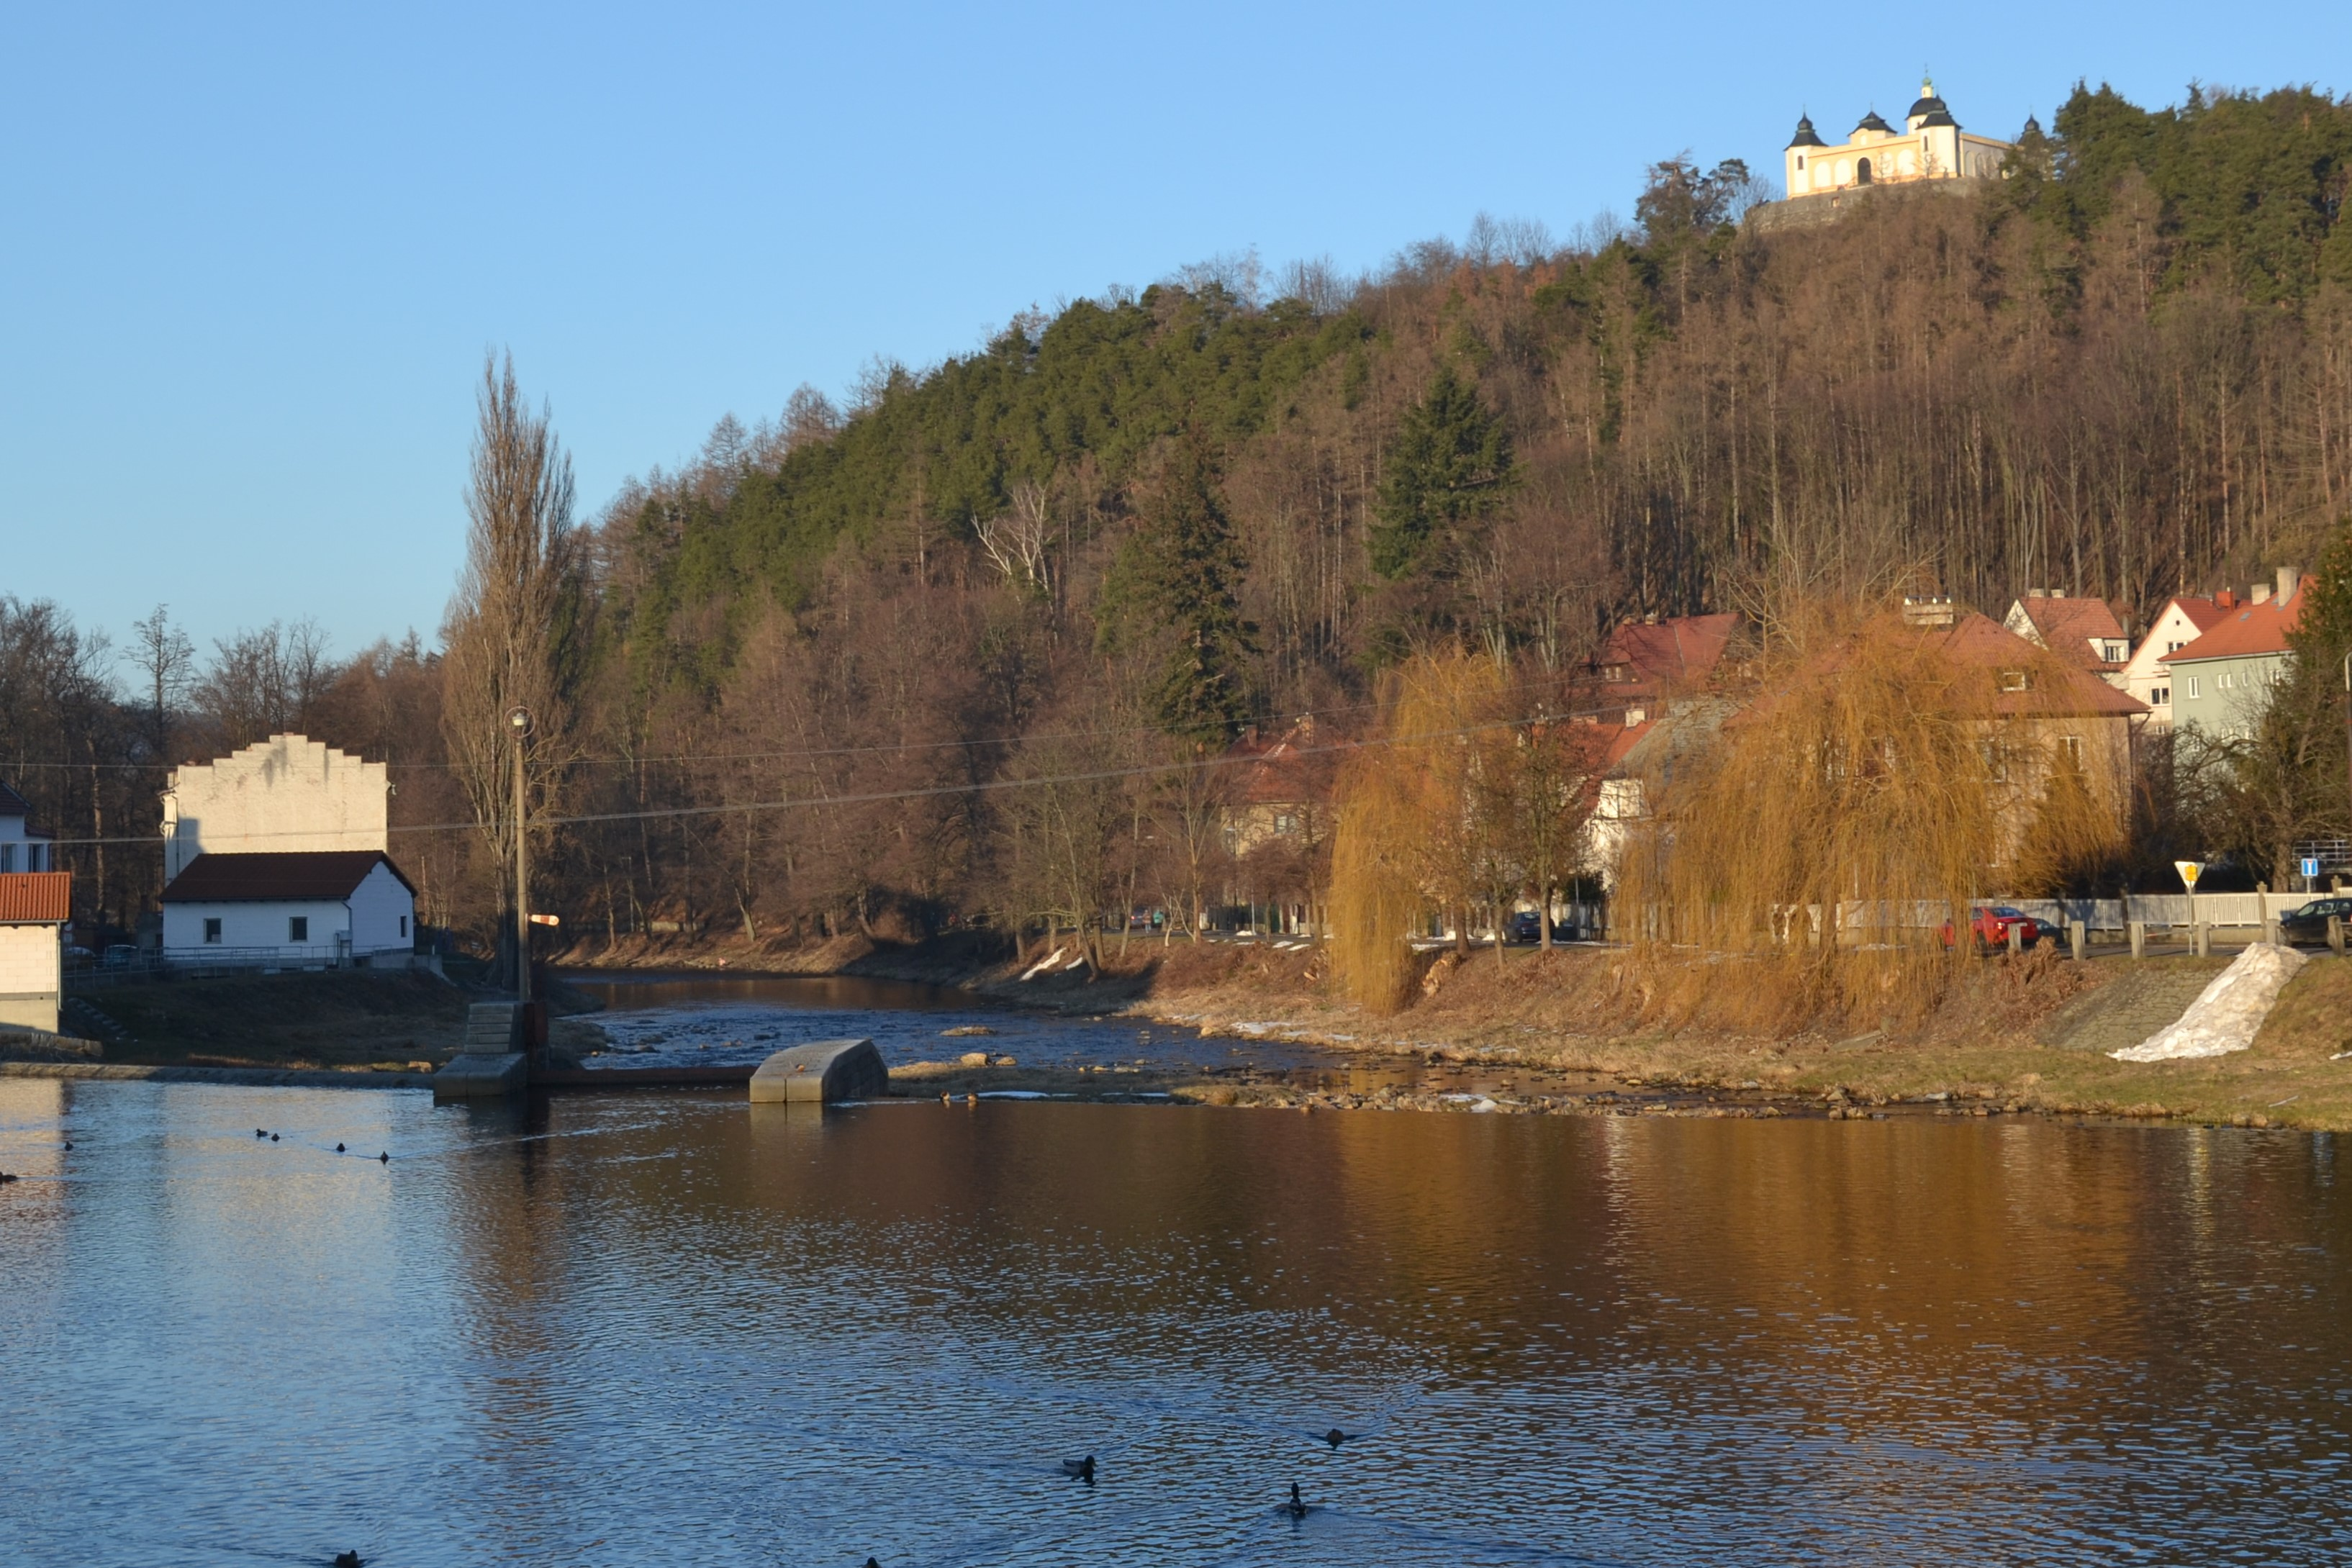
\includegraphics[width=12cm]{pics/susice.jpg}
	\caption{Otava v Sušici s kaplí svatých Andělů Strážných v pozadí}
	\label{obrazek:susice}
\end{figure}

Během 16. století začala Sušice ztrácet na své významnosti. Zásoby zlata byly téměř vyčerpány a během 50 let došlo k šesti velkým požárům města. Za~vlády Ferdinanda I. navíc přišla Sušice z důvodu odepření pomoci o všechna svá privilegia a statky, navíc byla nucena odvádět dávky z piva a vína. Přesto měla Sušice velké příjmy z obchodu, neboť městem procházela Zlatá stezka, dříve nazývaná také jako "pasovská" či "solná". Vzhledem k této výhodné pozici si město vydobylo právo svobodného skladování soli. Během třicetileté války bylo město poničeno táhnoucími se vojsky a z důvodu rekatolizace se mnoho obyvatel rozhodlo odstěhovat. 

Po třicetileté válce byla vybudována poutní kaple svatých Andělů Strážných. Ve 2. polovině 17. století postihla Sušici morová epidemie, kvůli které byl vybudován nový hřbitov a kaple svatého Rocha. Během národního obrození vzniklo v Sušici ochotnické divadlo a rozvíjela se výuka českého jazyka. V roce 1839 byla založena společnost SOLO na výrobu zápalek. V roce 1933 byl zřízen podnik PAP vyrábějící obaly. 

V dnešní době se v Sušici nachází mnoho turisticky vyhledávaných míst. Na~vrcholu hory Svatobor se nachází kamenná vyhlídková věž,  v Muzeu Šumavy Sušice lze nalézt jeden z největších mechanických betlémů v České republice a od roku 2014 byl v Sušici obnoven pivovar, který vaří pivo Sušičák. \cite{SMOOS} \cite{susice}


\subsection{Žichovice}
Na soutoku Nezdického potoka a Otavy se nachází malebná obec Žichovice. První písemnou zmínku lze nalézt z roku 1045, kdy Břetislav I. věnoval Žichovice břevnovskému klášteru. Ve 2. polovině 16. století koupil Žichovice Jan Kavka Říčanský z Říčan a nechal zde vybudovat renesanční tvrz. Tvrz byla kolem roku 1603 přestavěna Janem Libštejnským z Kolovrat na renesanční zámek. Od roku 1964 je zámek chráněn jako kulturní památka. \cite{zichovice}

Žichovice se nachází zhruba 1 km jižně od zříceniny Rabí (obrázek č. \ref{obrazek:zichovice}, zdroj \cite{rabi_foto}) . Hrad byl založen rodem Wittelsbachů již v první polovině 13.~století. S hradem se pojí mnoho pověstí, z nichž nejznámější je zřejmě pověst týkající se Jana Žižky, který zde údajně přišel o své druhé oko. Dohadů o~ztrátě oka je však mnoho. Mezi~nejrozšířenější pověsti patří pověst o veliteli hradu Přibíku Kocovském, který z hradeb Rabí vystřelil šíp, kterým zasáhl právě oko Jana Žižky. Tento výjev byl poté zobrazen i na rabské bráně. Podle jiné pověsti se zabodl šíp do~hrušně, pod níž Žižka stál, a tříska ze stromu mu vypíchla oko. Po mnoho let se poté v oblasti Rabí chovala tradice vysazování hrušní. \cite{rabi}

Pro obec Žichovice měla Otava velký historický význam. V okolí se nachází stará rýžoviště zlata. Je zde dlouhá vápenkářská tradice a bohatá historie voroplavby.

\begin{figure}[h!]
	\centering
	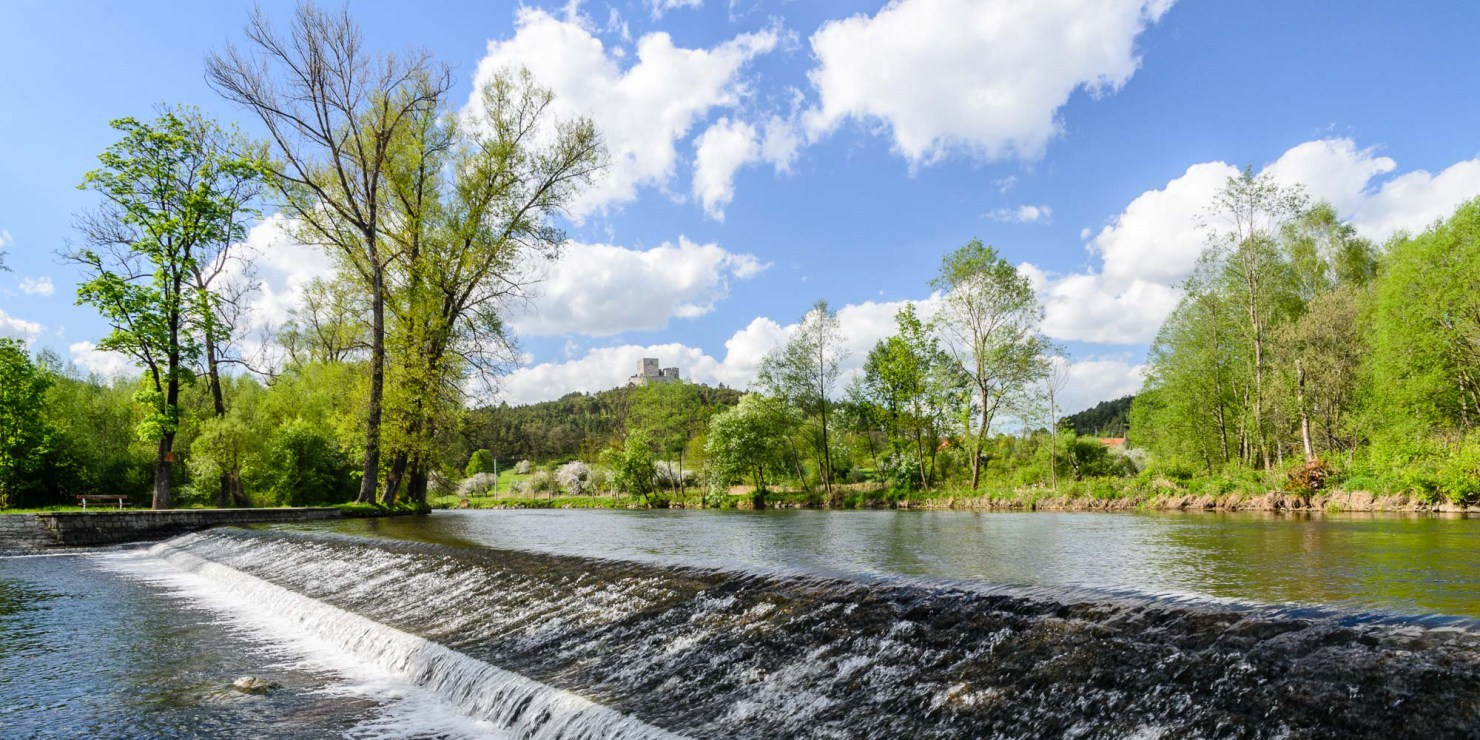
\includegraphics[width=12cm]{pics/zichovice.jpg}
	\caption{Žichovický jez, v pozadí zřícenina Rabí}
	\label{obrazek:zichovice}
\end{figure}

\subsection{Horažďovice}
Horažďovice leží v Horažďovické pahorkatině pod vrchem Prácheň. V roce 1293 byly Václavem II. povýšeny na město. Horažďovice, stejně jako Sušice a~Žichovice, byly využívány pro rýžování zlata a jako významný bod na obchodní stezce. O rozvoj města se nejvíce zasloužil rod Bavorů ze Strakonic. 

V Horažďovicích lze nalézt mnoho významných budov. Za zmínku stojí rozhodně zámecký komplex s panským pivovarem nacházející se na náměstí. V tomto zámku se nachází velký sál s freskovou výzdobou  (obrázek č. \ref{obrazek:hd}, zdroj \cite{hd}). Nástropní freska zachycuje bitvu husitů a císaře Zikmunda pod~Vyšehradem. Stěny sálu jsou pokryty výjevy z válek s Turky za vlády Leopolda I.  \cite{obce}\cite{hd}

\begin{figure}[h!]
	\centering
	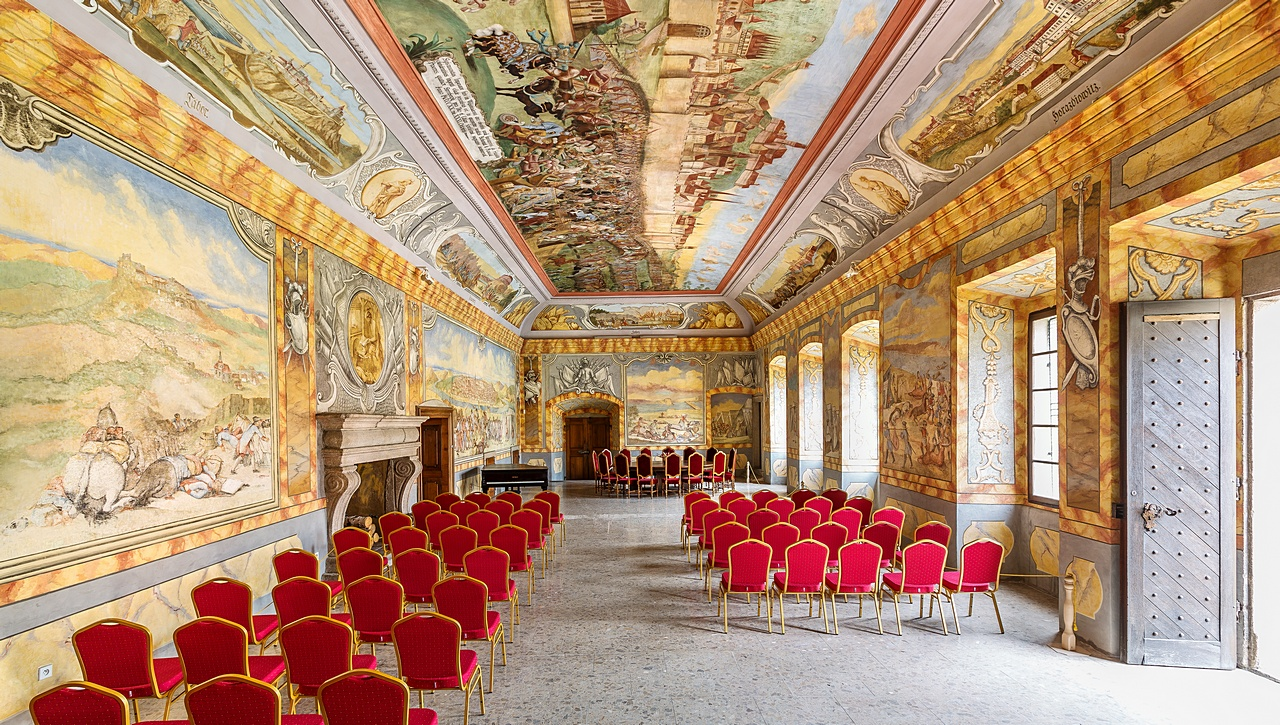
\includegraphics[width=11cm]{pics/hd.jpg}
	\caption{Velký sál v Horažďovicích}
	\label{obrazek:hd}
\end{figure}



\subsection{Strakonice}
Strakonice, okresní město ležící v jižních Čechách na soutoku Otavy a Volyňky. Vzniklo spojením čtyř osad - Strakonic, Bezděkova, Lomu a Žabokrt. O~Strakonicích pochází první písemná zmínka z roku 1243, kdy Bavor I. se~svou manželkou Bolemilou věnuje okolní vsi, kostel a část hradu řádu johanitů. Ve~2. polovině 13. století nechává Bavor II. postavit hradní věž Rumpál, která stojí dodnes. 

\begin{figure}[h!]
	\centering
	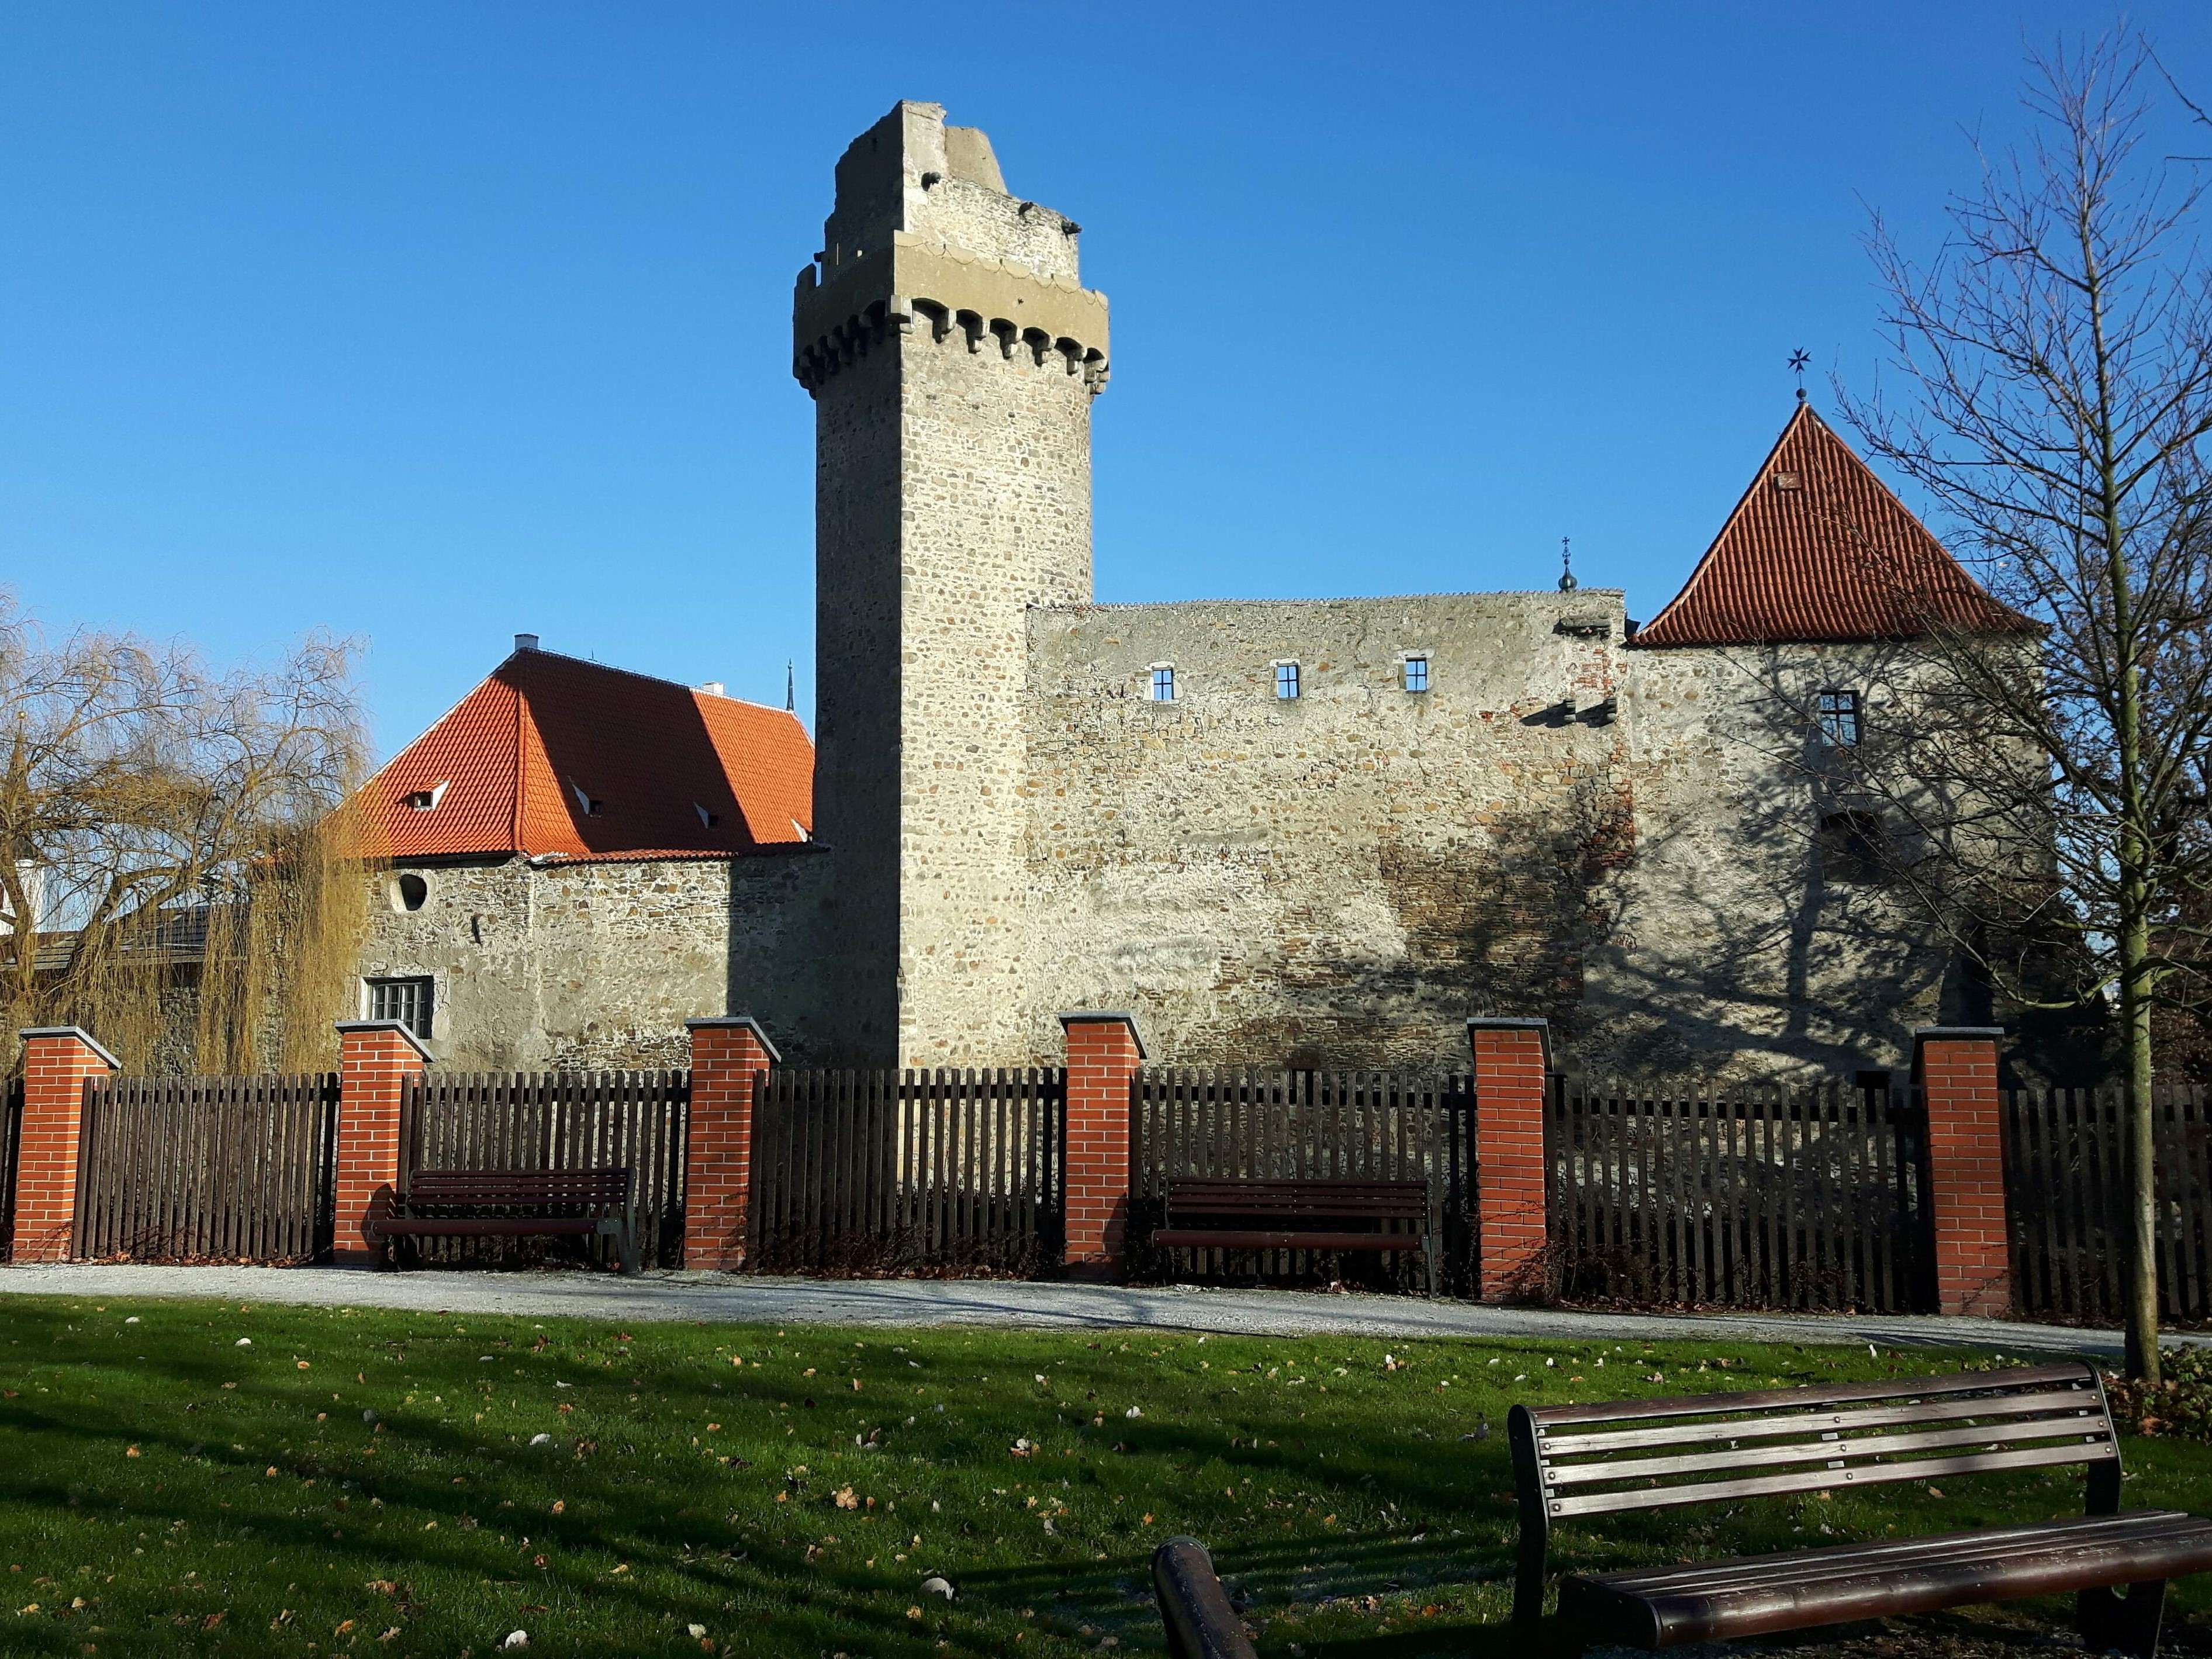
\includegraphics[width=11cm]{pics/hrad.jpg}
	\caption{Pohled na Strakonický hrad ze západní strany}
	\label{obrazek:hrad}
\end{figure}

V roce 1367 bylo městu Bavorem IV. uděleno právo várečné. Pivo si vařili měšťané ve vlastních domech\footnote{Uvádí se, že v polovině 17. století se ve Strakonicích nacházelo až 158 domů s právem vařit pivo} a vrchnost v hradním pivovaru. V roce 1649 došlo k uskupení právovárečníků a byl založen měšťanský pivovar. Ten stojí ve~Strakonicích dodnes a je to poslední pivovar v České republice, který je ve~vlastnictví města. 

V roce 1357 postihl město velký požár, který zničil horní část města. Při~obnově bylo náměstí v této části rozšířeno, díky čemuž se protáhlo a mělo tvar dlouhého úzkého obdélníku. Obyvatele Strakonic dodnes tíží fakt, že místo náměstí mají spíše dlouhou ulici. Kromě požárů sužovaly město zejména povodně. Ty byly velmi časté a opakovaně zaplavovaly podhradí. Z toho důvodu neviděli Bavorové oblast Strakonicka za vhodnou pro založení města.

Během husitských válek byly Strakonice na straně katolického panstva a~šlechtických rodů. Pro husitská vojska byl hrad nedobytný. Dobylo jej až~během třicetileté války v roce 1619 císařské vojsko pod vedením Karla Longuevala. Město bylo drancováním švédskými vojsky natolik zdevastováno, že~jej v roce 1645 velkopřevor Rudolf Colloredo z Wallsee osvobodil od placení válečných daní.

Po první světové válce byl hrad prodán agrárnímu sdružení a ve~městě se začal rozvíjet průmysl. Vznikla Jihočeská zbrojovka a ve velkém se ve~Strakonicích vyráběly turecké čepičky (fezy), které byly následně nahrazeny barety. 

Ze Strakonic pochází mnoho významných osobností, za zmínku určitě stojí František Ladislav Čelakovský nebo Josef Šmidinger. Do Strakonic také zasadil svou báchorku o Strakonickém dudáku Josef Kajetán Tyl. Ve Strakonicích prožil své dětství Jiří Žáček a Josef Skupa a jednou z nejdůležitějších osobností byl Josef Režný, který založil Prácheňský soubor lidových písní a tanců (Prácheňáček) a byl spoluzakladatelem Jihočeské slavnosti písní a tanců. Dnes známý jako Mezinárodní dudácký festival ve Strakonicích. \cite{obce}


\subsection{Písek}
Vznik Písku se datuje zhruba do poloviny 13. století. Město vzniklo v oblasti rýžoviště zlatého písku, z čehož lze usuzovat i původ jména města. V roce 1254 jej rozšířil Přemysl Otakar II. na královské město. Během 13. století vzniklo v Písku mnoho významných staveb: hrad, klášter, děkanský kostel, rychta a~kamenný most (obrázek č. \ref{obrazek:pisek}, zdroj: \cite{pisek}), který je v současné době nejstarším kamenným mostem v~České republice. 

\begin{figure}[h!]
	\centering
	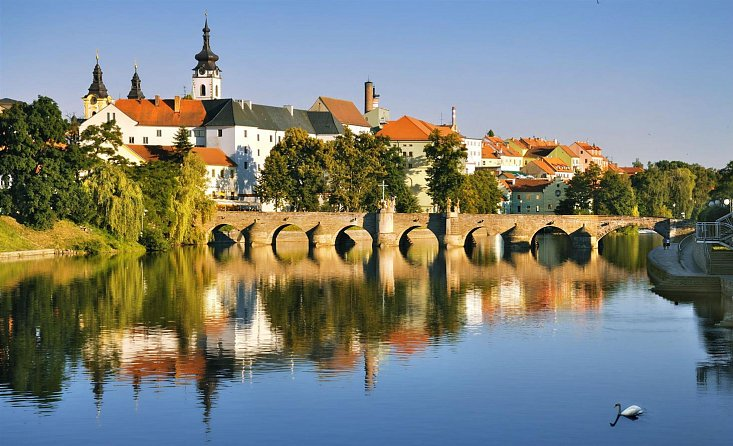
\includegraphics[width=11cm]{pics/pisek.jpg}
	\caption{Kamenný most v Písku}
	\label{obrazek:pisek}
\end{figure}

Písek byl ve 13. století jmenován na sídlo Prácheňského kraje. Během husitských válek bylo město centrem Jednoty táborské a Jan Žižka z Trocnova jej často navštěvoval. Za třicetileté války bylo město dobyto a vydrancováno. V 18. století se mu však opět vrátila všechna sláva a bohatství a v roce 1778 bylo v Písku otevřeno gymnázium. Písek bylo třetí české město, ve kterém bylo zřízeno elektrické osvětlení obloukovými lampami Františka Křižíka. Jedním z~nejznámějších obyvatel města je však Fráňa Šrámek, který Písek často používal jako dějiště svých děl. 

V současnosti je město jedním z vyhledávaných turistických cílů. Kromě zmíněného nejstaršího kamenného mostu se v Písku nachází několik kostelů a~kaplí, sladovna a Prácheňské muzeum. \cite{pisek} \cite{pisek2}

\section{Významné skutečnosti související s Otavou}
\subsection{Rýžování zlata}
Hojné osídlení podél řeky Otavy bylo v minulosti dáno zejména četnými nálezy zlata v řece. Zlato se získávalo tzv. rýžováním. Při rýžování se do kovové pánve nabere směs písku z řeky a následnými krouživými pohyby na hladině jsou postupně lehké částice odplavovány a zlato zůstává na dně pánve. \cite{zlato}

Na Otavě se zlato rýžuje dodnes. V Kestřanech se koná každoročně soutěž v rýžování zlata, která probíhá v režii Českého klubu zlatokopů. 

\subsection{Voroplavba}
První zmínky o plavení dřeva na Otavě pochází již ze 14. století za doby vlády Jana Lucemburského. Šumavské dřevo bylo tehdy považováno za jeden z nejkvalitnějších stavebních materiálů a za vlády Karla IV. se nesmělo stavět z~jiných, než ze šumavských. Vysoká kvalita byla dána zejména tím, že vymáčené dřevo již dále nepracovalo a při vysoušení se nekroutilo a nepraskalo. 

V 19. století začala vznikat vaziště, ve kterých byly jednotlivé kusy dřeva vázány dohromady. Vaziště vzniklo např. v Dlouhé Vsi, v Žichovicích nebo v Katovicích. Vorařům se často přezdívalo "Hamburáci", neboť dřevo často plavili až do Hamburku. 

Po 2. světové válce začala významnost voroplavby upadat a při transportu se dávala přednost železniční a automobilové dopravě. V roce 1954 byla dokončena stavba vodní nádrže Slapy, která plavení dřeva definitivně ukončila. Paradoxně bylo dřevo pro tuto stavbu dopravováno po řece. Poslední vor na~Otavě vyplul 12. září 1960. Historické fotografie a dokumenty zachycující voroplavbu jsou dodnes k vidění v Muzeu řeky Otavy a voroplavby ve Střelských Hošticích. 

Na obrázku č. \ref{obrazek:voroplavba} lze vidět dochovanou historickou fotografii poblíž Strakonického pivovaru. Fotografie pochází ze soukromé sbírky Ladilslava Hölla a~byla pořízena v roce 1920.

\clearpage
\begin{figure}[h!]
	\centering
	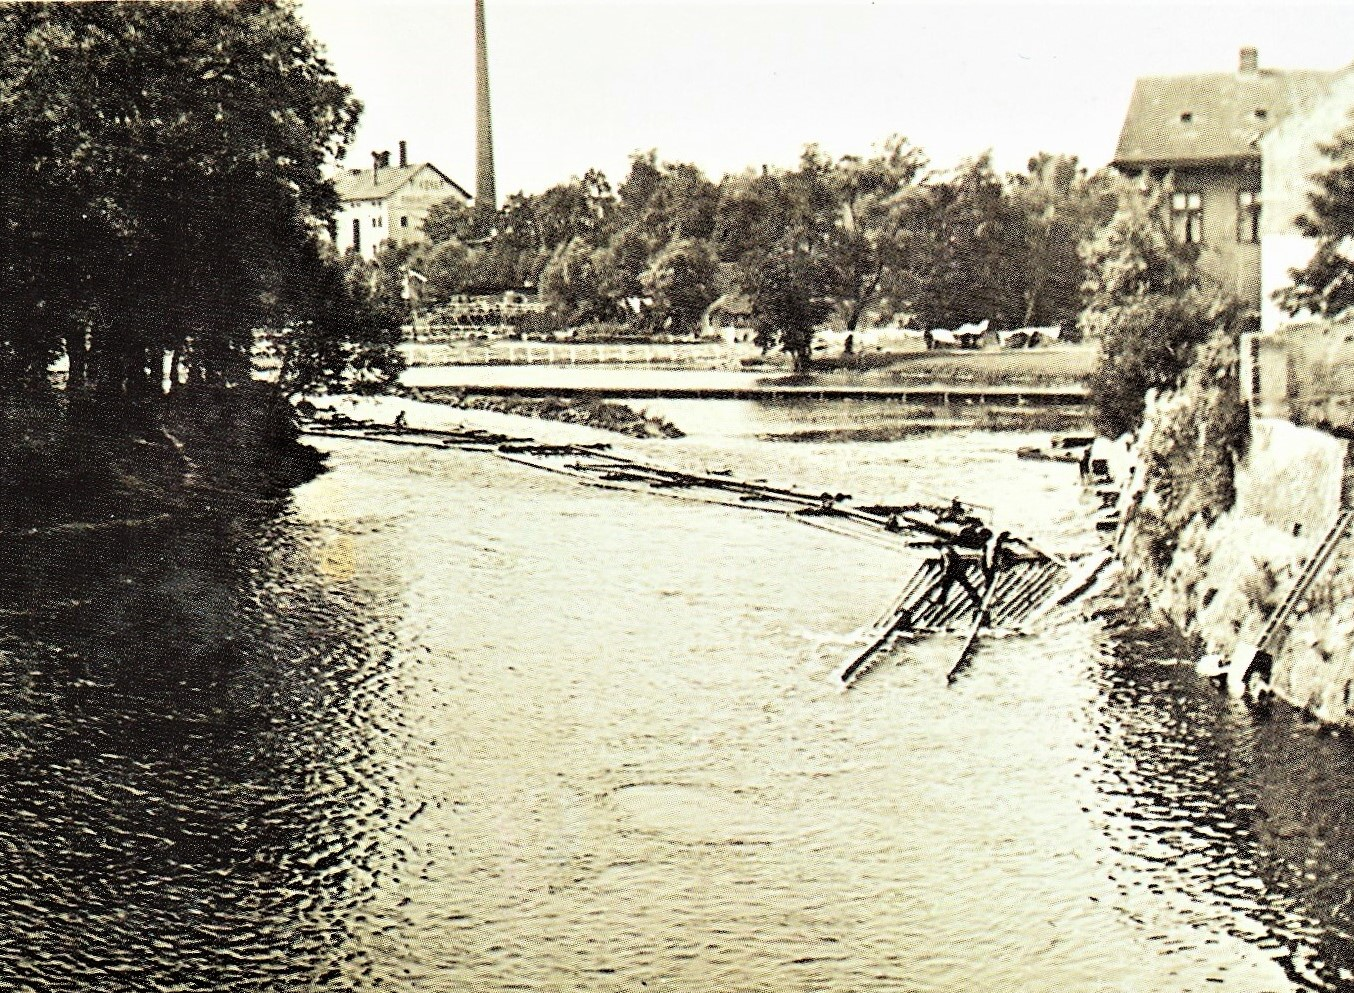
\includegraphics[width=11cm]{pics/voroplavba.jpg}
	\caption{Voroplavba ve Strakonicích, 1920}
	\label{obrazek:voroplavba}
\end{figure}


\subsection{Povodeň v roce 2002}
V roce 2002 postihla Českou republiku silná povodeň. Byla to jedna z největších katastrof současnosti a mezi nejvíce postižené oblasti patřily jižní Čechy. Velké množství vody zatopilo téměř všechna města po proudu. V Písku povodeň dokonce poničila kamenný most. 

\begin{figure}[htp]
\centering
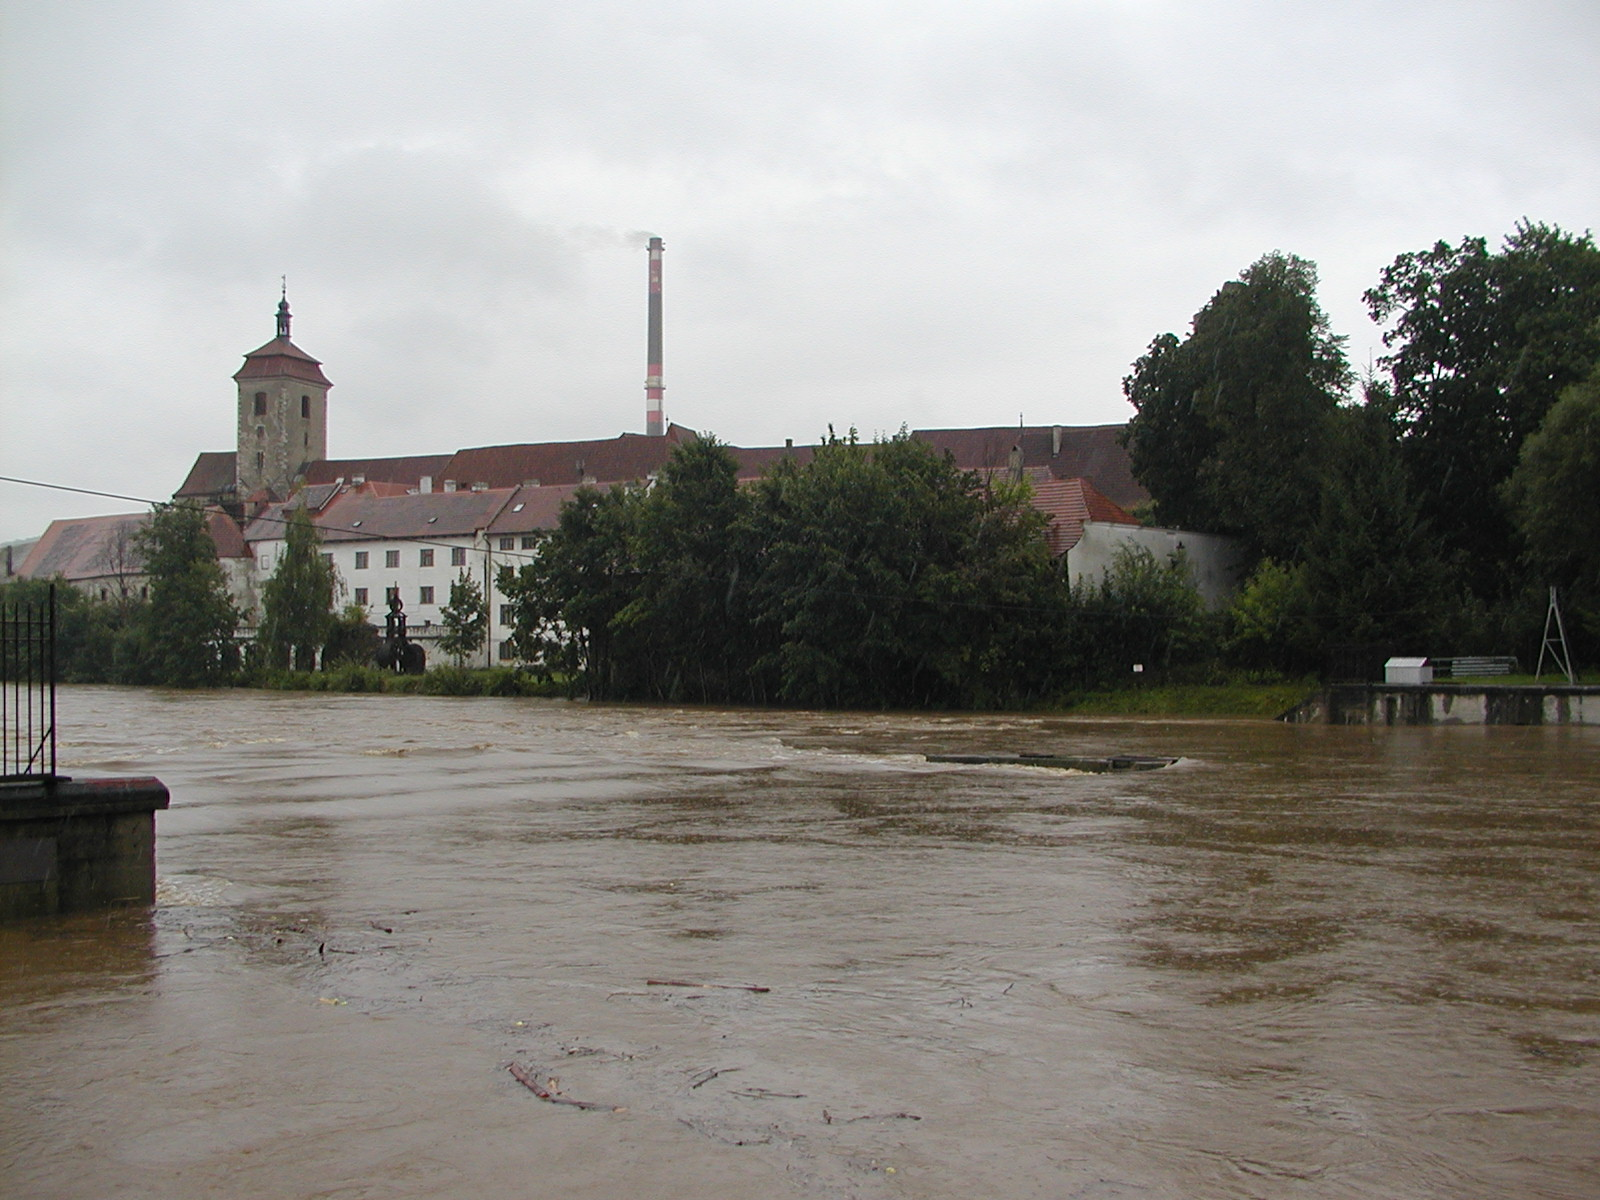
\includegraphics[width=6cm]{pics/povoden1.jpg}
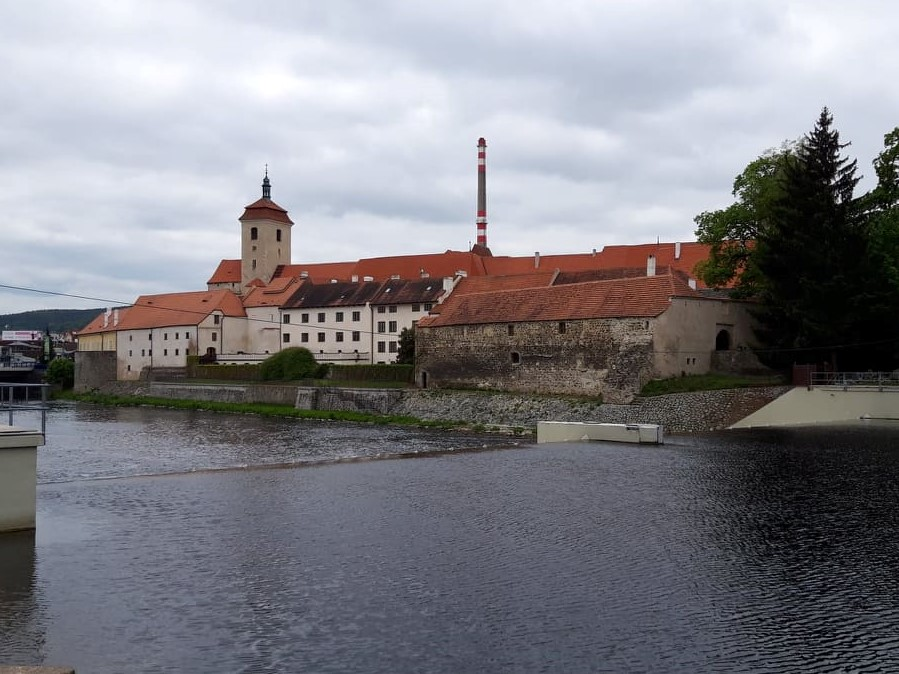
\includegraphics[width=6cm]{pics/povoden1_2019.jpg}
\caption{Povodeň v roce 2002 a aktuální stav – Strakonický hrad}
\label{obr:povoden_hrad}
\end{figure}

\begin{figure}[h!]
\centering
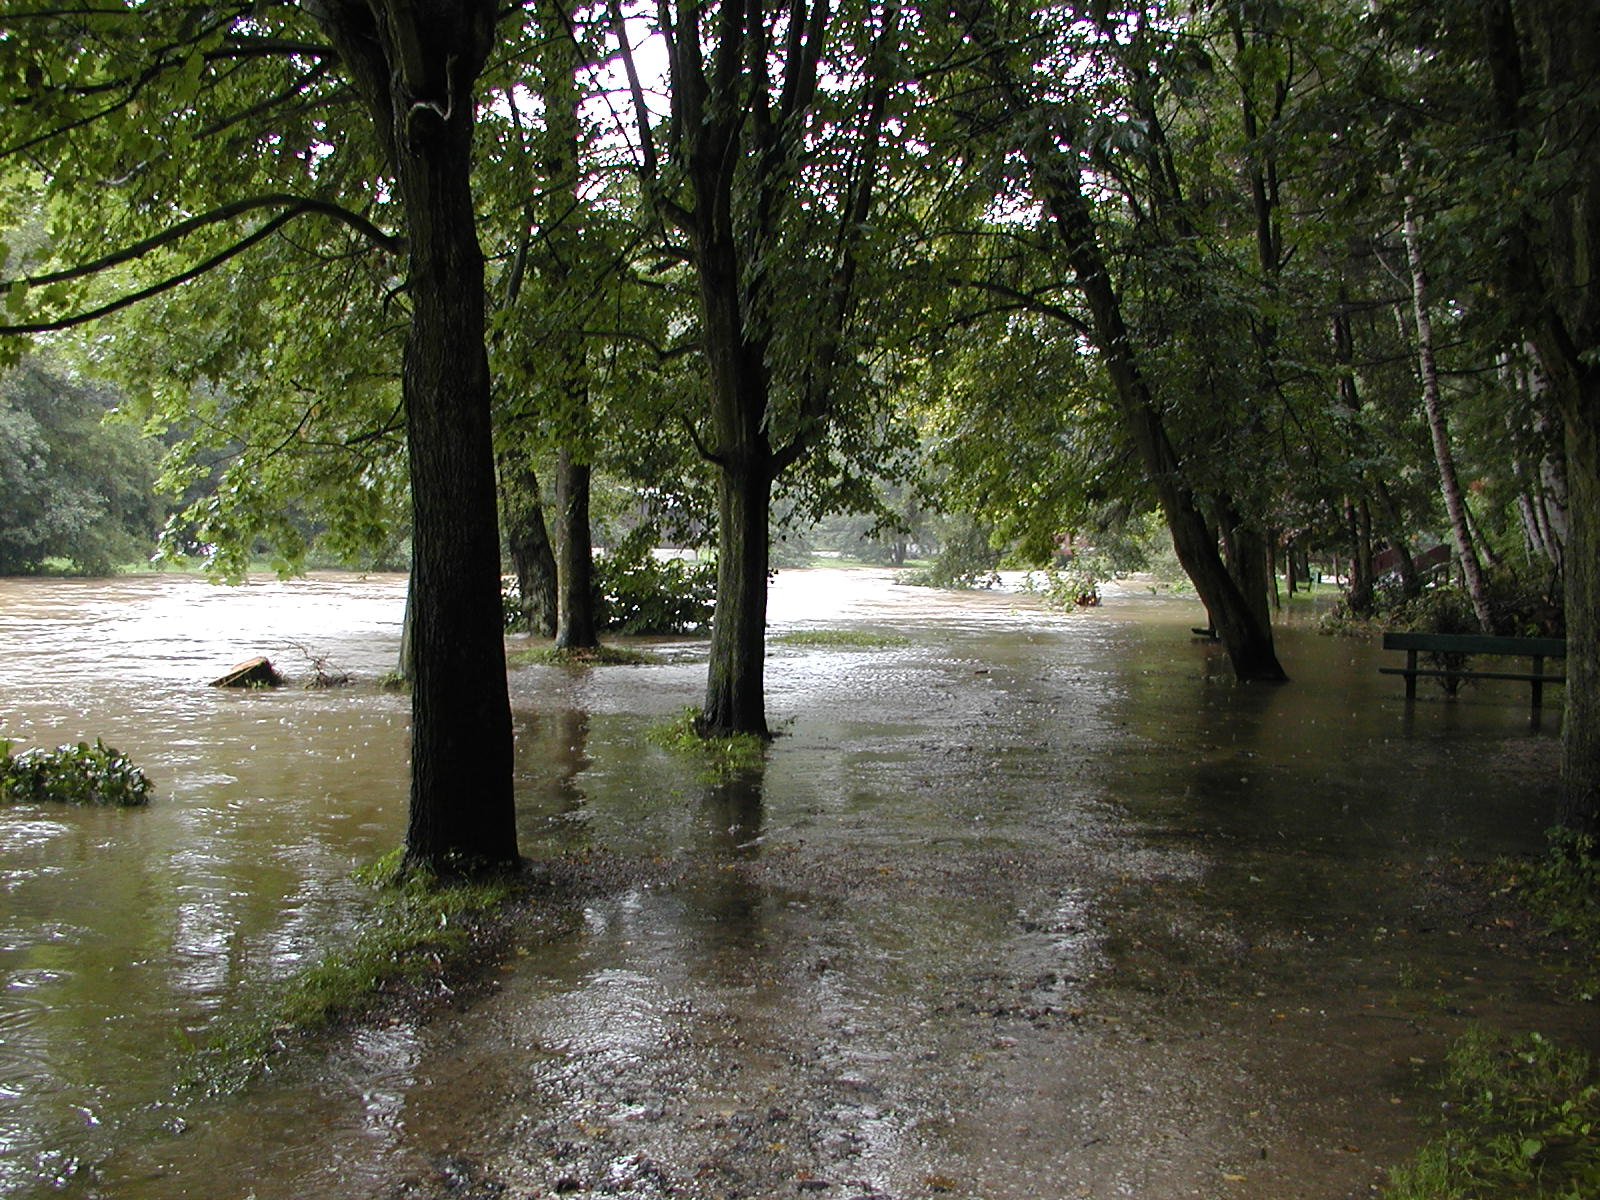
\includegraphics[width=6cm]{pics/povoden2.jpg}
\includegraphics[width=6cm]{pics/povoden2_2019.jpg}
\caption{Povodeň v roce 2002 a aktuální stav – Podskalí}
\label{obr:povoden_hrad}
\end{figure}

\begin{figure}[h!]
\centering
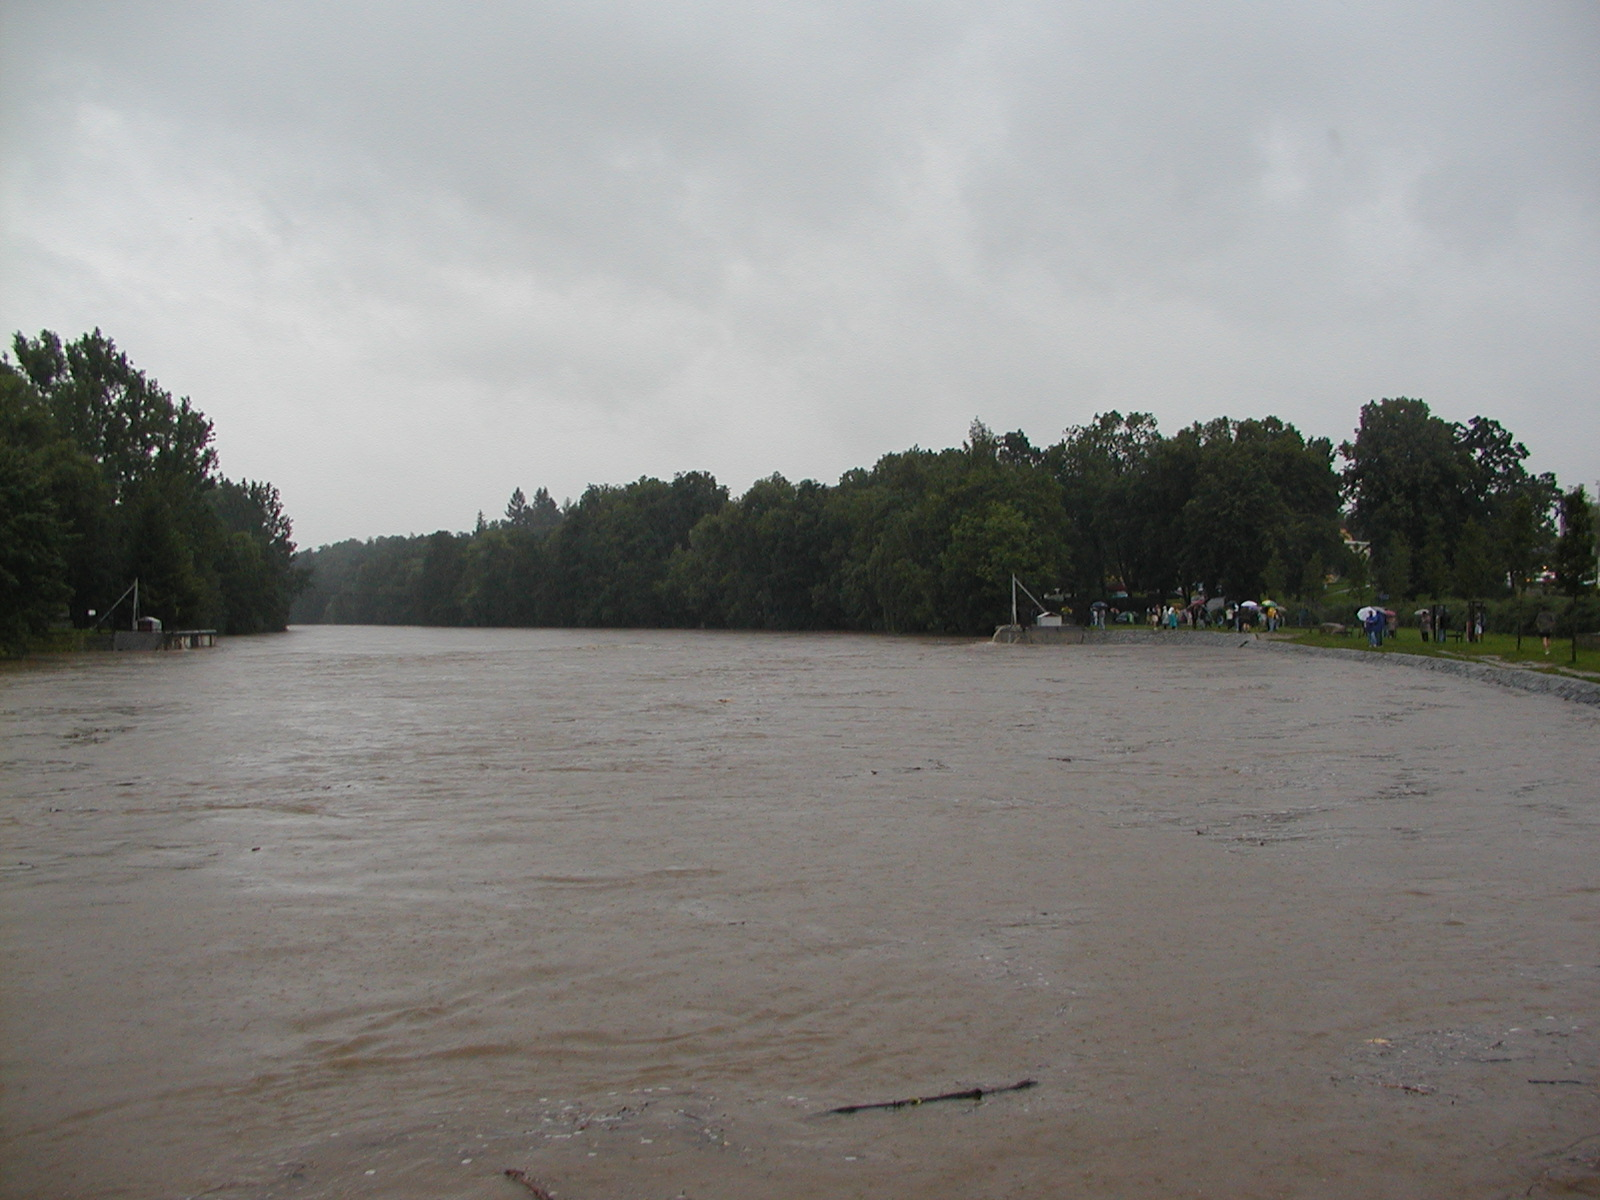
\includegraphics[width=6cm]{pics/povoden3.jpg}
\includegraphics[width=6cm]{pics/povoden3_2019.jpg}
\caption{Povodeň v roce 2002 a aktuální stav – Pětikolský jez}
\label{obr:povoden_hrad}
\end{figure}

\begin{figure}[h!]
\centering
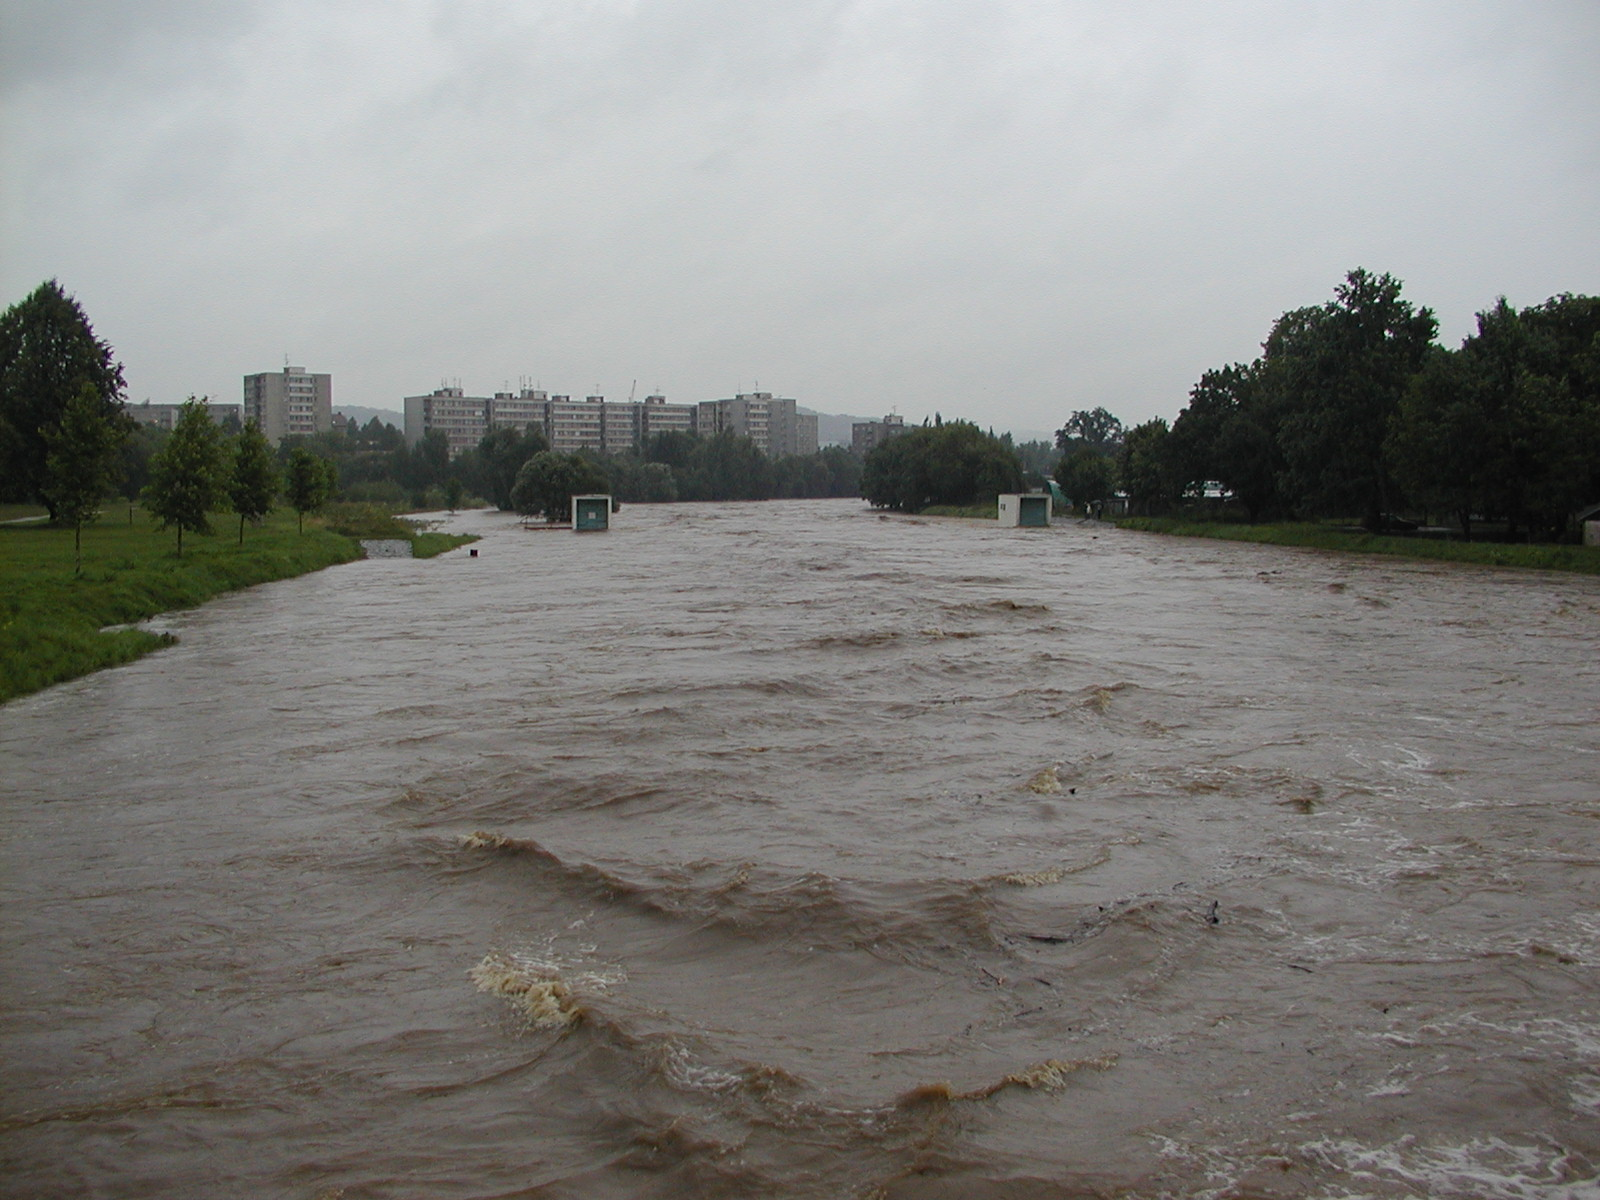
\includegraphics[width=6cm]{pics/povoden4.jpg}
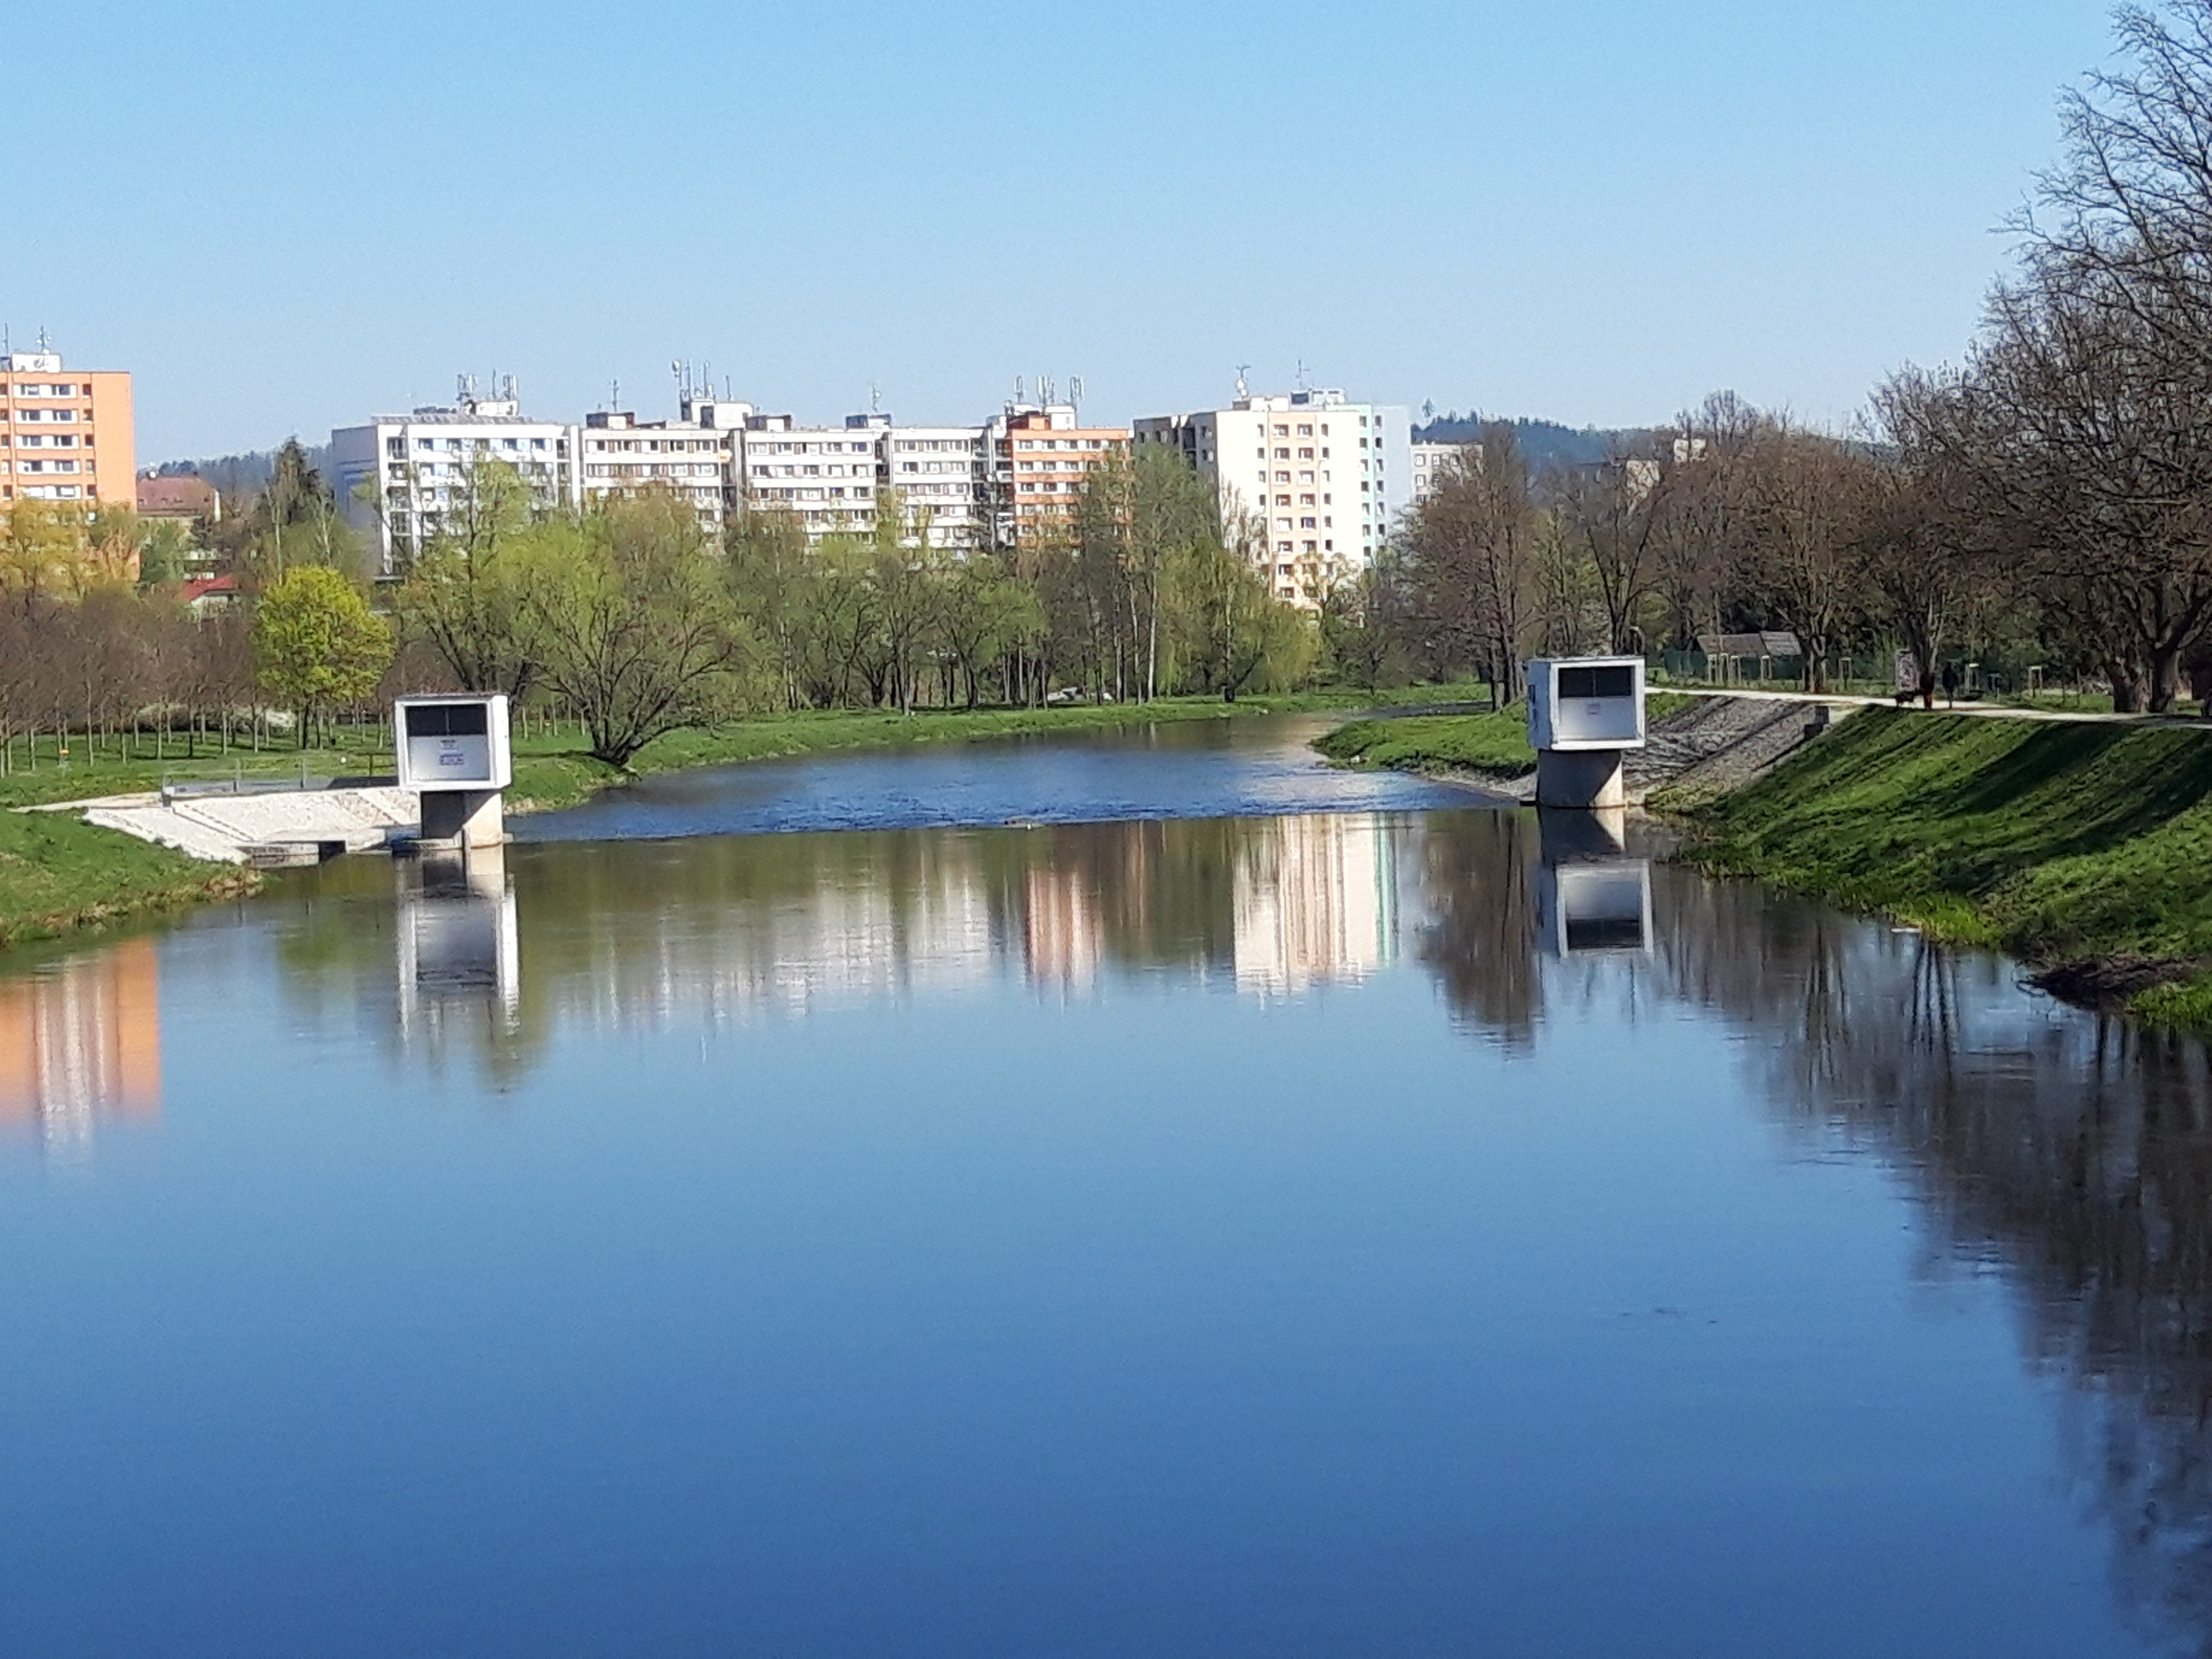
\includegraphics[width=6cm]{pics/povoden4_2019.jpg}
\caption{Povodeň v roce 2002 a aktuální stav – Křemelka}
\label{obr:povoden_hrad}
\end{figure}

\chapter{Použitá data}
\section{Stavební plány Strakonického hradu}
Pro tvorbu 3D modelu Strakonického hradu byly použity stavební plány, které poskytl Stavební úřad ve Strakonicích. 

Stavební úřad měl k dispozici vypracované podklady získané stavebně historickým průzkumem (SHP). SHP je metoda, která kompletně vypracuje a~zhodnotí historicky významnou stavební památku či historické jádro některých českých a moravských měst. Mezi prvními, kdo SHP prováděl, byl Kamil Hilbert na počátku 20. století. Následoval ho Oldřich Stefan z Ústavu dějin architektury ČVUT a doc. Václav Mencl z Filozofické fakulty Univerzity Karlovy. Po 2. světové válce bylo zdevastováno mnoho měst a významných památek. Z tohoto důvodu vznikl ústav R-ateliér, který rekonstruoval památky při organizaci Stavoprojekt. V roce 1954 byl R-ateliér přejmenován na Státní ústav pro rekonstrukce památkových měst a objektů (SÚRPMO). V~\mbox{SÚRPMO}~působilo několik významných osobností. Za zmínku jistě stojí Dobroslav Líbal nebo Jan Muk. 

Mezi materiály, které měl k dispozici Stavební úřad ve Strakonicích, patří i vypracované podklady z SHP. Tyto materiály pochází ze 70. let 20. století, jsou v perfektním stavu a velmi detailně vypracovány. Na každém listu je ručně zakreslený erb Strakonic. Autor odvedl precizní a velmi kvalitní práci. Tyto materiály mají však v dnešní době vysokou hodnotu, tudíž nebylo možné je za účelem tvorby 3D modelu zapůjčit. Z tohoto důvodu byly použity plány vzniklé na počátku 21. století. \cite{shp}

\clearpage

\begin{figure}[h!]
	\centering
	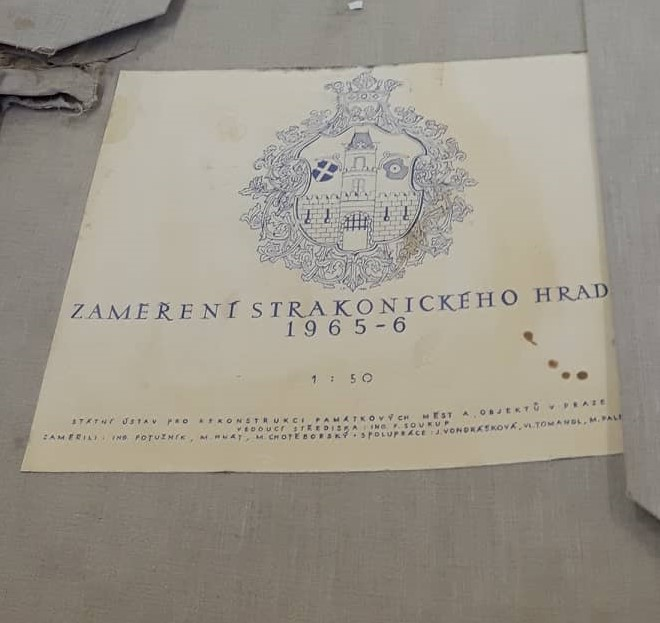
\includegraphics[width=10cm]{pics/shp.jpg}
	\caption{Úvodní list materiálů ze stavebně historického průzkumu Strakonického hradu}
	\label{obrazek:shp}
\end{figure}


\section{Kartografické podklady}
\subsection{Císařské povinné otisky map stabilního katastru}
Císařské povinné otisky map stabilního katastru vznikaly na základě císařského patentu Františka I. z roku 1817. Aby byly mapy po celém území vyhotoveny stejným způsobem, byla v roce 1824 vydána měřická instrukce. Mapy vznikly za účelem přesného mapového podkladu pro stanovení pozemkové daně. Základní délkovou jednotkou byl vídeňský sáh [$^\circ$] (1\,$^\circ$~=~1,896484\footnote{Odvozeno od výšky dospělého muže}~m).

Kartografické zobrazení těchto map bylo Cassini-Soldnerovo (transverzální válcové zobrazení). Kladná osa Y směřovala k západu a kladná osa X k~jihu. Jednalo se o zobrazení ekvidistantní v kartografických polednících, což znamená, že se vzdáleností od základního poledníku roste i velikost délkového zkreslení. Z tohoto důvodu bylo potřeba vytvořit několik soustav. Pro Rakousko–Uhersko jich bylo použito 7. Při volbě soustav se vycházelo z požadavku na maximální zkreslení 50 cm/km. 

Na našem území byly použity tři soustavy. Jednalo se o soustavy s počátečním bodem Gusterberg (Horní Rakousy), sv. Štěpán (Vídeň) a Gellérthégy (Budapešť). V roce 1887 byla vydána nová měřická dokumentace, která již používala metrickou soustavu. Císařské povinné otisky byly původně uloženy v~Centrálním archivu pozemkového katastru ve Vídni. V rámci tzv. archivní rozluky byly po rozpadu Rakousko-Uherska převezeny do Prahy. Legendu těchto map můžete vidět na obrázku č. \ref{obrazek:legenda} (zdroj: \cite{cpo_legenda}). \cite{mapko}


\begin{figure}[h]
	\centering
	\includegraphics[width=13cm]{pics/legenda_CPO.png}
	\caption{Legenda císařských povinných otisků stabilního katastru}
	\label{obrazek:legenda}
\end{figure}

\subsection{Katastrální mapa}
Katastrální mapa je státní mapové dílo vydávané Českým úřadem zeměměřickým a katastrálním. Jedná se o mapy velkého měřítka (1 : 1000, 1 : 2880 apod.). Katastrální mapy jsou zpravidla vedeny v S–JTSK. Jejich hlavní využití je při zjišťování umístění pozemku v území a jako podklad pro územní a~stavební řízení, pro řízení o vyvlastnění pozemku apod. 

3 hlavní složky katastrální map jsou polohopis, popis a body. Polohopis obsahuje například hranice katastrálních území, státní hranice či hranice nemovitostí. Popis zahrnuje měřítko, označení sousedních mapových listů, označení parcel parcelními čísly nebo pomístní názvosloví\footnote{U digitálních map jsou mimorámové údaje obsaženy v metadatech}. Body jsou obsaženy pouze v~mapách, které jsou v S–JTSK a jedná se o body polohových bodových polí. \cite{cuzk}

\subsection{Státní mapa odvozená v měřítku 1 : 5 000}
Státní mapa odvozená, známá pod zkratkou SMO–5, je nejrozšířenějším státním mapovým dílem v měřítku 1 : 5 000. SMO–5 obsahuje polohopis, výškopis, popis a mimorámové údaje. Mapa je v souřadnicovém systému S–JTSK, výšky jsou v systém Bpv. Každý list zobrazuje plochu o velikosti 2,5~$\times$~2,0~$km^{2}$. Území České republiky je pokryto 16 193 listy. 

Polohopis u SMO–5 byl tvořen fotomechanickou transformací polohopisu katastrální mapy. U map byla zavedena průměrná srážka mapových listů katastrálních map 0,7 \%, která měla zajistit plynulý přechod mezi jednotlivými listy. Polohopis bylo nutné generalizovat. Při generalizaci byly vypuštěny stavební parcely s šířkou menší než 1 mm v měřítku 1 : 2 880 a parcely s plochou menší než 1 $mm^{2}$ v měřítku 1 : 5 000. Úzké parcely, které byly v měřítku 1 : 5 000 užší než 1 mm byly zobrazeny jednou čarou. V mapách byla zcela vypuštěna parcelní čísla. Výškopisná složka byla přebírána z příložných a topografických map fotomechanickou transformací. \cite{cuzk} \cite{smo5_bp}




\subsection{Ortofoto}
Ortofoto je v dnešní době jeden z nejznámějších a nejpoužívanějších kartografických produktů vzniklých leteckou fotogrammetrií. Ortofoto vzniká mozaikou letecky měřených snímků. Opravením těchto snímků o výškové poměry daného území je výsledný produkt prezentován jako kolmý průmět terénu do~roviny. Snímkování České republiky je prováděno každé dva roky, přičemž každý rok je zpracována polovina území. V roce 2019 je snímkována západní část Česka.

Tvorba státního Ortofota ČR je zajištěna od roku 2003 Zeměměřickým úřadem ve spolupráci s Vojenským geografickým a hydrometeorologickým úřadem na základě dohody ČÚZK s Ministerstvem obrany ČR. Ortofota jsou v~dnešní době hojně vyhledávaná i ze stran laické veřejnosti. Jejich obliba je zapříčiněna zejména přehledností a zobrazením skutečných barev, díky čemuž jsou mapy pro mnoho uživatelů i lépe čitelné. \cite{cuzk} \cite{ortofoto}


\subsection{Digitální model reliéfu 5. generace}
Digitální model reliéfu České republiky 5. generace digitálně znázorňuje zemský povrch Česka body o třech souřadnicích (X, Y, H), kde H představuje výšku v systému Bpv. Tento model vznikl metodou leteckého laserového skenování v letech 2009 – 2013. V zalesněném území dosahuje střední souřadnicové chyby 0,3 m, v odkrytém území je střední souřadnicová chyba kolem 0,18 m. Model neobsahuje budovy a je určen především k analýzám terénních poměrů. \cite{cuzk}



\section{Fotodokumentace}
Součástí této práce je také vyhledání historických fotografií a jejich případné porovnání se současným stavem. Z historických fotografií byly použity fotografie ze sbírky Ladislava Hölla a z webových stránek Fotohistorie \cite{fotohistorie} a Šumava \cite{sumava}. Dále byly prozkoumány archivní publikace, ze kterých byly použité fotografie vyfotografovány pro následné použití v této práci.

Kromě fotografií bylo využito i historických pohlednic zachycujících Otavu nebo Strakonický hrad. Zároveň byly použity i rytiny a kresby.




\chapter{Rovinné transformace}
V rámci práce byla potřebná důkladná znalost transformace, která byla využita při georeferencování mapových podkladů. Transformací lze označit proces, při němž dochází k přechodu z jedné soustavy do druhé. Pro každý druh transformace je požadované odlišné množství identických bodů, tedy takových bodů,  jejichž souřadnice jsou známy a jejichž poloha lze jednoznačně identifikovat v~obou soustavách.

Při výpočtu transformací je hlavním cílem výpočet transformačního klíče. Transformační klíč umožňuje převod souřadnic z jedné soustavy do druhé a obsahuje v sobě hodnotu posunu počátků souřadnicových systémů, stočení souřadnicových os a změnu měřítka. K jeho určení je potřebná znalost nutného či nadbytečného počtu identických bodů. 

V této kapitole se vycházelo zejména z díla Jiřího Cajthamla \textit{Analýza starých map v digitálním prostředí na příkladu Műllerových map Čech a Moravy}, ze studijního materiálu od Zdeňka Skořepy \textit{Geodézie 4}, z bakalářské práce Jany Malimánkové \textit{Tvorba datového modelu Crigingerovy mapy v ArcGIS} a~z~nápovědy k programu ArcGIS. V rámci aplikace ArcMap je možné při georeferencování zvolit transformaci podobnostní, polynomickou, křivkovou, vyrovnávací či projektivní. V této kapitole budou tyto typy transformací stručně popsány. \cite{transformace} \cite{skorepa} \cite{gis_transformace} \cite{vugtk} \cite{malimankova}

\

Transformace lze nejjednodušeji zapsat rovnicí \eqref{zaklad_tr}, kde neznámé \textit{x', y'} vyjadřují souřadnice v cílové soustavě a \textit{x, y} souřadnice v počáteční soustavě. Matici \textbf{\textit{P}} lze následně rozepsat do výrazu \eqref{zaklad_tr2}, v níž neznámá \textbf{\textit{T}} označuje posunutí (translaci), \textbf{\textit{R}} značí rotaci a \textbf{\textit{M}} měřítko.

\begin{align}\label{zaklad_tr}
\textbf{x}' = \textbf{P} \cdot \textbf{x}
\end{align}

\begin{align}\label{zaklad_tr2}
\textbf{x}' = \textbf{T} \cdot \textbf{R} \cdot \textbf{M} \cdot \textbf{x}
\end{align}

Posunutí vyjadřuje vzájemné posunutí počátku souřadnicových soustav a~lze maticově zapsat:

\begin{align} \label{matT}
\boldsymbol {T (X_t, Y_t)}= \begin{pmatrix}
    1 & 0 & X_t \\
    0 & 1 & Y_t \\
    0 & 0 & 1 
\end{pmatrix}
\end{align}

Rotace udává otočení bodu kolem středu vztažné soustavy o daný úhel proti směru hodinových ručiček. Obecně lze matici rotace zapsat:

\begin{align} \label{matR}
\boldsymbol {R (\omega_x, \omega_y) }= \begin{pmatrix}
    cos(\omega_x) & -sin(\omega_y) & 0 \\
    sin(\omega_x) & cos(\omega_y) & 0 \\
    0 & 0 & 1 
\end{pmatrix}
\end{align}

Měřítko udává poměr vzdálenosti dvou identických bodů. Pokud je absolutní hodnota měřítka v intervalu (0,1), dochází ke zmenšení. V případě, že~absolutní hodnota měřítka je větší než 1, dochází naopak ke zvětšení. Pro~hodnotu měřítka rovnu 1 dochází ke shodnostní transformaci a uskuteční se pouze posunutí a rotace. Matice vyjadřující měřítko má tvar:

\begin{align} \label{matM}
\boldsymbol {M (m_x, m_y)} = \begin{pmatrix}
    m_x & 0 & 0 \\
    0 & m_y & 0 \\
    0 & 0 & 1 
\end{pmatrix}
\end{align}

Po seskládání dílčích matic do rovnice \eqref{zaklad_tr2} a roznásobením těchto matic, vzniká obecný předpis pro rovinné transformace:

\begin{align}  \label{obec-transf} 
\begin{split}
x' &= m_x cos(\omega_x) x - m_y cos(\omega_y) y + X_t  \\
y' &= m_x sin(\omega_x) x + m_y cos(\omega_y) y + Y_t 
\end{split}
\end{align}

Při nadbytečném množství identických bodů dochází k vyrovnání metodou nejmenších čtverců. Určované hodnoty (\textit{x}) jsou počítány z přírůstků (\textit{dx}) přibližných hodnot (\textit{$x_0$}). Funkční vztah mezi měřenými veličinami (\textit{l}) a jejich opravami (\textit{v}) lze zapsat vztahem \eqref{vztah}. 

\begin{align}\label{vztah}
F(x) = l + v
\end{align}

Pro výpočet vyrovnání je funkční vztah zapsán Taylorovou řadou, přičemž členy 2. a vyšších řádů jsou zanedbány. Výraz \eqref{vztah} lze tedy zapsat v podobě \eqref{taylor}.

\begin{align}\label{taylor}
F(x_0) = \frac{\partial F(x))}{\partial x} \Bigr\rvert_{x = x_0} \cdot dx = l + v
\end{align}

Matice parciálních derivací funkčních vztahů bývá označována jako matice plánu a značí se \textbf{\textit{A}}. Rozdíl funkčního vztahu a vektoru měřených veličin lze pro následné výpočty označit \textbf{\textit{l'}}. Linearizované rovnice oprav mají podobu:

\begin{align}\label{opravy}
v = A \cdot dx + l'
\end{align}

Vyrovnané neznámé jsou následně vypočteny vztahem:

\begin{align}\label{mnc}
x = (A^TA)^{-1}(A^Tl)
\end{align}

Při výpočtu transformací s vyrovnáním je možné použít i váhovou matici. Prakticky by měla smysl například v případě georeferencování starších kartografických děl, u nichž by byly voleny různorodé vlícovací body. U bodů, u nichž je předpokládaná určitá stabilita a jednoznačnost (půdorysy kostelů atd.), by byla při výpočtu volena vyšší váha, než u identických bodů znázorňujících křížení cest. 



\section{Podobnostní transformace}
Podobnostní transformace má nejčastější využití v geodézii. Při podobnostní transformaci dochází k posunu, rotaci (stejné v obou osách) a změně měřítka (stejné v obou osách). Transformace je konformní a zachovává rovnoběžnost. Aby bylo možné transformaci vypočítat, je potřebná znalost minimálně 2 identických bodů. 

Základní rovnice transformace má tvar:

\begin{align} \label{podob}
\begin{pmatrix}
x'\\ 
y'
\end{pmatrix} = 
\begin{pmatrix}
X_t\\ 
Y_t
\end{pmatrix} +
m\cdot \begin{pmatrix}
cos\omega  & -sin\omega\\ 
sin\omega & cos\omega
\end{pmatrix}\cdot 
\begin{pmatrix}
x\\ 
y
\end{pmatrix}
\end{align}

Parametr stočení není v lineárním vztahu, nabízí se zde tedy substituce, která umožní následné transformační vztahy linearizovat.

\begin{align}  \label{podobn} 
\begin{split}
a &= m \cdot cos(\omega) \\
b &= m \cdot sin(\omega) 
\end{split}
\end{align}


Po dosazení a roznásobení matic mají transformační rovnice podobu:

 \begin{align}  \label{podobn_sub} 
\begin{split}
x' &= ax - by + X_t \\
y' &= bx + ay + Y_t
\end{split}
\end{align}

Následně se pracuje již s neznámými \textit{a, b, $X_t, Y_t$}. Po aplikaci vyrovnání jsou k dispozici vyrovnané hodnoty těchto veličin. Na závěr je provedena zpětná substituce, při níž jsou získány parametry transformačního klíče.

 \begin{align}  \label{podobn_sub} 
\begin{split}
m &= \sqrt{a^2 + b^2} \\
\omega &= arctg(\frac{b}{a})
\end{split}
\end{align}



\section{Polynomická transformace}
Polynomickou či mnohočlennou transformaci lze v programu ArcMap zvolit buď nultého, prvního, druhého či třetího řádu. U polynomické transformace je počítán rozdíl mezi zdrojovými a cílovými souřadnicemi. Hlavním cílem je tedy snaha o nalezení obecného způsobu výpočtu transformačního klíče, který je následně aplikován na všechny body. Použití polynomické transformace je tedy vhodné při snaze o dosažení maximální globální přesnosti na úkor lokální přesnosti.

Obecně lze pro zjištění počtu parametrů polynomické transformace použít funkci \eqref{poly_param}, kde je za \textit{n} dosazen stupeň zvolené polynomické transformace. 

\begin{align}
   \label{poly_param} n^2 + 3n + 2
\end{align}


\subsection{Polynomická transformace nultého řádu}
Polynomická transformace nultého řádu vyžaduje dle funkce \eqref{poly_param} znalost souřadnic jednoho bodu. Při této transformaci dochází pouze k posunu rastru. Je tedy převážně využívaná v případě, kdy je rastr již zgeoreferencován a~uživatel se snaží rastr zarovnat, např. vůči již zgeoreferencovanému rastru.

\subsection{Afinní transformace}
Polynomická transformace prvního řádu bývá též označována jako afinní transformace. Matematicky je afinní transformace definována změnou měřítka, posunem, rotací a zkosením obrazu. Je často využívána při georeferencování rastrů, u nichž dochází ke srážce a rastr se smršťuje v určitém směru. Afinní transformace zachovává rovnoběžnost přímek. Dle funkce \eqref{poly_param} je pro výpočet nutná znalost alespoň 3 bodů.  Při více bodech již dochází k vyrovnání MNČ. 

Tvar afinních transformačních rovnic je dán vztahem \eqref{afinni}.

\begin{align}  \label{afinni} 
\begin{split}
x' &= m_x cos(\omega_x) x - m_y sin(\omega_y) y + X_t \\
y' &= m_x sin(\omega_x) x + m_y cos(\omega_y) y + Y_t
\end{split}
\end{align}

Do výpočtu vstupuje 6 neznámých, a to měřítkový koeficient ve směru osy x (\textit{$m_x$}), měřítkový koeficient ve směru osy y (\textit{$m_y$}), posun ve směru osy x (\textit{$X_t$}), posun ve směru osy y (\textit{$Y_t$}), úhel otočení osy x (\textit{$\omega_x$}) a úhel otočení osy y (\textit{$\omega_y$}). Z toho důvodu, že tyto neznámé nejsou v lineárním vztahu, je vhodné provést substituci \eqref{substituce}.

\begin{align}  \label{substituce} 
\begin{split}
a &= m_x cos(\omega_x) \\
b &= - m_y sin(\omega_y) \\
c &= m_x sin(\omega_x)\\
d &= m_y cos(\omega_y)
\end{split}
\end{align}

Po využití substituce jsou vztahy \eqref{afinni} zjednodušeny.

\begin{align}  \label{afinni_sub} 
\begin{split}
x' &= ax - by + X_t \\
y' &= cx + dy + Y_t
\end{split}
\end{align}

Vektor neznámých, který obsahuje prvky transformačního klíče, má poté tvar:

\begin{align} \label{aff_klic}
x = (a, b, c, d, X_t, Y_t)^T
\end{align}

Matice plánu \textbf{\textit{A}} má tvar:

\begin{align} \label{aff_matA}
\boldsymbol {A} = \begin{pmatrix}
    x_1 & y_1 & 0 & 0 & 1 & 0 \\
    \vdots & \vdots & \vdots & \vdots & \vdots & \vdots \\
    x_n & y_n & 0 & 0 & 1 & 0 \\
    0 & 0 & x_1 & y_1 & 0 & 1 \\
    \vdots & \vdots & \vdots & \vdots & \vdots & \vdots \\
    0 & 0 & x_n & y_n & 0 & 1 \\
\end{pmatrix}
\end{align}

Vektor měření \textbf{\textit{l}} lze následně zapsat:

\begin{align} \label{aff_l}
l = (x_1', \ldots , x_n', y_1', \ldots , y_n')^T
\end{align}

Vyrovnané neznámé jsou poté získány z rovnice \eqref{aff_res}.

\begin{align} \label{aff_res}
x = (A^TA)^{-1} (A^Tl)
\end{align}

Zpětnou substitucí lze nakonec dopočítat měřítko a rotaci.

\begin{align} \label{aff_vysledek}
\begin{split}
m_x &= \sqrt{a^2 + c^2} \\
m_y &= \sqrt{b^2 + d^2} \\
\omega_x &= arctg(\frac{c}{a}) \\
\omega_y &= arctg(-\frac{b}{d}) 
\end{split}
\end{align}

\subsection{Polynomická transformace vyššího řádu}
Polynomické transformace vyšších řádů jsou používány u takových rastrů, u~kterých dochází k většímu zkreslení. Tyto transformace upravují nejen polohu, rotaci a velikost snímku, ale jsou schopny rastr i určitým způsobem ohnout či zkroutit. Polynomické transformace vyšších řádů nejsou konformní a převádí přímky na křivky, tudíž je nutné brát velký zřetel na rozmístění vlícovacích bodů. Pokud je zvoleno větší množství bodů, než je minimální nutný počet, dochází při transformaci k vyrovnání metodou nejmenších čtverců. 

Pro polynomickou transformaci 2. stupně je nutná znalost alespoň 6 bodů. Rovnice pro výpočet této transformace vypadá následovně:

\begin{align} \label{poly_2}
\begin{split}
x' &= ax^2 + by^2 + cxy + dx + ey + f \\
y' &= gx^2 + hy^2 + ixy +jx + ky +l 
\end{split}
\end{align}

Do těchto rovnic vstupuje celkem 12 neznámých. Tyto neznámé jsou v lineárním vztahu, je tedy možné přejít k výpočtu vyrovnání. Vektor neznámých lze zapsat:

\begin{align} \label{poly2_x}
x = (a \hdots l)^T
\end{align}

Matice plánu má následující tvar:

\setcounter{MaxMatrixCols}{20}
\begin{align} \label{poly_2_A}
\boldsymbol {A} = \begin{pmatrix}
 x_1^2 & y_1^2 &  x_1y_1 & x_1 & y_1 & 1 & 0 & 0 & 0 & 0 & 0 & 0 \\ 
 \vdots & \vdots & \vdots & \vdots & \vdots & \vdots & \vdots & \vdots & \vdots & \vdots & \vdots & \vdots  \\
    x_n^2 & y_n^2 & x_ny_n & x_n & y_n & 1 & 0 & 0 & 0 & 0 & 0 & 0 \\
    0 & 0 & 0 & 0 & 0 & 0 & x_1^2 & y_1^2 & x_1y_1 & x_1 & y_1 & 1 \\
     \vdots & \vdots & \vdots & \vdots & \vdots & \vdots & \vdots & \vdots & \vdots & \vdots & \vdots & \vdots  \\
    0 & 0 & 0 & 0 & 0 & 0 & x_n^2 & y_n^2 & x_ny_n & x_n & y_n & 1 \\
\end{pmatrix}
\end{align}


Vektor měření l lze následně zapsat:

\begin{align} \label{poly2_l}
l = (x_1', \ldots , x_n', y_1', \ldots , y_n')^T
\end{align}

Vyrovnané neznámé jsou poté získány z rovnice \eqref{aff_res}. Výpočet koeficientů lze zjednodušit rozdělením matice plánu \textbf{\textit{A}}. Ta má po zjednodušení tvar:

\begin{align} \label{poly2A_zjednodusena}
\boldsymbol {A} = \begin{pmatrix}
 x_1^2 & y_1^2 &  x_1y_1 & x_1 & y_1 & 1  \\ 
 \vdots & \vdots & \vdots & \vdots & \vdots & \vdots   \\
    x_n^2 & y_n^2 & x_ny_n & x_n & y_n & 1  \\
\end{pmatrix}
\end{align}

Matice neznámých jsou dvě, a to:

\begin{align} \label{poly2_x12}
\begin{split}
x_1 &= (a\ b\ c\ d\ e\ f)^T  \\
x_2 &= (g\ h\ i\ j\ k\ l)^T
\end{split}
\end{align}

Odpovídající vektory měření jsou následně ve tvaru:

\begin{align} \label{poly2_l12}
\begin{split}
l_1 &= (x_1', \ldots , x_n')^T  \\
l_2 &= ( y_1', \ldots , y_n')^T
\end{split}
\end{align}

Výpočet probíhá dle vzorce \eqref{aff_res}. Stejný výpočet lze aplikovat i pro polynomické transformace vyšších řádů. Z toho důvodu, že v programu ArcMap je možnost volby i polynomické transformace 3. stupně, je zde uveden její tvar:


\begin{align} \label{poly_3}
\begin{split}
x' &= ax^3 + by^3 + cx^2y + dxy^2 + ex^2 + fy^2 + gxy + hx + iy + j \\
y' &= kx^3 + ly^3 + mx^2y + nxy^2 + ox^2 + py^2 + qxy + rx + sy + t  
\end{split}
\end{align}

Při použití této transformace je minimální počet vlícovacích bodů 10. 



\section{Projektivní transformace}
Projektivní transformace, nazývaná též kolineární, je vhodným kandidátem pro georeferencování při znalosti souřadnic rohů mapového listu. Pro výpočet je potřebná znalosti 4 identických bodů. Při větším množství již dochází k~vyrovnání. Projektivní transformace je často využívána ve fotogrammetrii. Transformace není konformní, ani nezachovává rovnoběžnost přímek. Jedním ze základů projektivní transformace je Pappova věta\footnote{Pokud body $P_1$ až $P_6$ leží střídavě a dvou přímkách \textit{g} a \textit{h}, budou i body $P_7$ až $P_9$ ležet na jedné přímce.} (obrázek č. \ref{obrazek:pap}, zdroj~\cite{pappova}).
\newpage

\begin{figure}[h!]
	\centering
	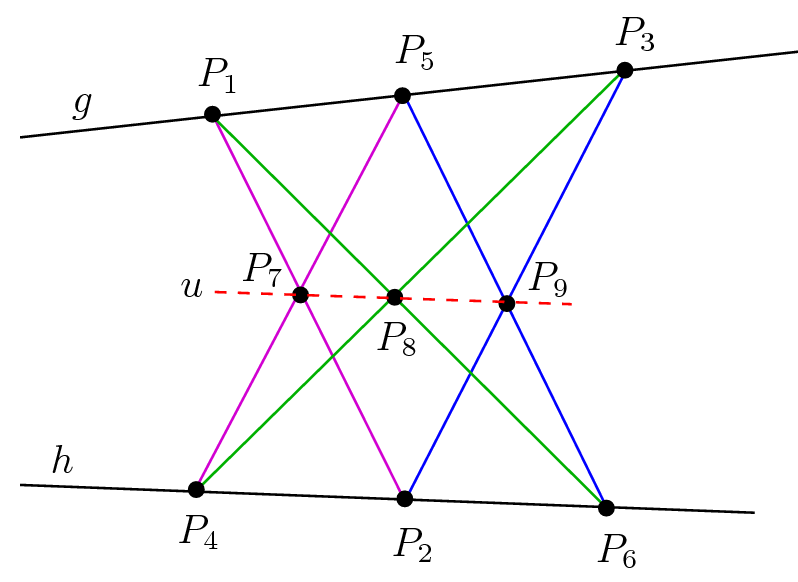
\includegraphics[width=10cm]{pics/papova_veta.png}
	\caption{Pappova věta}
	\label{obrazek:pap}
\end{figure}


Obecně lze transformaci pomocí matic zapsat:

\begin{align} \label{proj_obec}
\begin{pmatrix}
x'\\ 
y'\\ 
1
\end{pmatrix} = 
\begin{pmatrix}
a & b & c\\ 
d & e & f\\ 
g & h & 1
\end{pmatrix} 
\begin{pmatrix}
x\\ 
y\\ 
1
\end{pmatrix}
\end{align}

Po roznásobení mají rovnice tvar:


\begin{align} \label{proj_roz}
\begin{split}
x' &= \frac{ax + by + c}{gx + hy + 1} \\
y' &=\frac{dx + ey + f}{gx + hy + 1}
\end{split}
\end{align}

Následně lze přejít k vyrovnání, kterým jsou získány vyrovnané veličiny.

\section{Křivková a vyrovnávací transformace}
Křivková transformace (spline transformation) a vyrovnávací transformace (adjust transformation) při georeferencování ztotožní identické body nezávisle na jejich rozmístění. Důsledkem toho může docházet k výrazným deformacím. Křivková transformace využívá pro výpočet matematicky generované křivky, zatímco vyrovnávací transformace kombinuje polynomické transformace s interpolačními technikami. 

Více o těchto transformacích se lze dočíst v knize Jiřího Cajthamla \cite{transformace}. 






\chapter{Příprava dat}




\section{Tvorba 3D modelu Strakonického hradu}
Tvorba 3D modelu Strakonického hradu probíhala v programu SketchUp, který vyvinula americká společnost Last Software. Velkou výhodou tohoto programu je to, že umožňuje vytvořený objekt propojit s libovolným softwarem GIS a umístit jej v prostoru. 

Software SketchUp byl poprvé představen na trhu v roce 2000, kdy sklidil velké úspěchy a zájem významných firem. V tomto roce také vyhrál ocenění \textit{Best New Products or Services}. V roce 2006 je program koupen společností Google, která jej rozšiřuje a vylepšuje některé funkce. V roce 2012 je SketchUp koupen společností Trimble, která s Googlem stále spolupracuje a společně se~podílí na rozvoji služby SketchUp 3D Warehouse, která v sobě obsahuje několik existujících komponent z celého světa. Tato skutečnost umožňuje při vytváření 3D modelů používat již existující textury a objekty (stromy, dopravní značky~aj.). \cite{sketchup1} \cite{sketchup2}

\subsection{Zpracování}
Při tvorbě 3D modelu se vycházelo z půdorysu. Jednotlivé části hradu byly vytvářeny základními funkcemi programu SketchUp. Program je velmi intuitivní a uživatelsky přívětivý. Z toho důvodu, že se jedná o rozsáhlou stavbu, byl objekt značně generalizován. 

\begin{figure}[h]
	\centering
	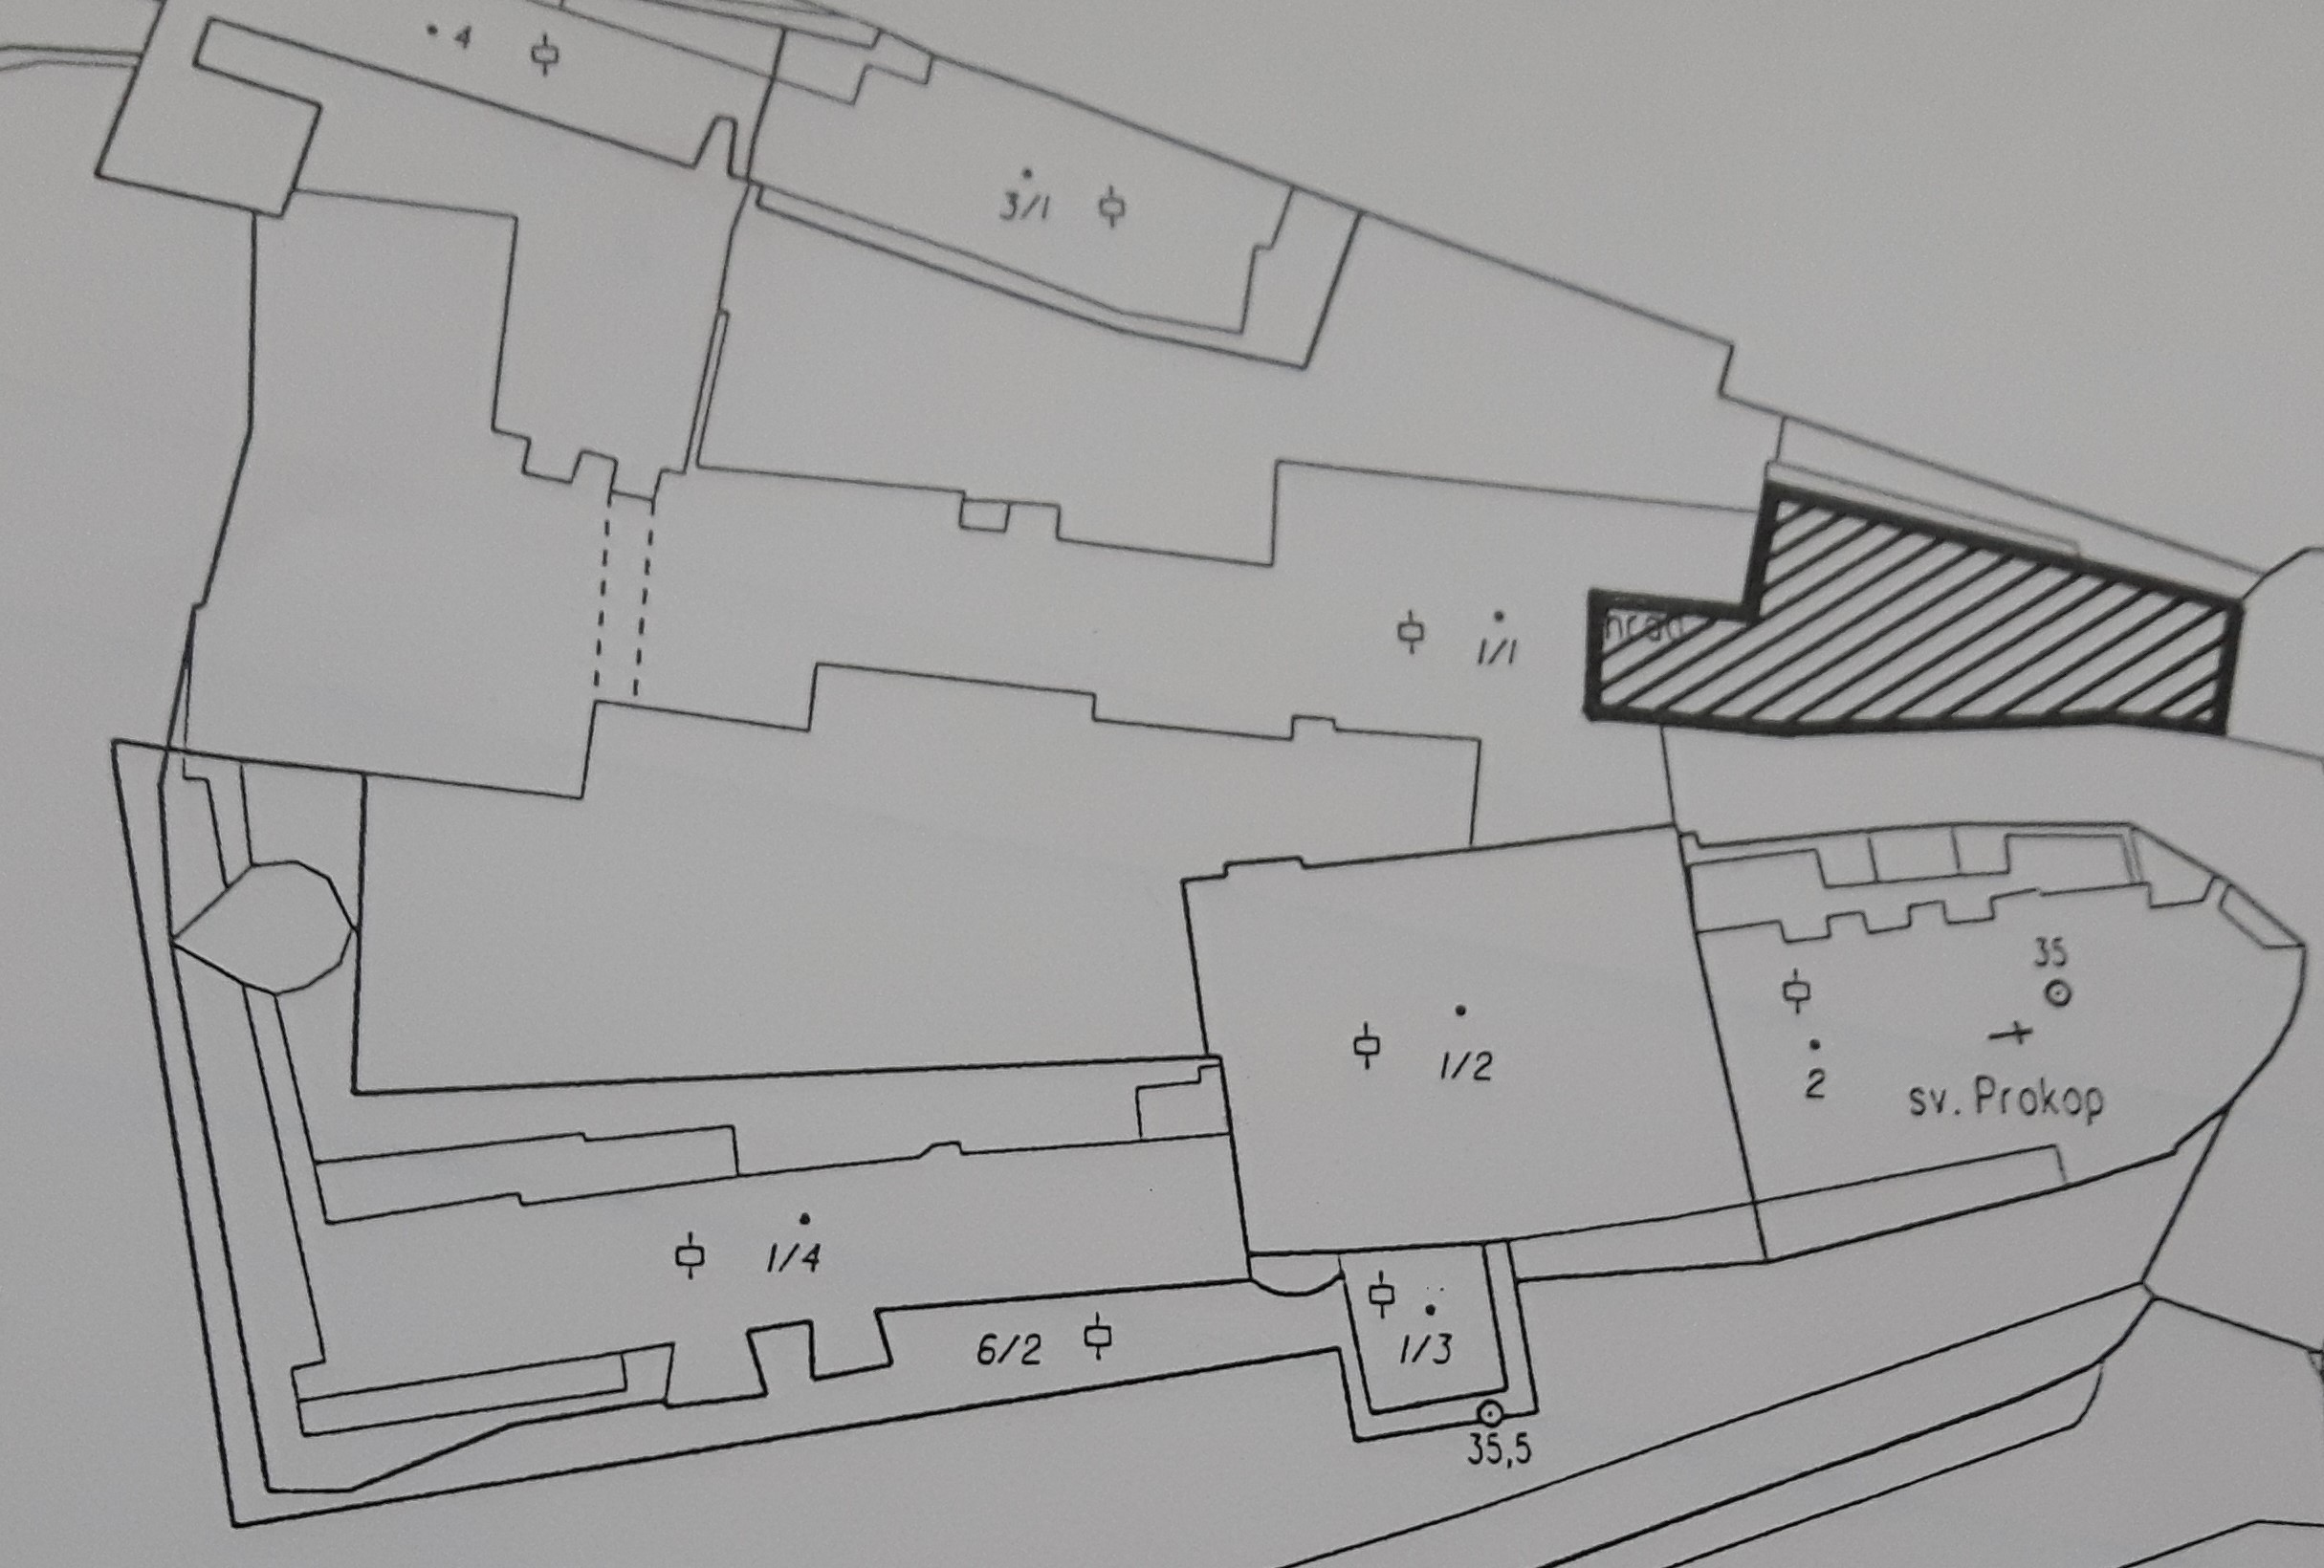
\includegraphics[width=13cm]{pics/pudorys_hrad.jpg}
	\caption{Půdorys Strakonického hradu}
	\label{obrazek:pudorys}
\end{figure}

Dílčí části Strakonického hradu byly vytvářeny lomenými čarami a oblouky. Z toho důvodu, že se nejedná o stěžejní část této práce, nebyly detailněji vyhotoveny některé části objektu a místo toho byly vloženy textury, které tyto objekty již obsahují. Při volbě textur se vycházelo z fotografií pořízených autorkou. Fotografování za účelem získání textur a lepší představy při samotném modelování bylo prováděno v období od ledna do května roku 2019. 

Fotografování v tomto poměrně velkém časovém rozmezí bylo zapřičiněno z~několika důvodů. Hlavní vliv na fotografování měly restaurátorské práce, neboť je hrad v rozsáhlé rekonstrukci. Dalším činitelem bylo počasí a povětrnostní podmínky. V neposlední řadě má vliv i časové období, kdy je fotografování prováděno. U částí hradu, kde je znatelná vegetace, bylo fotografování upřednostněno v době hlavního vegetačního období.

Velká výhoda softwaru SketchUp je ta, že lze projekt geolokalizovat. Geolokalizace vzniká jednoduchou volbou \textit{File $\rightarrow$ Geo-location $\rightarrow$ Add \mbox{location ... }}. Model byl publikován na webovou stránku 3D Warehouse pomocí volby funkce \textit{File $\rightarrow$ 3D Warehouse $\rightarrow$ Share Model ... }. Zároveň byla vytvořena krátka animace, ve~které byla snaha zachytit model z několika různých pohledů. Tato animace je součástí příloh a byla publikována na server YouTube, který v~současné době spadá také pod společnost Google a prezentuje se jako dceřiná společnost této firmy. 

Při zpracování byla nejprve v modelu vytvořena gotická věž Rumpál (obr. č.~\ref{obrazek:sk1}), která je nejspíš nejvýraznější ikona hradu. Následně bylo vymodelováno II. hlavní nádvoří (obr. č. \ref{obrazek:sk2}). Poté byl vytvořen kostel sv. Prokopa s ním související I. hlavní nádvoří (obr. č. \ref{obrazek:sk3}). Na obrázku č. \ref{obrazek:sk4} lze vidět výsledný model, na obrázku č. \ref{obrazek:sk5} je zobrazen tento model včetně textur. Na obrázku č. \ref{obrazek:sk6} je již finální podoba hradu se všemi detaily.

\begin{figure}[h]
	\centering
	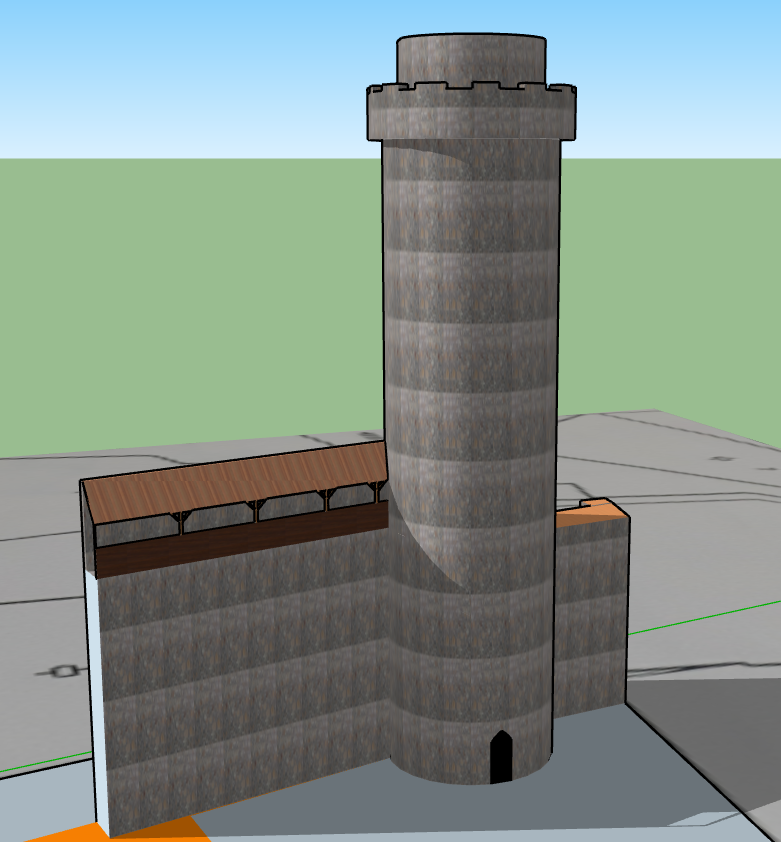
\includegraphics[width=5cm]{pics/sketchup1.png}
	\caption{Gotická věž Rumpál}
	\label{obrazek:sk1}
\end{figure}

\begin{figure}[h]
	\centering
	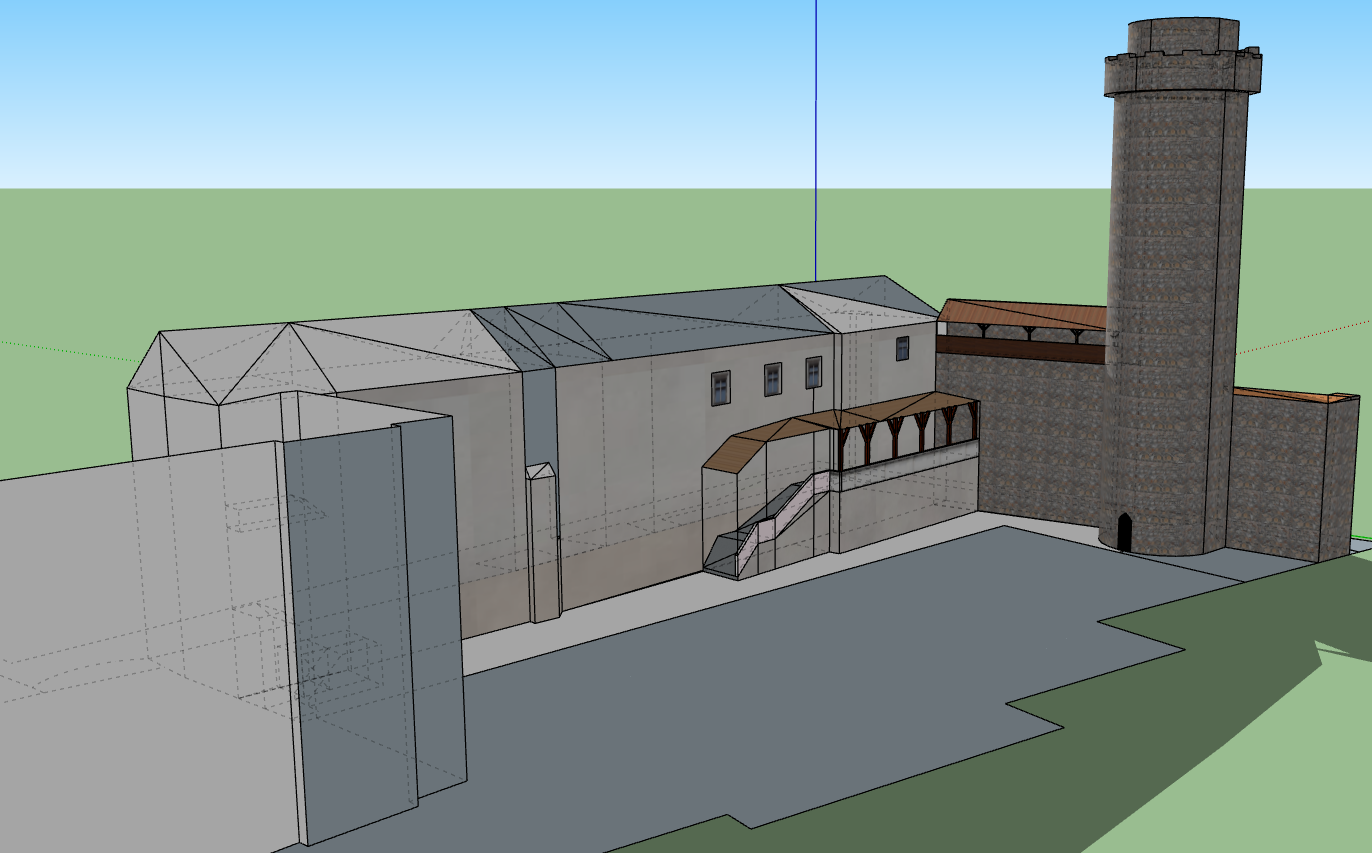
\includegraphics[width=8cm]{pics/sketchup2.png}
	\caption{II. hlavní nádvoří Strakonického hradu}
	\label{obrazek:sk2}
\end{figure}

\begin{figure}[h]
	\centering
	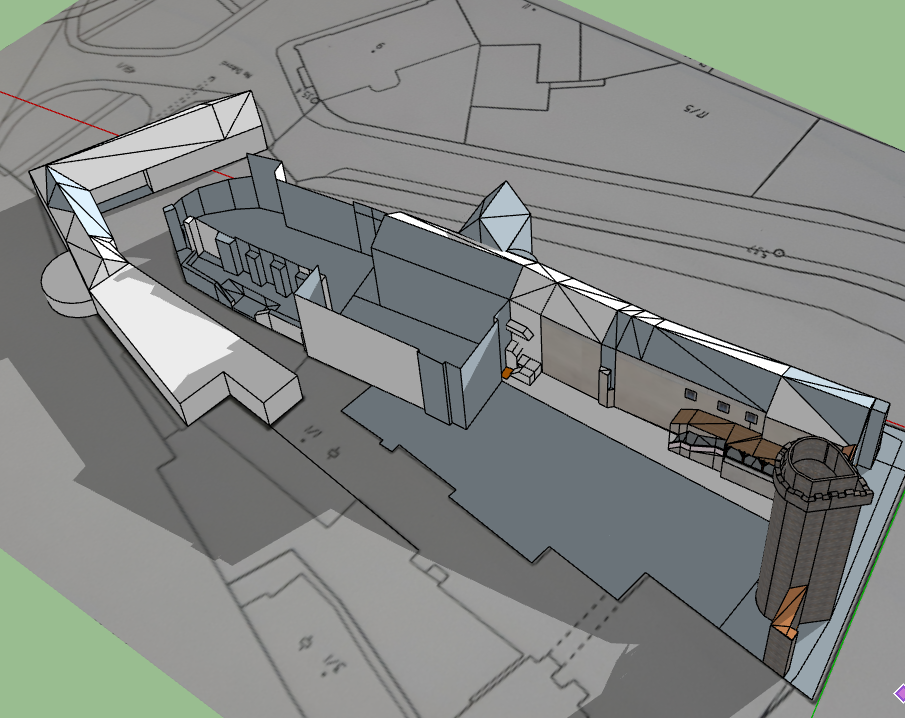
\includegraphics[width=8cm]{pics/sketchup3.png}
	\caption{I. hradní nádvoří a kostel sv. Prokopa}
	\label{obrazek:sk3}
\end{figure}

\begin{figure}[h]
	\centering
	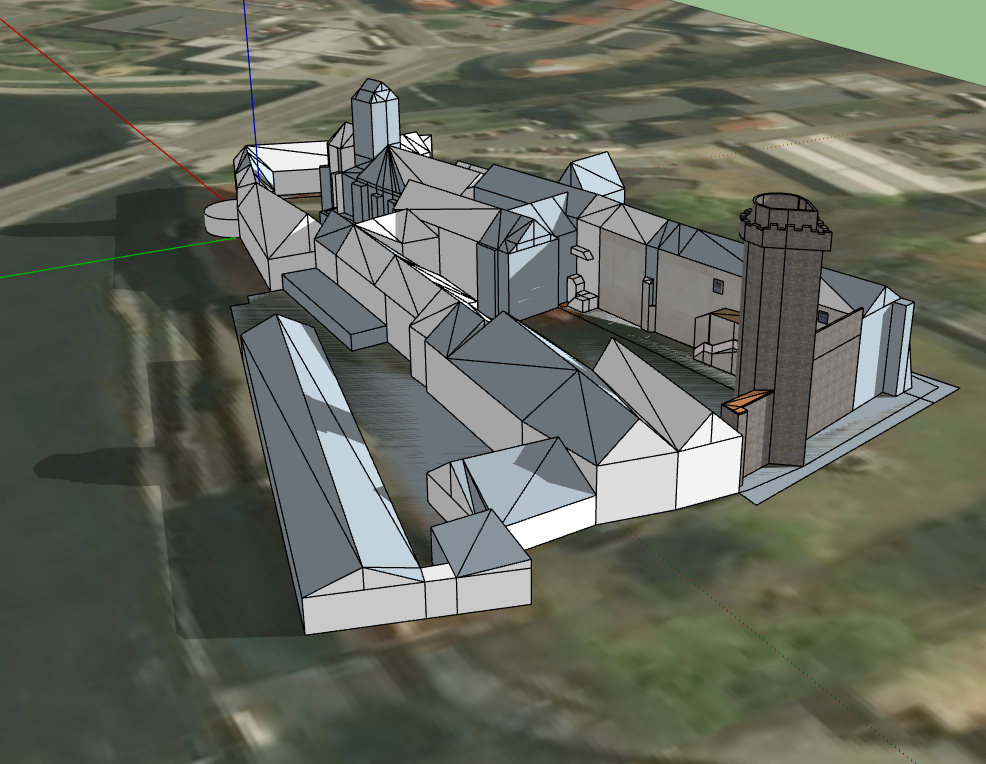
\includegraphics[width=8cm]{pics/sketchup4.png}
	\caption{Vytvořený model hradu}
	\label{obrazek:sk4}
\end{figure}

\begin{figure}[h]
	\centering
	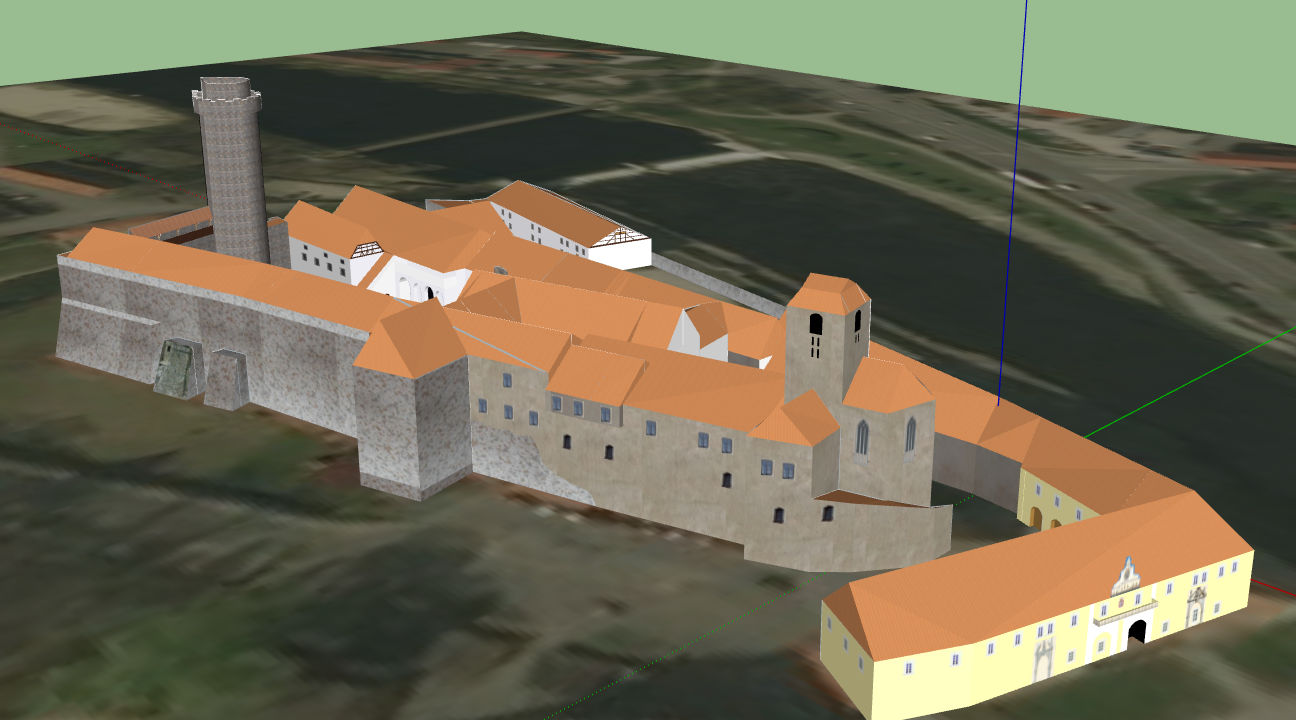
\includegraphics[width=8cm]{pics/sketchup5.png}
	\caption{Model Strakonického hradu doplněný o textury}
	\label{obrazek:sk5}
\end{figure}

\begin{figure}[h]
	\centering
	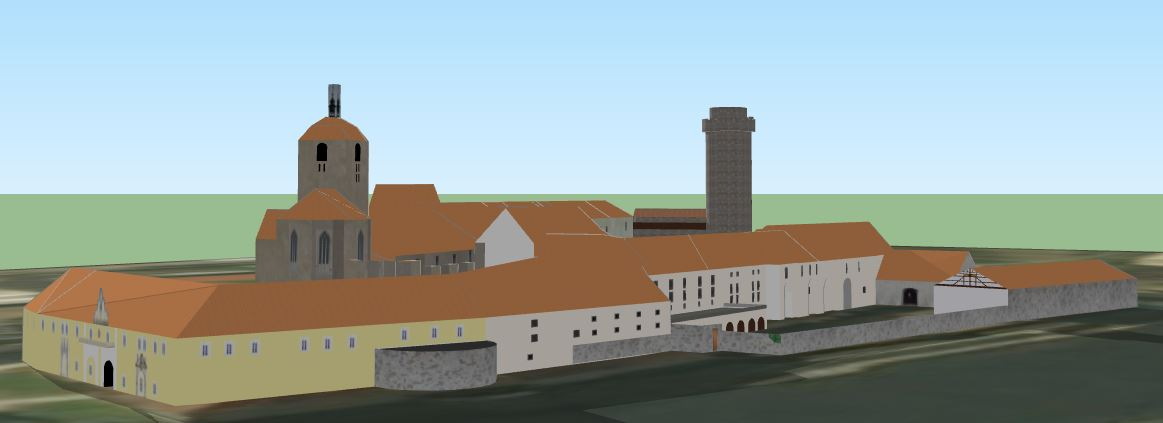
\includegraphics[width=13cm]{pics/final_model.jpg}
	\caption{Výsledný 3D model Strakonického hradu}
	\label{obrazek:sk6}
\end{figure}

\clearpage

\subsection{Prezentace výsledků z programu SketchUp}
Výsledný model byl publikován na stránku 3D Warehouse, která slouží jako úložiště modelů vytvořených v programu SketchUp a jejich sdílení se všemi uživateli internetu. V rámci stránky lze vyhledat a následně stáhnout do svého projektu již vytvořený libovolný objekt. 3D Warehouse v současné době nabízí možnost volby z několika různorodých kategorií, kromě stavebních objektů je možné stáhnout model zvířat, lidí, nábytku či jídla. 

SketchUp nabízí i možnost tvorby animace modelu, kdy jsou postupně voleny jednotlivé scény a program z nich vytvoří krátké video. Model je rozsáhlý a při nasnímání hradu ze všech významných pohledů vzniklo video o 40~scénách. Takto obsáhlé video nešlo publikovat ve formátu \textit{avi}, bylo tedy vytvořeno ve formátu \textit{mp4}. Zároveň byla vytvořena i kratší animace, která byla exportována ve formátu \textit{avi}. Vzniklá videa byla nahrána na server YouTube, kde jsou volně ke zhlédnutí. 


\section{Zpracování kartografických podkladů}
Zpracování kartografických podkladů probíhalo v softwaru ArcGIS od společnosti ESRI, která se zabývá vývojem softwaru pro práci s geografickými informačními systémy. Zakladatelem společnosti byl Jack Dangermond. ArcGIS je primárně určen pro práci s prostorovými daty, jejich tvorbu, správu či~analýzu.

Před samotným zpracováním byla zapotřebí příprava prostředí a mapového okna v programu ArcMap. Nejprve byla vytvořena geodatabáze \textit{Otava.gdb}. Geodatabáze je interní formát společnosti ESRI, který slouží k ukládání a~manipulaci s prostorovými daty. Velkou výhodou je to, že všechny soubory jsou uloženy v jednom adresáři. Pro geodatabázi lze nastavit i defaultní souřadnicový systém, pro databázi \textit{Otava.gdb} byl zvolen S-JTSK Krovak East North (EPSG: 5514).

Pro mapový dokument byla zvolena možnost ukládání relativní cesty zdrojových dat. Relativní cesta byla nastavena z toho důvodu, že zpracování probíhalo na více počítačích. 


\subsection{Georeferencování}

Císařské povinné otisky map stabilního katastru a Státní mapa 1 : 5 000 – odvozená byly zapůjčeny od Českého úřadu zeměměřického a katastrálního ve~formátu JPG ve formě rastrových dat. Tato data bylo nutné zgeoreferencovat\footnote{Proces umístění rastru do známého souřadnicového systému} za~využití znalosti transformace. 

Pro georeferencování posloužila jako podkladová data katastrální mapy, jež jsou k dispozici online prostřednictvím WMS služby poskytnuté ze serveru ČÚZK.  Jako vlícovací body byly u prvního rastru voleny přednostně takové body, u kterých se předpokládá již zmíněná stabilita a neměnnost. U~dalších rastrů byly vlícovací body voleny s ohledem na klad mapových listů a~plynulou návaznost se sousedními rastry. Vzhledem k měřítku mapových podkladů byl požadavek na maximální hodnotu směrodatné odchylky 2,5 m. Pro kvalitněji zgeoreferencovaná data byly vlícovací body voleny rovnoměrně rozmístěné po~celém rastru a byla snaha o dosažení nadbytečného množství, aby při transformaci docházelo k vyrovnání MNČ. 


\subsection{Tvorba mozaiky}
Zpracovaná data bylo potřeba vhodně uložit a zobrazit jako celek. Za tímto účelem byl v geodatabázi vytvořen nový objekt – mozaika. Zgeoreferencované listy byly následně do mozaiky nahrávány funkcí \textit{Add Raster To Mosaic Dataset}.

Vzhledem k tomu, že každý z použitých mapových podkladů obsahoval mimorámové údaje, bylo nutné rastry oříznout. Za tímto účelem byla v rámci geodatabáze vytvořena polygonová vrstva. V této vrstvě byl pro každý mapový podklad vytvořen maskovací polygon, který přesně ohraničuje oblast z každého listu. Polygon byl pojmenován podle daného rastru, toto označení je dále využito jako propojovací klíč. 

Pro přiřazení ořezového polygonu ke konkrétnímu rastru byla v rámci mozaiky použita funkce \textit{Modify/Import Footprints or Boundary}, v níž byla definována polygonová vrstva a propojovací klíč. Výsledné hranice zgeoreferencovaných listů lze vidět na obrázku č. \ref{obrazek:CPO_viz}. 


\begin{figure}[h]
	\centering
	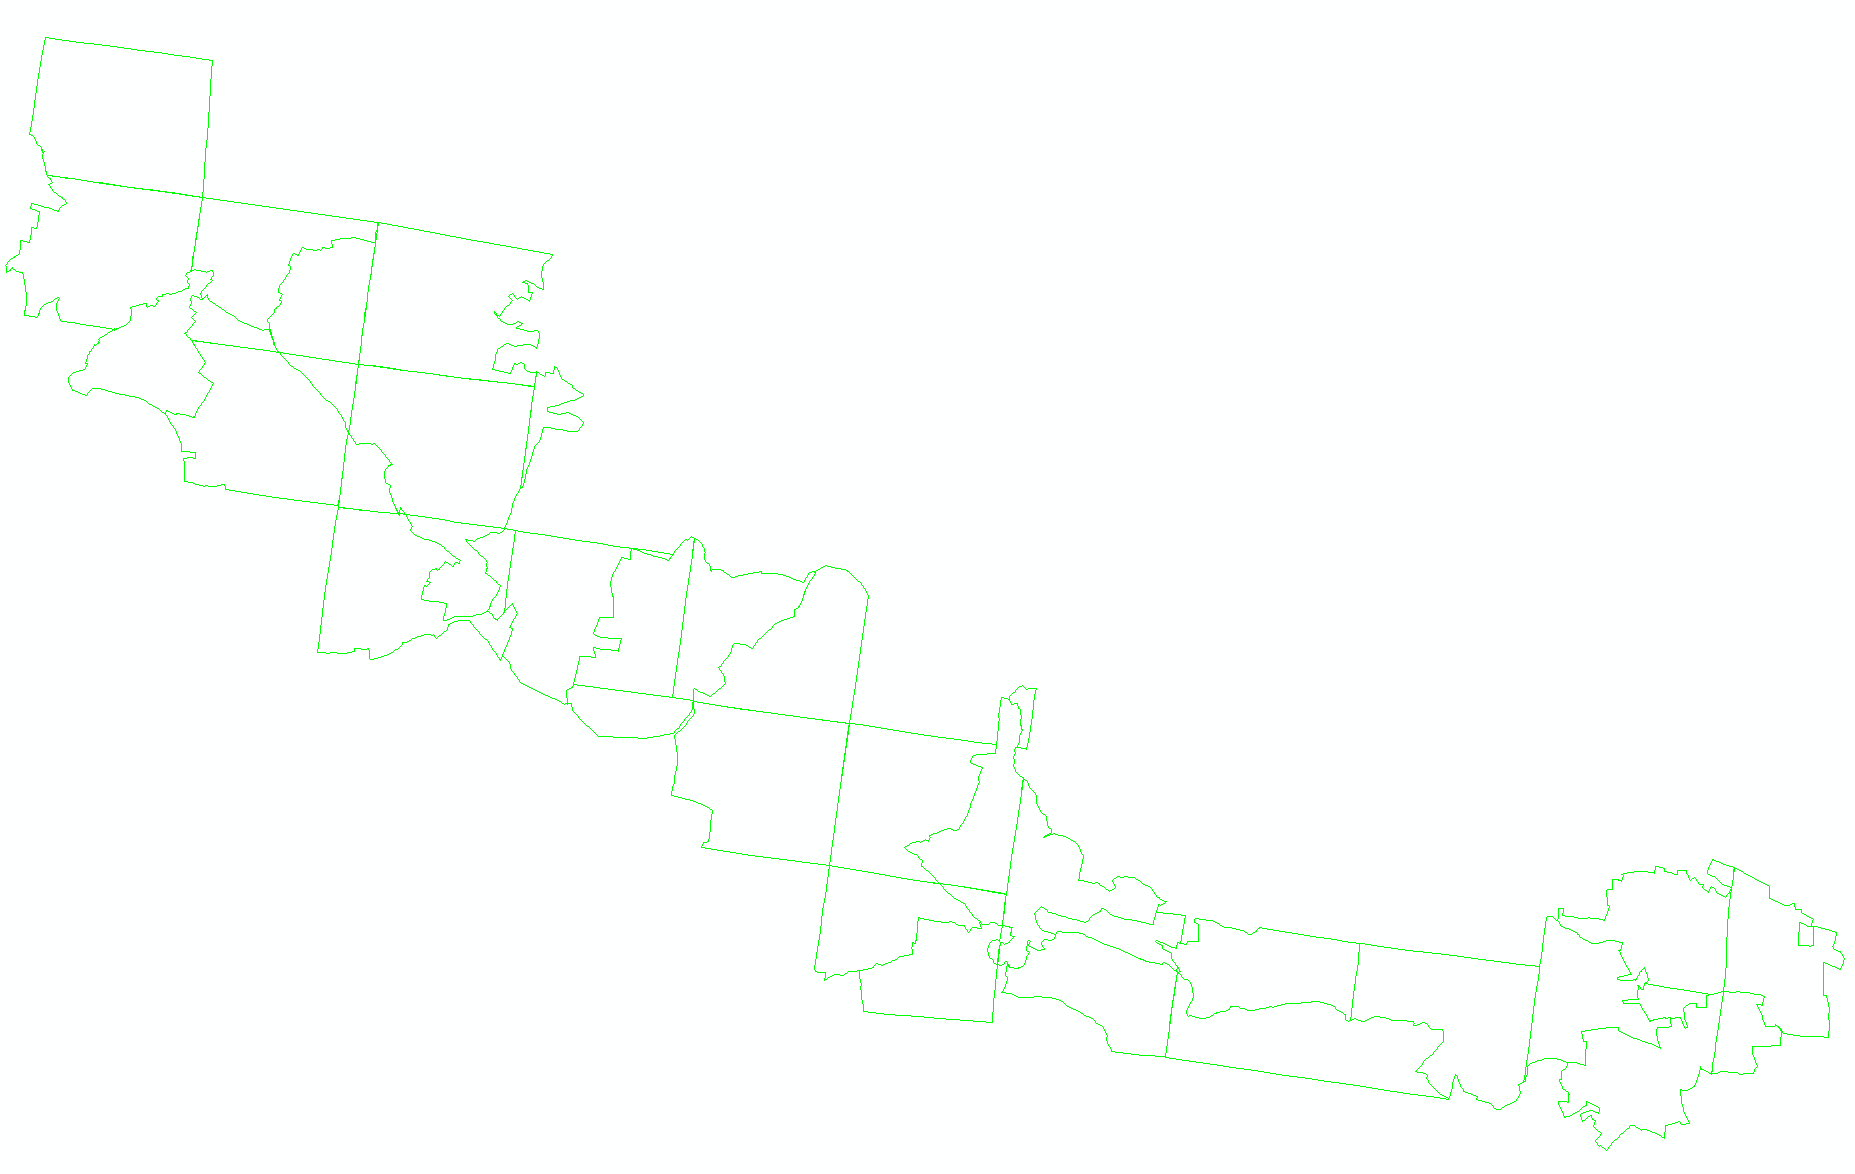
\includegraphics[width=17cm]{pics/klad_CPO.png}
	\caption{Hranice zgeoreferencovaných listů CPO}
	\label{obrazek:CPO_viz}
\end{figure}

\subsection{Vektorizace}
Pro následné zpracování byly vybrané objekty z map CPO zvektorizovány, což znamená, že byly převedeny z rastru na vektor. Vektorizace byla prováděna ručně a byly vektorizovány budovy, které byly dále rozdělovány na spalné a~nespalné, lesy a řeka. 

Pro vektorizaci byly vytvořeny nové polygonové vrstvy, do nichž byly objekty ukládány. Tvorba objektů probíhala za pomoci funkce \textit{Create Features} v~liště \textit{Editor}. 


\section{Modelování krajiny}
Základ pro modelování byl vytvořen v programu ArcMap, následné zpracování probíhalo v softwaru ArcGIS Pro. Do funkce pro vymodelování krajiny byly na~vstupu výškové kóty, vrstevnice a břehová čára.

\subsection{Vektorizace vrstevnic}
Vrstevnice pro tvorbu 3D modelu byly převzaty z SMO–5. Před samotnou tvorbou bylo nutné rastry samostatně zpracovat, neboť pro vektorizaci sloužila nadstavba ArcScan, která dokáže pracovat pouze s rastry, které jsou definovány právě dvěma barvami. 

Pro zpracování rastrů posloužil program IrfanView, který je nejčastěji využíván k prohlížení obrázků, zvuků či videa. Program je pro nekomerční účely ke~stažení zdarma. Podporuje velké množství grafických formátů, není paměťově náročný, dokáže měnit počet barev a přebarvovat grafické vstupy a~umožňuje konverzi rastrů. Program byl přeložen do několika jazyků, včetně češtiny. 

Při přebarvení byla zkopírována složka se zgeoreferencovanými SMO–5 a~ty byly poté upraveny pro vektorizaci. Nejprve byla snížena barevná hloubka na~16 barev, aby při volbě barvy byl sejmut odstín vrstevnic. Funkcí \textit{Replace Color – Replace source color} byly ručně vybírány pixely znázorňující vrstevnice, které byly následně přebarveny na růžovou, aby byl výrazný kontrast se zbylými pixely rastru. Poté byla snížena barevná hloubka na 2 bity, čímž vznikl černobílý rastr. 

\begin{figure}[h]
	\centering
	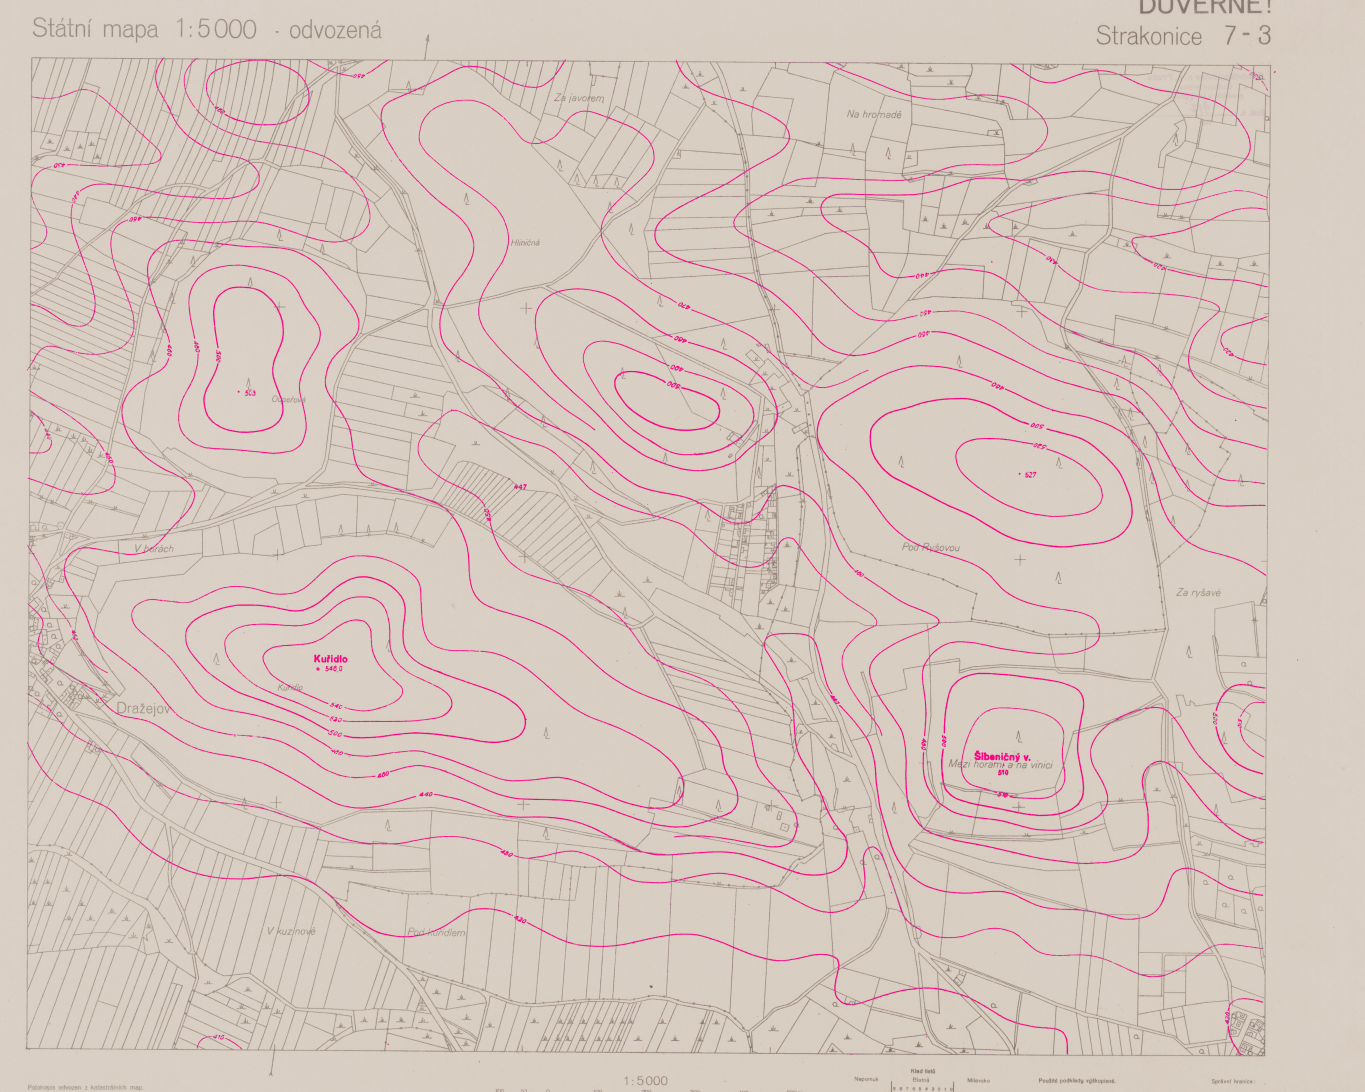
\includegraphics[width=8cm]{pics/vrstevnice.png}
	\caption{Předpřipravený přebarvený rastr pro vektorizaci}
	\label{obrazek:vrstevniceruzova}
\end{figure}

\begin{figure}[h]
	\centering
	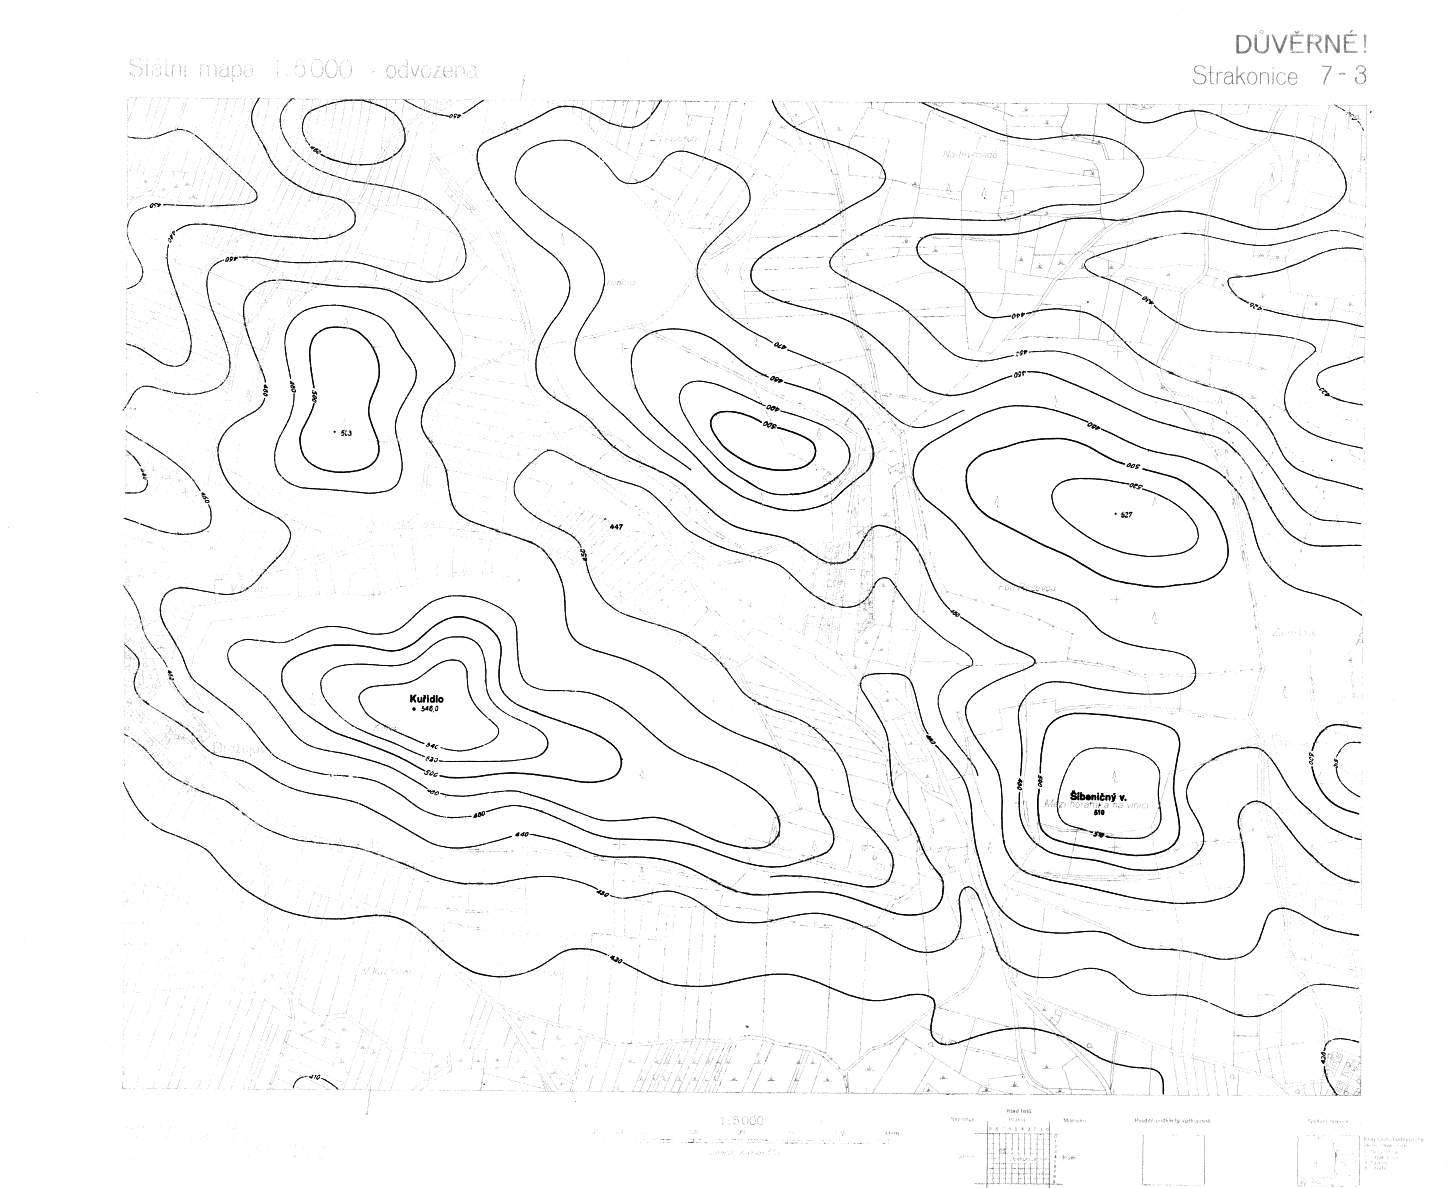
\includegraphics[width=8cm]{pics/vrstevnice2.png}
	\caption{Zpracovaný 2bitový rastr}
	\label{obrazek:vrstevnice2bit}
\end{figure}

Tím, že byly používány soubory vzniklé při georeferencování, nebylo zapotřebí tyto rastry opětovně georeferencovat. Rastry načtené v ArcMapu byly reklasifikovány na 2 hodnoty – bílá a černá. Před zpracováním je nutné aktivovat nadstavbu ArcScan. Aktivace se nachází pod volbou \textit{Customize – Extenstions}. Zároveň byla vytvořena liniová vrstva se dvěma atributy, nadmořskou výškou a délkou. 


Při spuštění nadstavby ArcScan je možnost smazání nežádoucích objektů (tiráž, chybné přebarvení atd.). K tomu slouží funkce \textit{Raster Cleanup}. Funkce nabízí mnoho možností jak zpracovat rastr v prostředí ArcGIS. V této práci byla použita pouze možnost \textit{Guma}, při níž byly nežádoucí prvky vymazány. 

ArcScan nabízí 3 možnosti vektorizace, a to ruční, automatickou a poloautomatickou. Nejprve byla vyzkoušena automatická vektorizace. Při automatické vektorizaci bylo nutné nastavit parametry vektorizace (maximální tloušťku linie, míru vyhlazení, metodu řešení průsečíků, atd.) a zvolit barvu vrstvy. Zároveň bylo možné nastavit i styl generování vrstevnic, ten byl zvolen \textit{Contour}. Pro vyhledání optimálního výsledku byly parametry několikrát měněny. Přesto nebyl výsledek dostačující, mezi vrstevnicemi byly často mezery a zvektorizovaly se i objekty, které bylo následně nutné vymazat. 

Z důvodu nespokojenosti s automatickou tvorbou byla vyzkoušena poloautomatická tvorba vrstevnic. Pro poloautomatickou tvorbu byla použita funkce \textit{Vectorization Trace}, která dokáže rozpoznat buňky, které na sebe navazují a~vytvoří z nich linii. Poloautomatická tvorba probíhala současně s ruční, neboť na některých místech docházelo k tomu, že nenavazovala žádná buňka a bylo zapotřebí ručně přichytit linii na buňky, v jejichž směru vrstevnice pokračovala.

Po vektorizaci vrstevnic byla vytvořena bodová vrstva obsahující výškové kóty. Kóty byly přejímány z SMO–5 spolu s výškami. Zároveň byla vytvořena liniová vrstva \textit{brehovka}, do níž byl zvektorizován břeh řeky s odhadem nadmořské výšky.



\subsection{Topo to raster}
Funkcí \textit{Topo to raster} byla vytvořena barevná hypsometrie zadaného území. Do funkce vstupovala vrstva s výškovými kóty (\textit{PointElevation}), vrstevnice (\textit{Contour}), ohraničující polygon pro modelování (\textit{Boundary}) a břehovka (\textit{Contour}). Funkce nabízí mnoho dalších vstupů, je zde možnost nahrání vodního toku, útesu či pobřeží. Při modelování bylo vyzkoušeno několik různorodých vstupních dat, přesto zmíněný způsob se jevil jako nejsprávnější a téměř bezchybný. 

\subsection{3D model krajiny}
V programu ArcMap lze pro přibližnou představu vygenerovat stínovaný povrch terénu pomocí funkce \textit{Hillshade}. Pro tvorbu 3D modelu posloužil program ArcGIS Pro. Jedná se o nově vytvořený software, jehož hlavním cílem je zjednodušení práce. Narozdíl od ArcMap umožňuje v rámci aplikace pracovat s~několika mapovými okny současně. 

V softwaru ArcGIS Pro byla vytvořena lokální scéna, do níž byla nahrána vrstva vzniklá funkcí \textit{Topo to raster}. Tato vrstva nahradila defaultní vrstvu v záložce \textit{Elevation Surfaces}, díky čemuž bylo možné vizualizovat vytvořený model krajiny. Do programu byla nahrána i polygonová vrstva řeky a mozaika s georeferencovanými rastry SMO–5. Na obrázku č. \ref{obrazek:otava_knezihora} lze vidět ukázku vizualizace vytvořeného 3D modelu.

\begin{figure}[h]
	\centering
	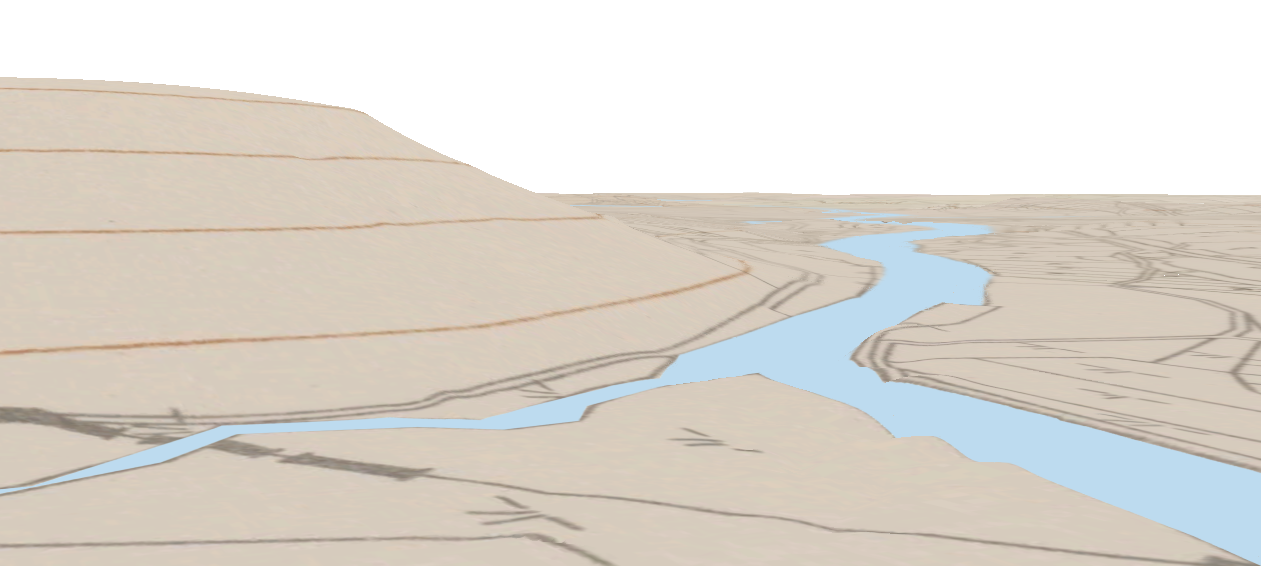
\includegraphics[width=10cm]{pics/arcgispro.png}
	\caption{Vizualizace krajiny v softwaru ArcGIS Pro}
	\label{obrazek:otava_knezihora}
\end{figure}

\section{Procedurální modelování}
Jedná se o automatický způsob vytváření 3D modelů. Jednotlivé objekty jsou generovány z jednoduchých komponent dle předepsaných pravidel. Například model stromu má komponenty listy a větve, pravidla definují geometrii rozvětvování a parametry obsahují informace o hustotě listů, maximální tloušťce větve apod. Tímto způsobem lze pro stromy definovat různá pravidla a předpisy, čímž lze docílit toho, že vzniknou různorodé druhy stromů a na vytvořeném polygonu bude vygenerován les. \cite{jaderka}

\subsection{CityEngine}
CityEngine vytvořil Pascal Müller. V roce 2011 jej odkoupila společnost Esri, která program přejmenovala na Esri CityEngine. Jedná se o software, který umožňuje z 2D geografických dat vytvořit 3D simulaci. Program podporuje mnoho formátů, včetně geodatabáze ArcGIS. Vytvořený model je možné publikovat a sdílet prostřednictvím ArcGIS Online. \cite{arcdata}

\subsection{Modelování}
Pro modelování v programu CityEngine byl založen projekt. Tento projekt má defaultně nastavené složky (assets, data, maps, models, rules, scenes, scripts). Před samotnou tvorbou bylo nutné nahrát do složky \textit{assets} textury a~do~složky \textit{rules} pravidla pro procedurální modelování, která sestavil Pavel Tobiáš. Do~složky \textit{maps} byl vložen rastr vytvořený v programu ArcMap funkcí \textit{Topo to~raster}. Do složky \textit{data} byly importovány zvektorizované shapefily a~do~složky \textit{models} byl vložen generalizovaný 3D model Strakonického hradu.

Při importu modelu nabízí CityEngine několik různých formátů, ve kterých lze model nahrát. Vzhledem k tomu, že se jedná o velký a členitý objekt, docházelo při nahrání k mnoha komplikacím. Nejvýraznější komplikace byla s~texturami, které v některých formátech zcela chyběly či se zobrazily na jiných místech. Nejkvalitněji byl model zobrazen po importu ve formátu \textit{KMZ}, kde ačkoliv není i po několika úpravách vykreslena textura Rumpálu, je vizualizace modelu v CE nejuspokojivější. 

\begin{figure}[h]
	\centering
	\includegraphics[width=13cm]{pics/hrad_ce.jpg}
	\caption{Strakonický hrad v prostředí CityEngine ve formátu KMZ}
	\label{obrazek:hradCE}
\end{figure}

\begin{figure}[h]
	\centering
	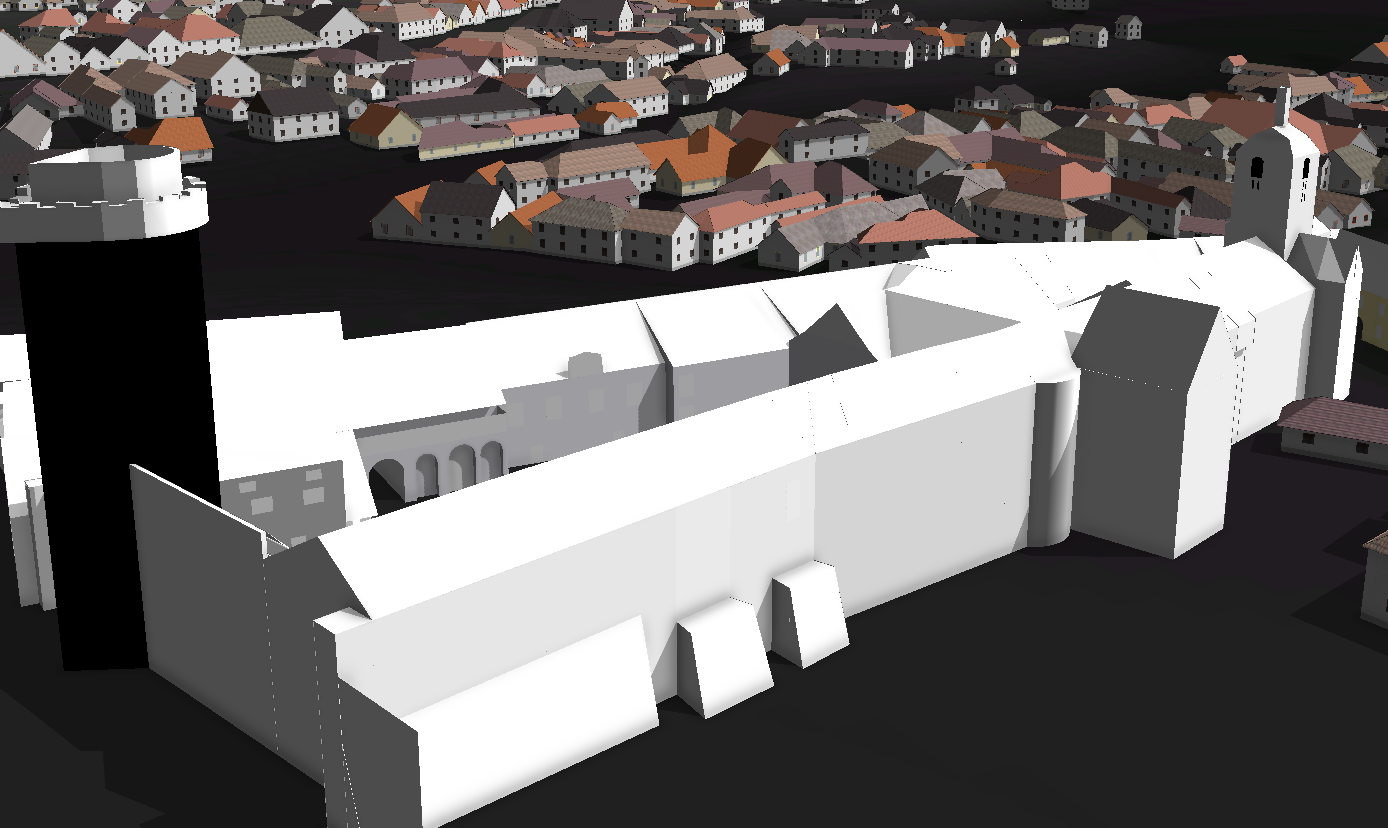
\includegraphics[width=10cm]{pics/dae.png}
	\caption{Strakonický hrad v prostředí CityEngine ve formátu DAE}
	\label{obrazek:hraddae}
\end{figure}


U nahraných vektorizovaných vrstev bylo potřeba provést drobné úpravy, neboť při generování stromů byl na polygonu lesu vždy vytvořen pouze jeden strom. V programu ArcMap byly funkcí \textit{Create Random Points} vygenerovány náhodné body s minimálním rozestupem 5 m. 

Pro následné modelování byly k jednotlivým vrstvám přiřazeny soubory s pravidly. Vygenerované objekty byly funkcí \textit{Allign shapes to terrain} umístěny na terén, čímž se zabránilo tomu, aby se objekty vznášely ve vzduchu. Vytvořené modely byly na závěr publikovány prostřednictvím ArcGIS Online.

\begin{figure}[h]
	\centering
	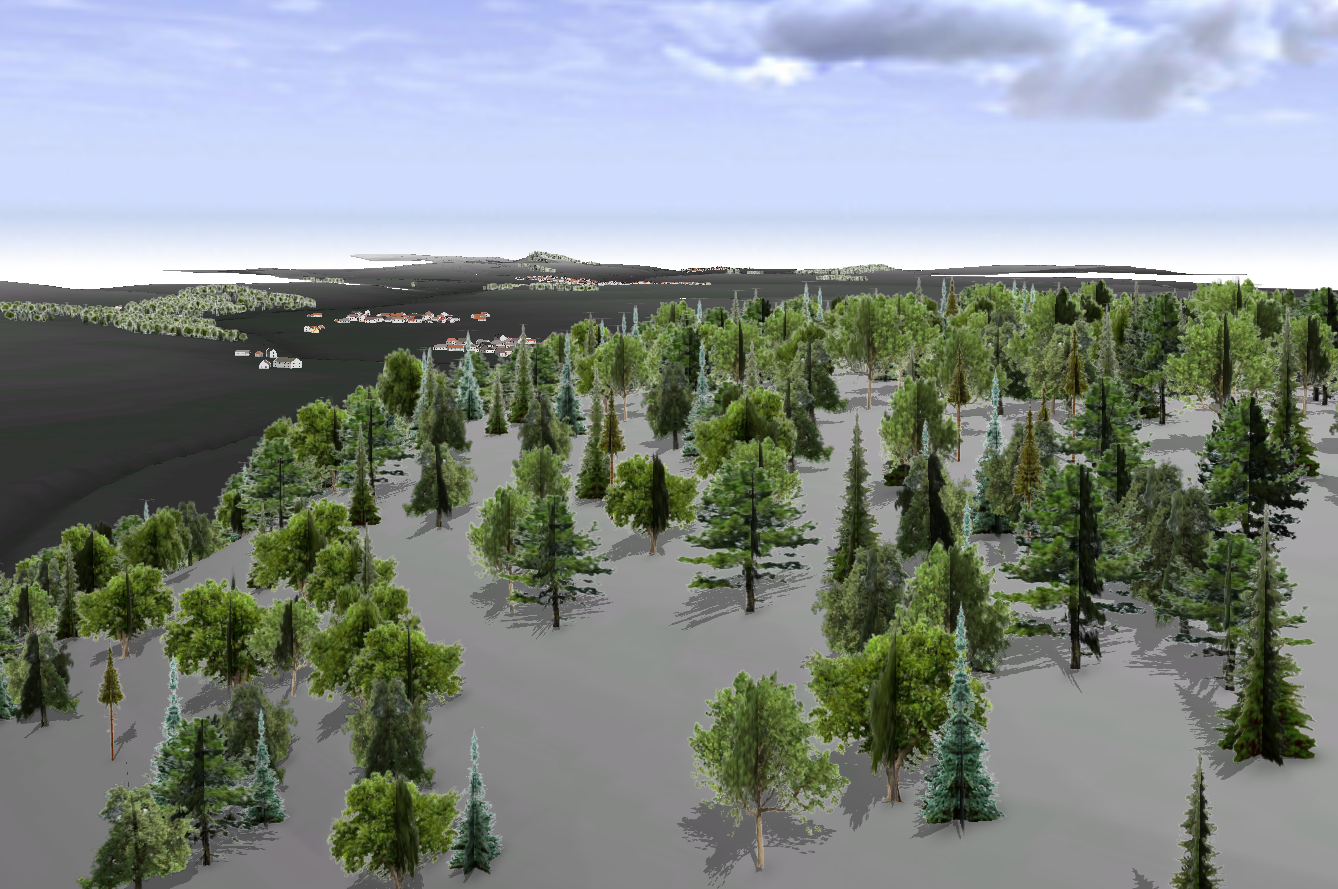
\includegraphics[width=10cm]{pics/lesy_knezihora.png}
	\caption{Vygenerovaný les - Kněží hora u Katovic}
	\label{obrazek:knezihora}
\end{figure}


\section{Publikování výsledků na internetu}
Vytvořené modely, mozaiky a vybrané vrstvy byly publikovány na server Arc\-GIS Online, odkud byla následně vytvořena webová mapová aplikace. Sdílení probíhalo funkcí \textit{Share as service}. Byla vytvořena 2D mapová aplikace a~3D~mapová aplikace. 

2D mapová aplikace obsahuje vrstvu s rastry povinných císařských otisků a~SMO–5. Zároveň byla vytvořena bodová vrstva obsahující fotografie různých míst. Mapová aplikace byla doplněna o možnost volby podkladových map, sdílení, měření vzdálenosti a tisku mapy. 

3D mapová aplikace obsahuje exportované modely z programu CityEngine, generalizovaný model Strakonického hradu a podkladovou vrstvu císařských povinných otisků. Aplikace je rozšířena o widgety s možností volby podkladové mapy, sdílení aplikace, měření vzdálenosti a tisku mapy.



\section{Porovnání výškopisu}
V rámci práce byl vytvořený model krajiny porovnáván s produktem od ČÚZK DMR 5G. DMR 5G byl získán z prohlížecí služby Esri ArcGIS Server \cite{dmr}, z níž byl pro danou oblast vyexportován ve formátu \textit{TIFF}. Vyexportovaný soubor byl následně v programu ArcMap oříznut přesnou hranicí oblasti funkcí \textit{Extract by mask}. 

Vytvořený rastr modelu krajiny a oříznutý rastr DMR 5G byly mezi sebou porovnány funkcí \textit{Raster Calculator}. Do funkce byl vložen rozdíl vytvořeného povrchu a staženého povrchu. Výsledný rastr znázorňoval rozdíl obou výšek. Rastr s rozdílem je součástí příloh. Na obrázku č.~\ref{obrazek:histogram} lze vidět histogram rozdílů. Maximální rozdíly byly 36 m, tato výrazná výchylka je zřejmě způsobena místy, kde nebyla k dispozici data. Z histogramu je patrné normální rozdělení a průměrný rozdíl 1 m. Lze tedy vytvořený model krajiny považovat za kvalitní. 

\begin{figure}[h]
	\centering
	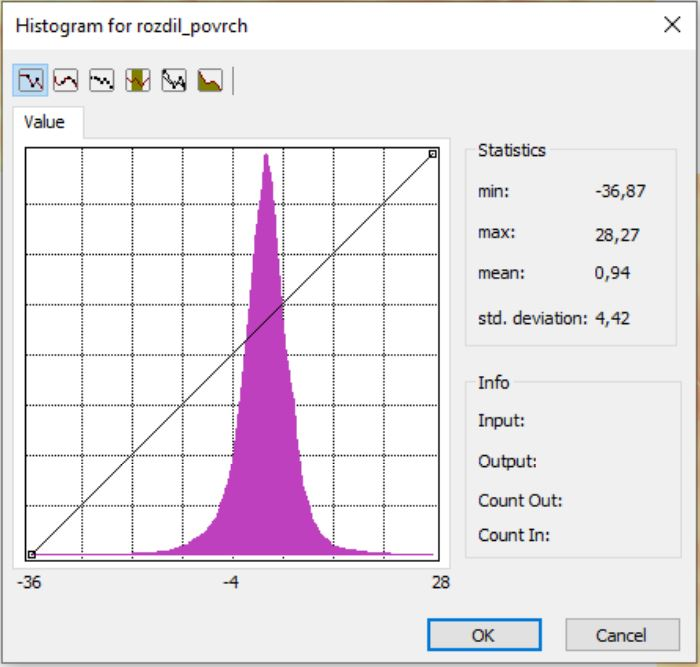
\includegraphics[width=8cm]{pics/histogram.jpg}
	\caption{Histogram rozdílu nadmořských výšek}
	\label{obrazek:histogram}
\end{figure}

Oba modely byly také porovnávány vizuálně mezi sebou. Dle obrázku č.~\ref{obrazek:rozdilvysek} je patrné, že až na výjimky jsou modely téměř totožné. 

\begin{figure}[htp]
\centering
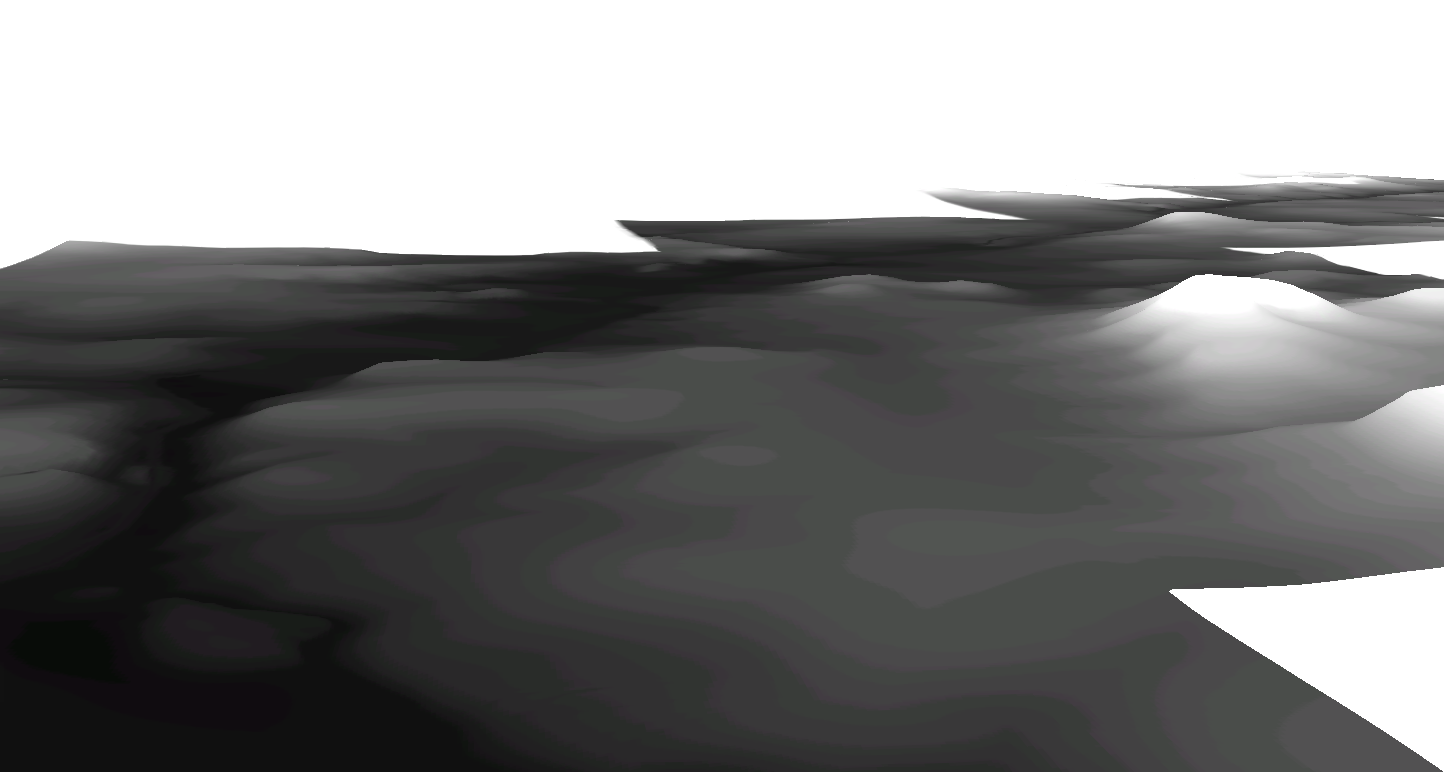
\includegraphics[width=6cm]{pics/dm_smo5.png}
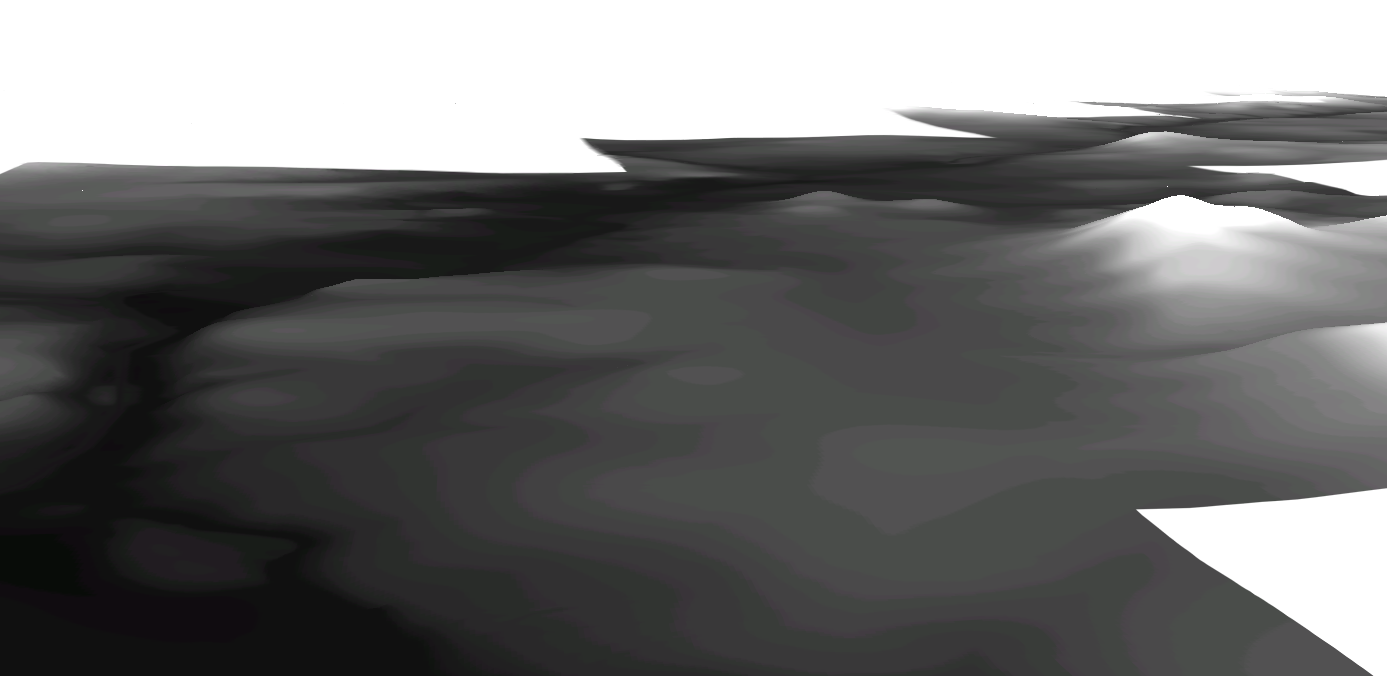
\includegraphics[width=6cm]{pics/dmr_5g.png}
\caption{Vlevo model krajiny vytvořený z dat SMO–5, vpravo DMR 5G}
\label{obrazek:rozdilvysek}
\end{figure}


\chapter{Prezentace na webových stránkách}
I přes znalost značkovacího jazyka HTML byla webová stránka vytvářena online přes stránku Wix. Stránka Wix nabízí možnost bezplatného webhostingu, případně placené verze, pokud uživatel nechce na svých webových stránkách zobrazit reklamy či chce využít jiných prémiových služeb. Velkou výhodou tohoto webu je interaktivní tvorba, která umožňuje vytváření webových stránek i těmi, kteří se s programováním či skriptováním nikdy nesetkali. Mnoho uživatelů může i uvítat to, že editor je v češtině. 



\begin{figure}[h!]
	\centering
	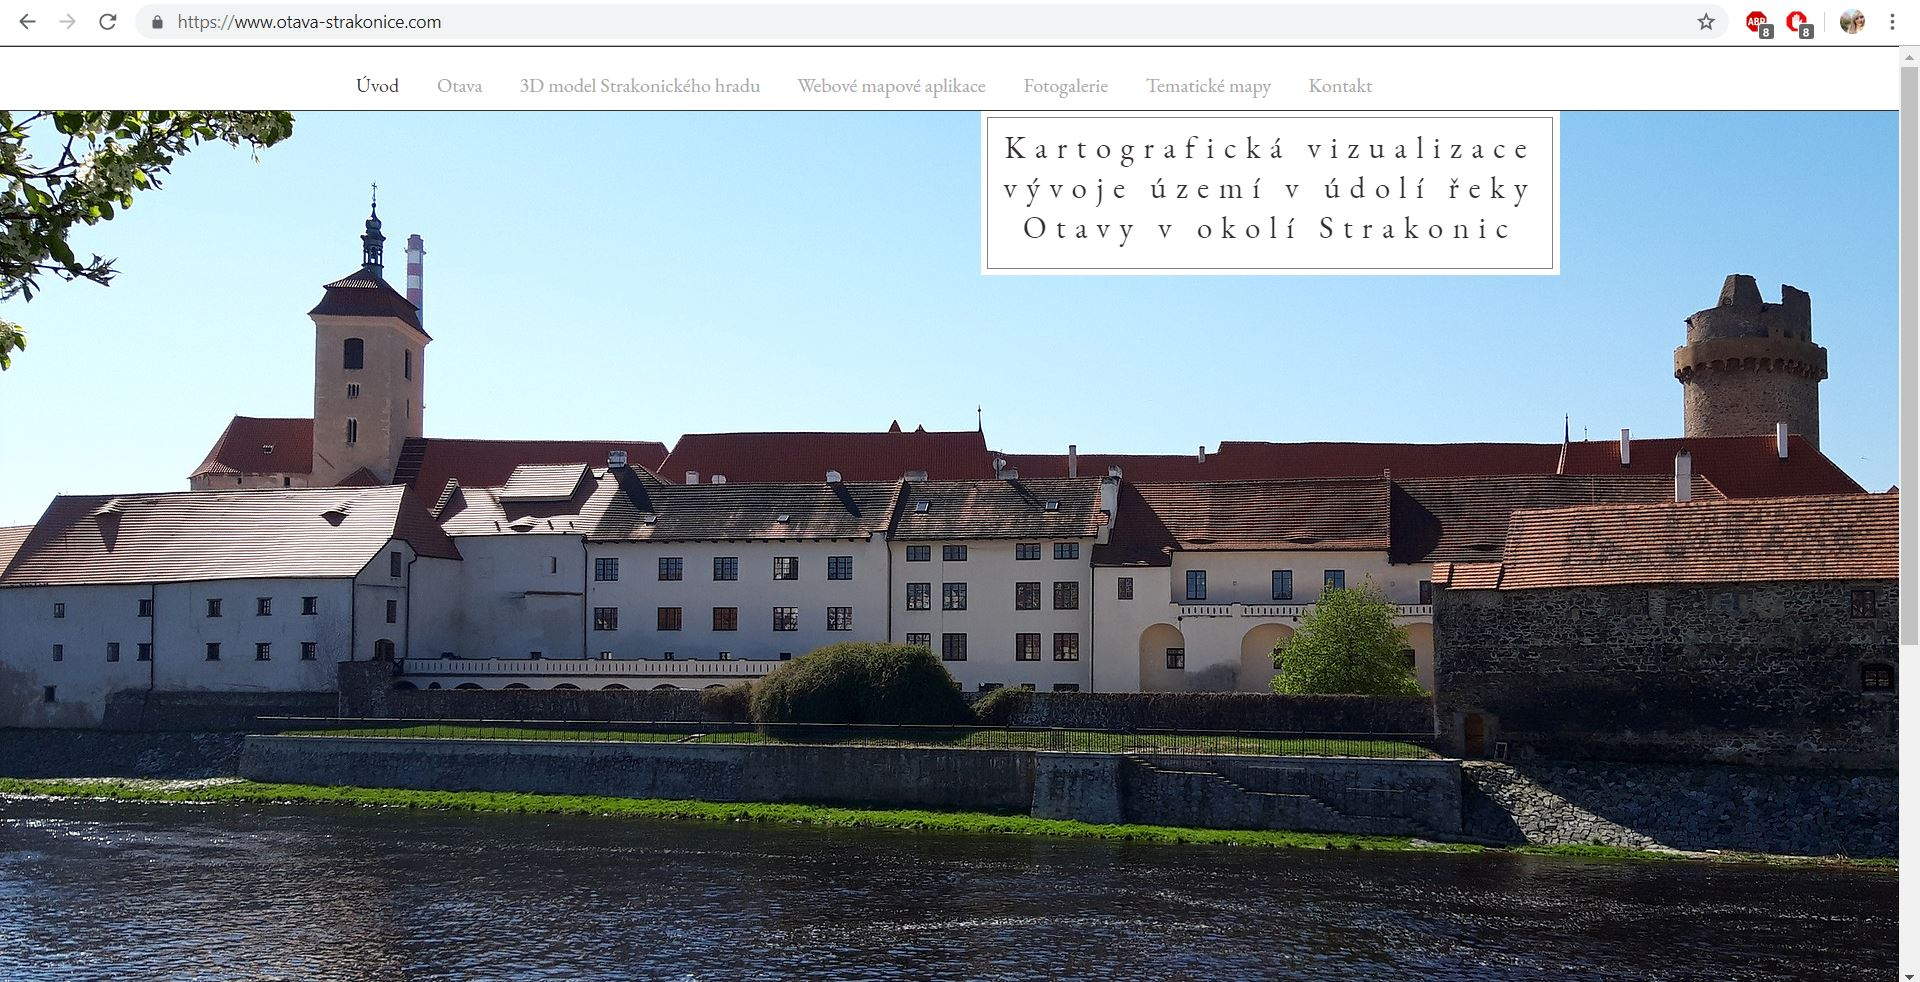
\includegraphics[width=14cm]{pics/web.jpg}
	\caption{Úvodní stránka}
	\label{obrazek:web}
\end{figure}


\section{Rozvržení webových stránek}


Webové stránky obsahují 6 hlavních stránek – Úvod, Otava, 3D model Strakonického hradu, Webové mapové aplikace, Fotogalerie, Tematické mapy a~Kontakt. Stránka Úvod obsahuje čtyři fotografie, které se s časovým intervalem prolínají a krátké představení stránky.



Na stránce Otava je vložena zvuková nahrávka z oblasti Podskalí podél řeky Otavy. Stránka obsahuje informace o řece a městech, kterými řeka protéká. Text na  stránce Otava byl převzat z této práce. Text je doplněn o fotografie řeky, které pořídila autorka. Poslední fotografie pochází ze soukromé sbírky Ladislava Hölla. 

Stránka 3D model Strakonického hradu obsahuje vložený objekt ze stránky 3D Warehouse. V rámci tohoto objektu je možné si model libovolně přiblížit či oddálit a prohlédnout z různých úhlů. Na stránce jsou také vložena dvě videa nahraná na server YouTube. Tato videa jsou vložena pro automatickou prohlídku vytvořeného modelu.

Na stránku webové mapové aplikace byly vloženy 2D a 3D webové mapové aplikace vytvořené na stránce ArcGIS Online. 

Stránka Fotogalerie obsahuje výběr fotografií řeky Otavy a významných objektů v jejím blízkém okolí. Zároveň stránka obsahuje podstránky, na nichž byla vytvořena srovnávací fotodokumentace. Z toho důvodu, že většina dochovaných historických fotografií zahrnuje Strakonický hrad, je vyobrazen na většině fotografií. Zároveň byly vloženy i srovnávací fotografie z povodní roku~2002, které oblast středního Pootaví silně zasáhly. Zveřejněné aktuální fotografie byly vytvářeny v období od ledna do května roku 2019. Na podstránce Otava ve Strakonicích jsou dvě poslední fotografie zapůjčeny od pana Ladislava Hölla, neboť jsou pořízeny z věží kostelů, kam nebyl zajištěn přístup.

\begin{figure}[h]
	\centering
	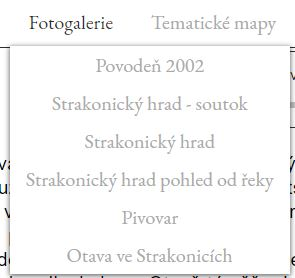
\includegraphics[width=5cm]{pics/foto.jpg}
	\caption{Podstránky stránky Fotogalerie}
	\label{obrazek:foto}
\end{figure}

Na stránce Tematické mapy je vytvořena galerie s volným výběrem vyobrazených map. Při rozkliknutí je u každé mapy popis s názvem města a~druhu kartografických podkladů. Vložené mapy jsou vytvářeny v zadaných měřítkách pro formát mapy A3. 

Stránka Kontakt obsahuje kontaktní formulář v případě dotazů a tlačítko pro sdílení na sociálních sítích. 


\section{Fotodokumentace}
Významnou částí webové stránky a celé práce je vytvořená srovnávací fotodokumentace. Za účelem pořízení fotografií pro zmíněnou fotodokumentaci a~textur modelu bylo nutné hrad několikrát navštívit. Navštívení hradu bylo nutné i z toho důvodu, že v současné době probíhá rozsáhlá rekonstrukce a~některé části hradu byly z toho důvodu zakryty lešením. 

\begin{figure}[h!]
	\centering
	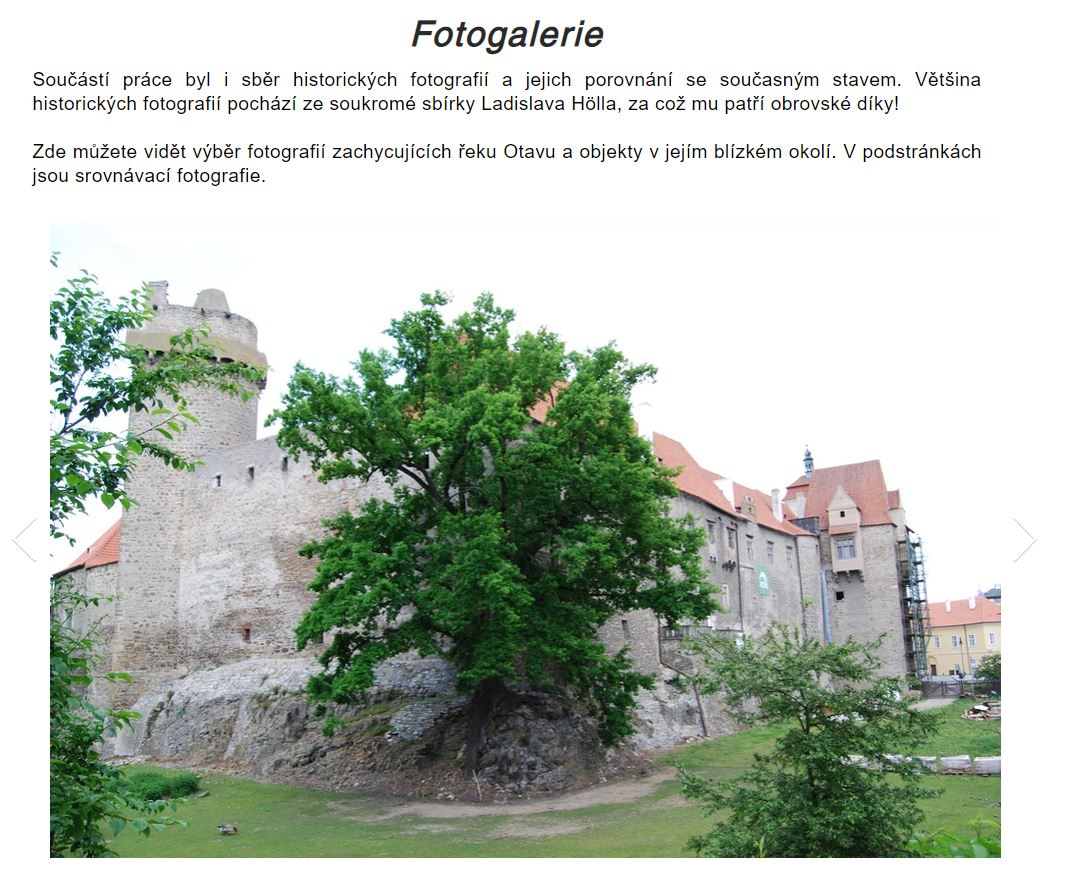
\includegraphics[width=14cm]{pics/fotogalerie.jpg}
	\caption{Stránka Fotogalerie}
	\label{obrazek:fotoga}
\end{figure}

V podstránkách Fotogalerie jsou následně srovnávací fotografie. Podstránky jsou rozděleny dle tématu, který je na fotografii vyobrazen. Na stránkách jsou následně vlevo umístěny historické fotografie a vpravo aktuální.


\begin{figure}[h!]
	\centering
	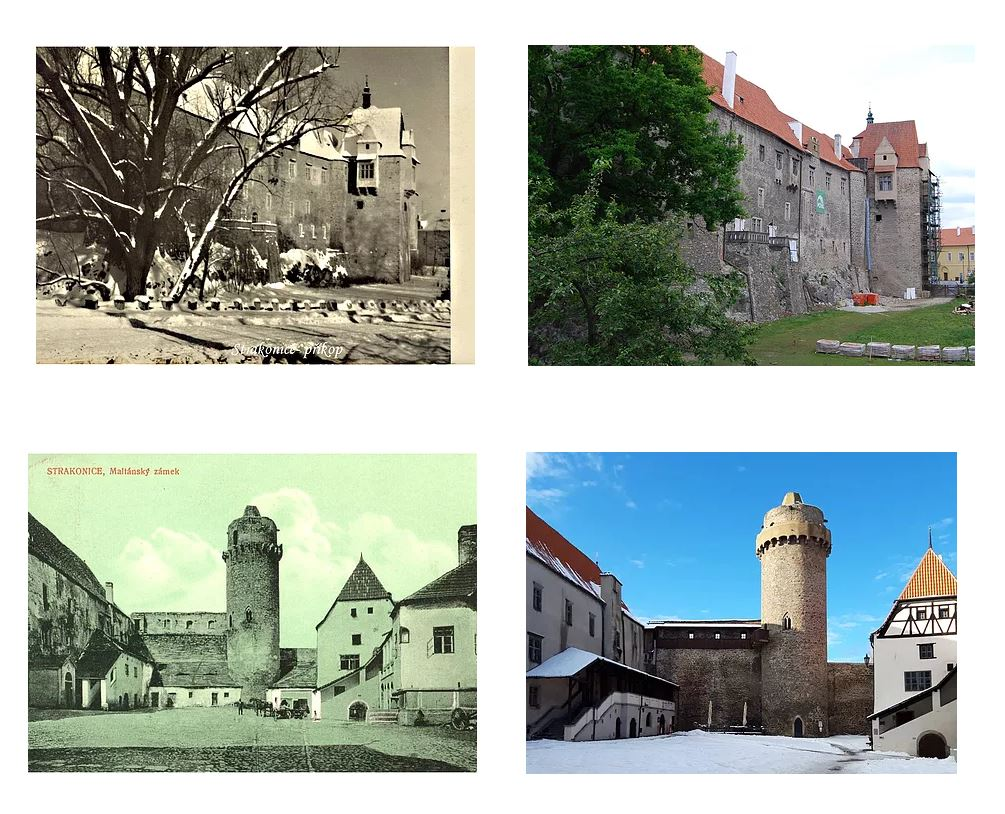
\includegraphics[width=16cm]{pics/srovnani.jpg}
	\caption{Ukázka srovnávacích fotografií zachycujících Strakonický hrad}
	\label{obrazek:srov}
\end{figure}

V rámci této práce jsou pro ukázku vybrána jen některá srovnání. Více fotografií lze nalézt na webových stránkách. Na obrázku č. \ref{obrazek:srov} lze vidět hradní příkop a věž Rumpál. Na obrázku č. \ref{obrazek:fotodok} je kostel sv. Markéty nacházející se poblíž soutoku Otavy s Volyňkou a Strakonický hrad pohledem od bývalé loděnice.

\clearpage

\begin{figure}[t!]
	\centering
	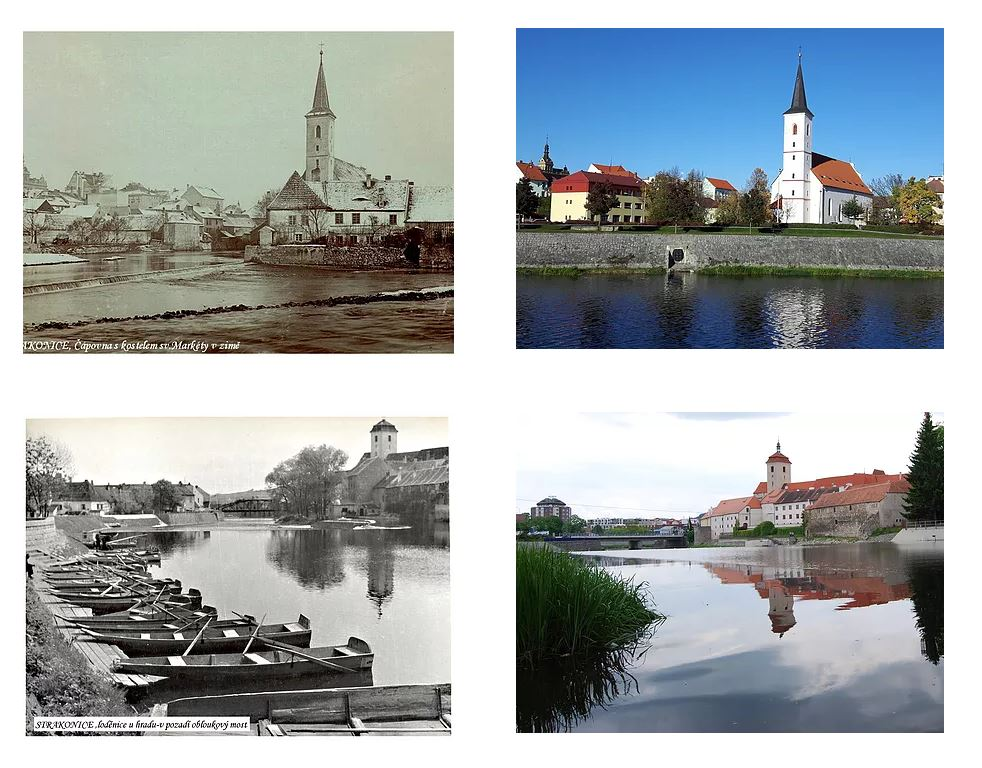
\includegraphics[width=16cm]{pics/fotodok1.jpg}
	\caption{Ukázka srovnávacích fotografií zachycujících řeku Otavu}
	\label{obrazek:fotodok}
\end{figure}

Pro webovou stránku byla vytvořena vlastní doména \textit{https://www.otava-strakonice.com/}. Na webových stránkách se stále pracuje a předpokládá se, že fotogalerie a srovnávací fotodokumentace se budou nadále rozšiřovat.

\chapter{Diskuze}
V současné době je velký zájem o historii a její porovnání s aktuálním stavem. Tato skutečnost lze vidět i na vyhotovených pracích. Za zmínku jistě stojí diplomová práce od Adély Dykastové  \cite{dykastova}, která zpracovávala historické mapové podklady a modelovala objekty pro město Kadaň. V této práci byla zvolena rozsáhlejší oblast, a to oblast středního Pootaví, tedy od Horažďovic po Strakonice. Tato oblast má, stejně jako město Kadaň, bohatou historii. Zpracování podkladových dat probíhalo obdobným způsobem, rastry byly georeferencovány na podkladech katastrálních map, aby při následné vizualizaci ve webových mapových aplikacích nebyly výrazné rozdíly. Vzhledem k malé oblasti mohla Adéla Dykastová vektorizovat objekty více typů a porovnávat jejich vývoj v rámci různých časových období. V případě rozšíření této práce by tato možnost byla zajisté vítána. Mohl by být porovnán vývoj krajiny, jak se změnil podíl orné půdy, lesů a luk na úkor zástavby. Při takto vytvořených prvcích by bylo následně také možné vypočítat koeficient ekologické stability, jenž udává poměr stabilních a nestabilních ekosystémů. Pomocí tohoto koeficientu lze zhodnotit, zda je území hojně využívané a přírodní struktury jsou narušené, či se jedná o přírodní krajinu s nízkou intenzitou využití člověkem. 

V práci byla zadaná oblast modelována z dat SMO–5, stejný způsob tvorby využila i Adina Slívová ve své diplomové práci \cite{adina}, v níž se zaměřila na oblast historického údolí Slap. Ve své práci narazila na několik problémů týkajících se špatně přiřazené nadmořské výšky vrstevnice či chybějícímu přesnému umístění výškové kóty. Rastry použité pro tuto práci naštěstí žádný obdobný problém neobsahovaly, přesto byla při vektorizaci zvýšená obezřetnost. V rámci této práce byly vyzkoušeny všechny způsoby tvorby vrstevnic, aby byl vybrán ten nejefektivnější, neboť bylo nutné zvektorizovat vrstevnice pro velké území. Nejvhodnější způsob byla poloautomatická tvorba vrstevnic. Při automatické tvorbě byly zvektorizovány i objekty, které s vrstevnicemi nemají nic společného, a tyto objekty bylo nutné následně důkladně prozkoumat a odstranit. 

Součástí výstupů této práce jsou i mapy měst, kterými Otava protéká.  O~výstupy této práce projevila zájem Šmidingerova knihovna ve Strakonicích, se kterou se momentálně jedná o možnosti vystavení map v prostorách vstupní haly knihovny na Strakonickém hradě. 

Součástí práce byla tvorba generalizovaného 3D modelu Strakonického hradu. Jedná se o rozsáhlý, členitý a velmi složitý komplex. Na hradě se snoubí téměř všechny architektonické styly od románského po barokní. V této práci je model využit pro dokreslení rázu krajiny, z~toho důvodu byl hrad generalizován. Dalším z důvodů výrazné generalizace byla paměťová náročnost programu CityEngine. Tento program má při nahrávání komplikovaných staveb problémy se zobrazením textur. Tento problém se nevyhnul ani Strakonickému hradu, u nějž se přes několik oprav nepodařilo vykreslit texturu hradní věže Rumpál. Navíc bylo pro publikování nutné odstranit textury z jižní strany hradu, které po importu do softwaru CityEngine byly náhodně rozmístěny po~celém objektu.



Vytvoření konkrétního objektu dodá oblasti na autentičnosti a vizuálně blíže přiblíží dané prostředí. Dle mapových podkladů se v oblasti nachází více významných budov, ať už se jedná o~kostely či například o~zámek Střelu. Součástí práce by do budoucna mohlo být rozšíření o vytvořené 3D modely těchto významných staveb. 

Při publikování dat ze softwaru CityEngine docházelo k problému s umístěním objektů. Přestože objekty v programu CityEngine měly totožné půdorysy s podkladovou  mapou, po publikování jsou objekty zhruba o 10 m posunuté. Na vině bude zřejmě vnitřní transformace, neboť surová data jsou v systému S-JTSK Krovak East North a ArcGIS Online data zobrazuje v systému Web Mercator. Tento problém byl konzultován s vedoucím práce, ale bohužel se jej nepodařilo odstranit. 

Neopomenutelnou součástí práce byl také sběr historických fotografií a~jejich porovnání s aktuálním stavem. Velké množství fotografií znázorňuje Strakonice, za uvážení by jistě stálo důkladnější prozkoumání archivů zbylých měst a rozšíření fotodokumentace o tyto fotografie. Zároveň by jistě bylo vhodné rozšířit fotogalerii o fotografie pořízené dronem. Tímto způsobem by bylo možné zmapovat větší část řeky.

Řeka byla ústředním tématem této práce. Za tímto účelem byly detailně prozkoumány a prostudovány materiály týkající se hydrologie, přestože v práci byly zmíněny jen okrajově. Hydrologie je velmi zajímavá věda a je úzce spjata s ekologií, která je v dnešní době často diskutovaná. Obzvláště v oblasti středního Pootaví se poblíž hydrologických objektů vyskytuje chráněná fauna a~flóra, některé z oblastí jsou součástí soustavy NATURA 2000. Ta spravuje evropsky významné lokality. Mezi tyto lokality patří například Kozlovská stráň, kde byl zaznamenán výskyt hořečku mnohotvarého, pastvina u Přešťovic spadající pod obec Slaník s bohatou květenou a obec Štěkeň, v níž se vyskytuje tesařík obrovský. Nesmím opomenout zmínit Tůně u Hajské, ve kterých se nacházejí bývalé sejpy po rýžování zlata a v okolí roste vzácný druh žebratky bahenní. Byl zaznamenán i velký zájem veřejnosti o ekologii. V dubnu roku 2019 uspořádal Český svaz ochránců přírody pomoc obojživelníkům při jejich jarní migraci. Dle záznamů bylo zachráněno 967 jedinců, většina byly ropuchy obecné, ale v menší míře se vyskytl i čolek obecný, skokan hnědý či blatnice skvrnitá.

Celkově je oblast velmi bohatá na přírodní památky. V prostředí Strakonicka se nachází mnoho památných stromů, několik přírodních studánek a přírodně krajinářsky významných lokalit. Při rozšíření práce by jistě stálo za úvahu detailnější prozkoumání těchto objektů a jejich prezentace formou webových aplikací.

Přestože tvorbu práce doprovázely různé komplikace, podařilo se splnit cíl práce a prezentovat výstupy prostřednictvím webové stránky. Webová stránka je na pohled čistá a přehledná. Jako velké plus vidím možnost porovnání dobových fotografií s aktuálním stavem, navíc mnoho z použitých fotografií není veřejně dostupných. Webová stránka je k dispozici na adrese \textit{https://www.otava-strakonice.com/}. Stránka zároveň obsahuje interaktivní výstupy, které jsou součástí této práce.

Velký důraz při práci byl kladen na samostatnost. Veškeré historické podklady od stavebních plánů hradu po sběr historických fotografií byl získán autorkou. Zároveň bylo pro potřebu fotodokumentace nutné získat aktuální snímky, které si autorka taktéž sama obstarala. Získání aktuálních fotografií výrazně ztěžovaly restaurátorské práce, při nichž byly po určitou dobu části hradu zakryty lešením. 

Součástí práce bylo i porovnání vytvořeného 3D modelu krajiny s již existujícím. V rámci této části byla blíže prozkoumána funkce \textit{Topo to raster}, která nabízí celou řadu vstupů a výpočetních parametrů. Při bližším zkoumání terénu a detailnějším zpracování by se dala práce rozšířit o příkré svahy, čímž by se docílilo kvalitnějších výsledků. Do vstupu mohly být vkládány i liniové prvky znázorňující tok řeky či polygony obsahující výjimky, kde by byla data ignorována. Vzhledem k tomu, že vytvořený rastr rozdílů výšek může být nicneříkající, byl z programu ArcMap uložen i histogram, který lépe zobrazuje výškové rozdíly.


Práce se sama o sobě zabývá velmi širokým tématem a zahrnuje velké území. Práci lze považovat za kvalitní zdroj při zpracování v prostředí ArcMap, neboť softwaru ArcMap je věnována velká část díla. Detailněji jsou popsány transformace, které se používají v ArcMapu při georeferencování. Velkým přínosem je také snaha o propojení několika různých softwarů a objektů z nich vypublikovaných.





\begin{conclusion}
Hlavním cílem práce byla vizualizace území v údolí řeky Otavy v okolí Strakonic, doplnění o vytvořený objekt Strakonického hradu a sběr historických fotografií. Všechny výstupy byly následně prezentovány na vytvořených webových stránkách.

Stěžejní část práce spočívala v georeferencování císařských povinných otisků map stabilního katastru. Vzhledem k velikosti oblasti bylo nutné zgeoreferencovat celkem 59 rastrů. Je zde nutné podotknout, že se jedná o počet rastrů, nikoliv katastrálních území. Zgeoreferencované rastry byly následně ořezány a ukládány do vytvořené geodatabáze. Georeferencování bylo náročné, neboť bylo nutné kontrolovat nejen střední chybu, ale také návaznost jednotlivých listů, zejména návaznost vodního toku. Po zpracování císařských povinných otisků stabilního katastru byly stejným způsobem zgeoreferencovány rastry SMO–5. 

Z podkladů císařských povinných otisků byly zvektorizovány vodní toky, budovy a lesy. Tato vrstva následně posloužila pro generování objektů v softwaru CityEngine, kde byla aplikována pravidla procedurálního modelování. Z~rastrů SMO–5 byly zvektorizovány vrstevnice a výškové kóty, které byly dále využity pro modelování krajiny. Vytvořená krajina byla porovnána s existujícím modelem krajiny DMR 5G. 

Pro autentičnost byl vytvořen 3D model Strakonického hradu v programu SketchUp, který doplnil vytvořené modely krajiny. Model byl vytvářen generalizovaný a velké množství dílčích částí bylo vkládáno ve formě textur. 

Výsledky ze softwaru CityEngine, ArcMap a ArcGIS Pro byly publikovány na server ArcGIS Online, kde byly pro interaktivní prohlížení vytvořeny webové mapové aplikace. Zároveň byla pro prezentování výsledků vytvořena webová stránka obsahující nejen výstupy, ale také stručnou historii měst a~vytvořenou srovnávací fotodokumentaci.





\end{conclusion}

\bibliographystyle{csn690}
\bibliography{mybibliographyfile}

\appendix

\chapter{Seznam použitých zkratek}
% seřadit podle abecedy
% \printglossaries
\begin{description}
	\item[Bpv] Balt po vyrovnání
	\item[CE] CityEngine
	\item[CPO] Císařské povinné otisky map stabilního katastru
	\item[ČMeS] Česká meteorologická společnost
	\item[ČÚZK] Český ústav zeměměřický a katastrální
	\item[DIBAVOD] Digitální báze vodohospodářských dat
	\item[DMR 5G] Digitální model reliéfu 5. generace
	\item[EPSG] European Petroleum Survey Group – databáze obsahující kódy zemských elipsoidů, geodetických dat, zeměpisných a kartografických souřadnicových systémů, měrných jednotek apod., každý souřadnicový systém má unikátní kód
	\item[ESRI] Environmental Systems Research Institute - jeden z největších světových producentů software GIS
	\item[GIS] Geografický informační systém
	\item[HTML] Hypertext Markup Language
	\item[JPG] Joint Photographic Experts Group
	\item[KMZ] Keyhole Markup Language
	\item[MNČ] Metoda nejmenších čtverců
	\item[SHP] Stavebně historický průzkum
	\item[SMO–5] Státní mapa 1 : 5 000 – odvozená
	\item[SÚRPMO] Státní ústav pro rekonstrukce památkových měst a objektů
	\item[S-JTSK] Systém jednotné trigonometrické sítě katastrální
	\item[TIFF] Tagged Image File Format
	\item[WMS] Web Map Service

\end{description}



\chapter{Obsah přiloženého CD}

\begin{figure}
	\dirtree{%
		.1 readme.txt\DTcomment{stručný popis obsahu CD}.
		.1 odkazy.txt\DTcomment{Odkazy na webové stránky výstupů}.
		.1 3D\_model\DTcomment{složka obsahující 3D model a video}.
		.1 LaTex\DTcomment{zdrojová forma práce ve formátu \LaTeX{}}.	
		.1 mapy\DTcomment{složka obsahující vytvořené mapy}.
		.1 text\DTcomment{text práce}.
		.2 DP\_Pasovska\_Petra\_2019\DTcomment{text práce v PDF}.	
	}
\end{figure}


\chapter{Tematické mapy}

\begin{enumerate}
\item [C.1] Skvělý
\item [C.1] Skvělý
\item [C.1] Skvělý
\end{enumerate}

\end{document}